\PassOptionsToPackage{hyphens}{url}
\documentclass[superscriptaddress, nofootinbib,  amsmath, amssymb, twocolumn]{revtex4-2} % twocolumn causing issues with neverending spillover into invisible area past first page

% \usepackage{balance}

% \usepackage[margin=1.5cm]{geometry} 
\usepackage[english]{babel}
\usepackage[utf8]{inputenc}
\usepackage[]{graphicx}
\usepackage{xspace}
\usepackage{siunitx}
\usepackage{mhchem}
\DeclareSIUnit\angstrom{\text {Å}}
\usepackage{orcidlink}
\usepackage{hyperref}
\usepackage{fontawesome5}
\usepackage{natmove}
\usepackage{placeins}

\usepackage{ifthen}        % For conditional statements


\usepackage{longtable}



% % Initialize a macro to keep track of seen project names
% \newcommand{\projectnamesseen}{}

% % Define a macro to select the appropriate social media icon
% \newcommand{\socialmediaicon}[1]{%
%     \IfSubStr{#1}{twitter.com}{\faTwitter}{%
%     \IfSubStr{#1}{linkedin.com}{\faLinkedin}{%
%     \IfSubStr{#1}{facebook.com}{\faFacebook}{%
%     \IfSubStr{#1}{instagram.com}{\faInstagram}{\faLink}}}}%
% }
% \DTLloadrawdb[keys={ProjectNum,ProjectLink,ProjectName,TeamName,FirstName,LastName,Email,Organization,Industry/Academia/Gov't,City,Address,GithubRepo,SocialMediaLink,VideoLink}]{stores}{test.csv}

\usepackage{xparse}
\usepackage[a-1b]{pdfx}
% \usepackage[allfiguresdraft]{draftfigure}

\usepackage[disable]{todonotes}
% \usepackage{todonotes}

\newcommand{\githublink}[2]{
  \href{https://github.com/#1/#2}{\faGithub\ \url{#1/#2}}
}

\newcommand{\twitterlink}[1]{
  \href{#1}{\faTwitter}
}

\newcommand{\zenodolink}[1]{
  \href{https://doi.org/#1}{\faArchive\ \url{#1}}
}

%https://twitter.com/SamCox822/status/1641484192566460416?s=20

\newcommand{\formatlinks}[3]{%
    \href{\ifx\empty#1\empty N/A\else#1\fi}{\faGithub}\,%
    \href{\ifx\empty#2\empty N/A\else#2\fi}{\faVideo}\,%
    \href{\ifx\empty#3\empty N/A\else#3\fi}{\faTwitter}  % Adjust the icon based on social media type
}


\newcommand{\hflogo}{%

\includegraphics[height=.9em]{figures/huggingface.png}
}

\newcommand{\huggingfacelink}[2]{
  \href{https://huggingface.co/spaces/#1/#2}{\hflogo \url{#1/#2}}
}

\newcommand{\huggingfacehublink}[2]{
  \href{https://huggingface.co/#1/#2}{\hflogo \url{#1/#2}}
}

% Adjusted Hyperref Setup for Automatically Colored Text Links
\hypersetup{
  colorlinks=true,       % Enables colored links
  breaklinks=true,
  urlcolor=blue,         % Sets the color of URL links
  linkcolor=blue,        % Sets the color of internal links
  citecolor=blue,        % Sets the color of citation links
  filecolor=blue,        % Sets the color of file links
  allcolors=blue,        % Ensures all link types are blue by default
  pdftitle={Title},      % PDF Title
  pdfauthor={Author}     % PDF Author
}

\usepackage[nameinlink,capitalise]{cleveref} %needs to appear after hyperref, https://tex.stackexchange.com/questions/396728/my-equations-referencing-not-working
\Crefname{figure}{Figure}{Figures} %needs to appear after hyperref and cleveref
\crefname{appsec}{Appendix}{Appendices}
\newcommand\crefrangeconjunction{--} % modify the reference style


% =====================================================
% packages for creating code listings 
\usepackage{listings, xcolor}
\definecolor{codegreen}{rgb}{0,0.6,0}
\definecolor{codegray}{rgb}{0.5,0.5,0.5}
\definecolor{codepurple}{rgb}{0.58,0,0.82}
\definecolor{tqblue}{HTML}{08293d}
\definecolor{backcolour}{HTML}{fefdf5}

\lstdefinestyle{pythonstyle}{
    backgroundcolor=\color{backcolour},   
    commentstyle=\color{codegreen},
    keywordstyle=\color{magenta},
    numberstyle=\tiny\color{codegray},
    stringstyle=\color{codepurple},
    basicstyle=\ttfamily\footnotesize\color{tqblue},
    breakatwhitespace=false,         
    breaklines=true,
    postbreak=\mbox{\textcolor{magenta}{$\hookrightarrow$}\space},                 
    captionpos=b,                    
    keepspaces=true,                 
    numbers=left,                    
    numbersep=5pt,                  
    showspaces=false,                
    showstringspaces=false,
    showtabs=false,                  
    tabsize=2
}

\lstset{style=pythonstyle}
\hbadness=99999 

\newcolumntype{C}{>{$}c<{$}}

\AtBeginDocument{%
  \heavyrulewidth=.08em
  \lightrulewidth=.05em
  \cmidrulewidth=.03em
  \belowrulesep=.65ex
  \belowbottomsep=0pt
  \aboverulesep=.4ex
  \abovetopsep=0pt
  \cmidrulesep=\doublerulesep
  \cmidrulekern=.5em
  \defaultaddspace=.5em
}



\usepackage[most]{tcolorbox}

\tcbset {
  base/.style={
    arc=0mm, 
    bottomtitle=0.5mm,
    boxrule=0mm,
    colbacktitle=black!10!white, 
    coltitle=black, 
    fonttitle=\bfseries, 
    left=2.5mm,
    leftrule=1mm,
    right=8.5mm,
    title={#1},
    toptitle=0.75mm, 
    width=\textwidth,
    breakable
  }
}

\definecolor{brandblue}{rgb}{0, 0.27843137254902, 0.466666666666667}
\newtcolorbox{agentinteraction}[1]{
  colframe=brandblue, 
  base={#1}
}


\definecolor{brandbred}{rgb}{0.63921568627451, 0, 0}
\newtcolorbox{agentinteraction2}[1]{
  colframe=brandbred, 
  base={#1}
}


\newtcolorbox{subbox}[1]{
  colframe=black!30!white,
  base={#1}
  }

\usepackage [autostyle, english = american]{csquotes}
\MakeOuterQuote{"}
\usepackage[acronym, nonumberlist]{glossaries}
\glsdisablehyper
\makeglossaries

\newacronym{llm}{LLM}{large language model}
\newacronym{gpt}{GPT}{generative pretrained transformer}
\newacronym{api}{API}{application programming interface}
\newacronym{ml}{ML}{machine learning}
\newacronym{lift}{LIFT}{language-interfaced fine-tuning}
\newacronym{icl}{ICL}{in-context learning}
\newacronym{peft}{PEFT}{parameter efficient fine-tuning}
\newacronym{lora}{LoRA}{low-rank adaptors}
\newacronym{gpr}{GPR}{Gaussian process regression}
\newacronym{ga}{GA}{genetic algorithm}
\newacronym{svm}{SVM}{support vector machine}
\newacronym{rf}{RF}{random forest}

\newacronym{ord}{ORD}{Open Reaction Database}
\newacronym{bo}{BO}{Bayesian optimization}
\newacronym{id}{ID}{inverse design}
\newacronym{mad}{MAD}{median absolute deviation}
\newacronym{eln}{ELN}{electronic lab notebook}
\newacronym[shortplural=LIMS]{lims}{LIMS}{laboratory information system}
\newacronym{ui}{UI}{user interface}
\newacronym{nlm}{NLM}{national library of medicine} 
\newacronym{dft}{DFT}{density functional theory}
\newacronym{cot}{COT}{chain of thought}
\newacronym{gui}{GUI}{graphical user interface}
\newacronym{pdb}{PDB}{protein data bank}
\newacronym{rlhf}{RLHF}{reinforcement learning from human feedback}
\newacronym{json}{JSON}{JavaScript object notation}
\newacronym{smiles}{SMILES}{simplified molecular-input line-entry system}
\newacronym{selfies}{SELFIES}{self-referencing embedded strings}
\newacronym{ai}{AI}{artificial intelligence}
\newacronym{nlp}{NLP}{natural language processing}
\newacronym{ner}{NER}{named entity recognition}
\newacronym{cas}{CAS}{Chemical Abstract Services}
\newacronym{mae}{MAE}{mean absolute error}
\newacronym{inchi}{InChI}{international chemical identifier}
\newacronym{mapi}{MAPI}{Materials Project \gls{api}}
\newacronym{rouge}{ROUGE}{Recall-Oriented Understudy for Gisting Evaluation}
\newacronym{html}{HTML}{HyperText Markup Language}
\newacronym{doi}{DOI}{digital object identifier}
\newacronym{ocr}{OCR}{optical character recognition}

\usepackage{tabularx} % For flexible tables with adjustable column widths
\usepackage{booktabs} % For better table lines (\toprule, \midrule, \bottomrule)
\usepackage{cleveref}

\let\originalcite\cite
\renewcommand{\cite}[1]{\unskip~\originalcite{#1}}

\usepackage{setspace}

% \clubpenalty=10000
% \widowpenalty=10000
% \displaywidowpenalty=10000
\usepackage{titlesec}

\titlespacing{\subsection}
    {0pt}{9pt}{6pt}

\usepackage{array}
\usepackage{ragged2e}
\usepackage{nicefrac}
\usepackage[caption=false]{subfig}

\newcolumntype{P}[1]{>{\raggedright\arraybackslash}p{#1}}

\begin{document}

\title{Bayesian Optimization Hackathon for Chemistry and Materials}

% %ToDo: add contributed equally indication for participants

\newcommand{\equalcont}{\thanks{These authors contributed equally}}

\author{Kevin~Maik~Jablonka~\orcidlink{0000-0003-4894-4660}}
\email{mail@kjablonka.com}
\affiliation{Laboratory of Molecular Simulation (LSMO), Institut des Sciences et Ing\'{e}nierie Chimiques, Ecole Polytechnique F\'{e}d\'{e}rale de Lausanne (EPFL), Sion, Valais, Switzerland.}

\author{Qianxiang Ai~\orcidlink{0000-0002-5487-2539}}
\equalcont
\affiliation{Department of Chemical Engineering, Massachusetts Institute of Technology, Cambridge, Massachusetts 02139, United States.}

%\email{qai@mit.edu}


\author{Alexander~Al-Feghali~\orcidlink{0009-0004-8377-7049}} 
\equalcont
%\email{alexander.al-feghali@mail.mcgill.ca}
\affiliation{Department of Chemistry, McGill University, Montreal, Quebec, Canada.}

\author{Shruti~Badhwar~\orcidlink{0000-0002-3167-5348}}
\equalcont
\affiliation{Reincarnate Inc.}  
%\email{shruti@reincarnateartificial.com}

\author{Joshua~D.~Bocarsly~\orcidlink{0000-0002-7523-152X}}
\equalcont
 \affiliation{Yusuf Hamied Department of Chemistry, University of Cambridge, Lensfield Road, Cambridge, CB2 1EW, United Kingdom.} 
 
%\email{jb2382@cam.ac.uk} 

\author{Andres~M~Bran~\orcidlink{0000-0002-4432-3667}}
\equalcont
\affiliation{Laboratory of Artificial Chemical Intelligence (LIAC), Institut des Sciences et Ing\'{e}nierie Chimiques, Ecole Polytechnique F\'{e}d\'{e}rale de Lausanne (EPFL), Lausanne, Switzerland.} 
\affiliation{National Centre of Competence in Research (NCCR) Catalysis, Ecole Polytechnique F\'{e}d\'{e}rale de Lausanne (EPFL), Lausanne, Switzerland.}


\author{Stefan~Bringuier~\orcidlink{0000-0001-6753-1437}}
\equalcont
\affiliation{Independent Researcher, San Diego, CA, United States.}
%\email{stefanbringuier@gmail.com}

\author{L.~Catherine~Brinson~\orcidlink{0000-0003-2551-1563}}
\equalcont
\affiliation{Mechanical Engineering and Materials Science, Duke University, United States.}
%\email{cate.brinson@duke.edu}



\author{Defne~Circi~\orcidlink{0000-0002-5761-0198}}
\equalcont
\affiliation{Mechanical Engineering and Materials Science, Duke University, United States.}
%\email{defne.circi@duke.edu}

\author{Sam~Cox~\orcidlink{0000-0002-4441-9327}}
\equalcont
\affiliation{Department of Chemical Engineering, University of Rochester, United States.}
%\email{swrig30@ur.rochester.edu}

\author{Wibe~A.~de~Jong~\orcidlink{0000-0002-7114-8315}} 
\equalcont
\affiliation{Applied Mathematics and Computational Research Division, Lawrence Berkeley National Laboratory, Berkeley, CA 94720, United States.
}

\author{Matthew~L.~Evans~\orcidlink{0000-0002-1182-9098}}
\equalcont
 \affiliation{Institut de la Matière Condensée et des Nanosciences (IMCN), UCLouvain, Chemin des Étoiles 8, Louvain-la-Neuve, 1348, Belgium.}
 \affiliation{Matgenix SRL, 185 Rue Armand Bury, 6534 Gozée, Belgium.}
 %\email{matthew.evans@uclouvain.be}

 \author{Nicolas~Gastellu~\orcidlink{0000-0002-4052-076X}}
 \equalcont
\affiliation{Department of Chemistry, McGill University, Montreal, Quebec, Canada.}
%\email{nicolas.gastellu@mail.mcgill.ca} 

\author{Jerome~Genzling~\orcidlink{0009-0007-4728-1478}} 
\equalcont
\affiliation{Department of Chemistry, McGill University, Montreal, Quebec, Canada.}
%\email{jerome.genzling@mail.mcgill.ca}

\author{Mar\'ia~Victoria~Gil~\orcidlink{0000-0002-2258-3011}}
\equalcont
\affiliation{Instituto de Ciencia y Tecnolog\'ia del Carbono (INCAR), CSIC, Francisco Pintado Fe 26, 33011 Oviedo, Spain.}
%\email{victoria.gil@incar.csic.es}

\author{Ankur~K.~Gupta~\orcidlink{0000-0002-3128-9535}}
\equalcont
\affiliation{Applied Mathematics and Computational Research Division, Lawrence Berkeley National Laboratory, Berkeley, CA 94720, United States.
}


\author{Alishba~Imran}
\equalcont
\affiliation{Computer Science, University of California, Berkeley, Berkeley CA 94704, United States.}

\author{Sabine~Kruschwitz~\orcidlink{0000-0002-6296-4417}}
\equalcont
\affiliation{Bundesanstalt für Materialforschung und -prüfung, Unter den Eichen 87, 12205 Berlin, Germany.}
%\email{Sabine.Kruschwitz@bam.de}

\author{Anne~Labarre~\orcidlink{0000-0003-4939-3928}}
\equalcont
\affiliation{Department of Chemistry, McGill University, Montreal, Quebec, Canada.}
 %\email{Anne.Labarre@mail.mcgill.ca}  

\author{Jakub~Lála~\orcidlink{0000-0002-5424-5260}}
\equalcont
\affiliation{Francis Crick Institute, 1 Midland Rd, London NW1 1AT, United Kingdom.}
%\email{jakublala@gmail.com}
 
\author{Tao~Liu~\orcidlink{0000-0002-1082-5570}}
\equalcont
\affiliation{Department of Chemistry, McGill University, Montreal, Quebec, Canada.}
 %\email{tao.liu7@mail.mcgill.ca} 

\author{Steven~Ma~\orcidlink{0000-0006-9448-7332}}
\equalcont
\affiliation{Department of Chemistry, McGill University, Montreal, Quebec, Canada.}
 %\email{Steven.Ma@mail.mcgill.ca} 

\author{Sauradeep~Majumdar~\orcidlink{0000-0002-2095-3082}}
\equalcont
\affiliation{Laboratory of Molecular Simulation (LSMO), Institut des Sciences et Ing\'{e}nierie Chimiques, Ecole Polytechnique F\'{e}d\'{e}rale de Lausanne (EPFL), Sion, Valais, Switzerland.}
%\email{sauradeep.majumdar@epfl.ch}

\author{Garrett~W.~Merz~\orcidlink{0000-0003-4737-3931}}
\equalcont
\affiliation{American Family Insurance Data Science Institute, University of Wisconsin-Madison, Madison WI 53706, United States.}


\author{Nicolas~Moitessier~\orcidlink{0000-0001-6933-2079}}
\equalcont
\affiliation{Department of Chemistry, McGill University, Montreal, Quebec, Canada.}
%;  Department of Chemistry, McGill University, Montreal, Quebec, Canada; orcid.org/; 
%\email{nicolas.moitessier@mcgill.ca}

\author{Elias~Moubarak~\orcidlink{0000-0001-8271-6800}}
\equalcont
\affiliation{Laboratory of Molecular Simulation (LSMO), Institut des Sciences et Ing\'{e}nierie Chimiques, Ecole Polytechnique F\'{e}d\'{e}rale de Lausanne (EPFL), Sion, Valais, Switzerland.}
%\email{elias.moubarak@epfl.ch}



\author{Beatriz~Mouriño~\orcidlink{0000-0003-1670-3985}}
\equalcont
\affiliation{Laboratory of Molecular Simulation (LSMO), Institut des Sciences et Ing\'{e}nierie Chimiques, Ecole Polytechnique F\'{e}d\'{e}rale de Lausanne (EPFL), Sion, Valais, Switzerland.}
%\email{beatriz.buenomourino@epfl.ch}

\author{Brenden~Pelkie~\orcidlink{0000-0001-7638-6366}}
\equalcont
\affiliation{Department of Chemical Engineering, University of Washington, Seattle, WA 98105, United States.} 
%\email{bgpelkie@uw.edu} 

\author{Michael~Pieler~\orcidlink{0000-0001-9186-7045}}
\equalcont
\affiliation{OpenBioML.org}
\affiliation{Stability.AI}
%\email{ michael.pieler@gmail.com}

\author{Mayk~Caldas~Ramos~\orcidlink{0000-0001-5336-2847}}
\equalcont
\affiliation{Department of Chemical Engineering, University of Rochester, United States.}
%\email{mcaldasr@ur.rochester.edu}

\author{Bojana~Ranković~\orcidlink{0000-0002-1476-6686}}
\equalcont
\affiliation{Laboratory of Artificial Chemical Intelligence (LIAC), Institut des Sciences et Ing\'{e}nierie Chimiques, Ecole Polytechnique F\'{e}d\'{e}rale de Lausanne (EPFL), Lausanne, Switzerland.}
\affiliation{National Centre of Competence in Research (NCCR) Catalysis, Ecole Polytechnique F\'{e}d\'{e}rale de Lausanne (EPFL), Lausanne, Switzerland.}


\author{Jacob~N.~Sanders~\orcidlink{0000-0002-2196-4234}}
\equalcont
\affiliation{Department of Chemistry and Biochemistry, University of California, Los Angeles, CA 90095, United States.}
%\email{jacosand@gmail.com}




\author{Philippe~Schwaller~\orcidlink{0000-0003-3046-6576}}
\equalcont
\affiliation{Laboratory of Artificial Chemical Intelligence (LIAC), Institut des Sciences et Ing\'{e}nierie Chimiques, Ecole Polytechnique F\'{e}d\'{e}rale de Lausanne (EPFL), Lausanne, Switzerland.}
\affiliation{National Centre of Competence in Research (NCCR) Catalysis, Ecole Polytechnique F\'{e}d\'{e}rale de Lausanne (EPFL), Lausanne, Switzerland.}

 
\author{Marcus~Schwarting}
\equalcont
 \affiliation{Department of Computer Science, University of Chicago, Chicago IL 60490, United States.}
 %\email{meschw04@uchicago.edu}


\author{Jiale~Shi~\orcidlink{0000-0002-5447-3925}}
\equalcont
\affiliation{Department of Chemical Engineering, Massachusetts Institute of Technology, Cambridge, Massachusetts 02139, United States.}
 %\email{jialele@mit.edu}
 
 \author{Berend~Smit~\orcidlink{0000-0003-4653-8562}}
%\email{berend.smit@epfl.ch}
\equalcont
\affiliation{Laboratory of Molecular Simulation (LSMO), Institut des Sciences et Ing\'{e}nierie Chimiques, Ecole Polytechnique F\'{e}d\'{e}rale de Lausanne (EPFL), Sion, Valais, Switzerland.}

\author{Ben~E.~Smith~\orcidlink{0000-0001-9673-2449}}
\equalcont
 \affiliation{Yusuf Hamied Department of Chemistry, University of Cambridge, Lensfield Road, Cambridge, CB2 1EW, United Kingdom.} 
%\email{bs542@cam.ac.uk} 


\author{Joren~Van~Herck~\orcidlink{009-0005-5108-5061}}
\equalcont
\affiliation{Laboratory of Molecular Simulation (LSMO), Institut des Sciences et Ing\'{e}nierie Chimiques, Ecole Polytechnique F\'{e}d\'{e}rale de Lausanne (EPFL), Sion, Valais, Switzerland.}
%\email{joren.vanherck@epfl.ch}


\author{Sean~Warren~\orcidlink{0000-0002-3670-0354}}
\equalcont
%\affiliation{}
%\email{sean.warren@gatech.edu}



\author{Sylvester~Zhang}
\equalcont
\affiliation{Department of Chemistry, McGill University, Montreal, Quebec, Canada.}

\author{Xiaoqi~Zhang\orcidlink{0000-0002-6507-6490}}
\equalcont
\affiliation{Laboratory of Molecular Simulation (LSMO), Institut des Sciences et Ing\'{e}nierie Chimiques, Ecole Polytechnique F\'{e}d\'{e}rale de Lausanne (EPFL), Sion, Valais, Switzerland.}
%\email{xiaoqi.zhang@epfl.ch}


\author{Ghezal~Ahmad~Zia~\orcidlink{0000-0002-9082-9423}} 
\equalcont
\affiliation{Bundesanstalt für Materialforschung und -prüfung, Unter den Eichen 87, 12205 Berlin, Germany.}
%\email{Ghezal-Ahmad.Zia@bam.de} 



% organiziers 

\author{KJ~Schmidt}
%\email{kj.schmidt913@gmail.com}
\affiliation{Globus, University of Chicago, Data Science and Learning Division, Argonne National Lab, United States.}

\author{Ian~Foster~\orcidlink{0000-0003-2129-5269}}
\affiliation{Department of Computer Science, University of Chicago, Data Science and Learning Division, Argonne National Lab, United States.}

\author{Ben~Blaiszik~\orcidlink{0000-0002-5326-4902}}
\email{blaiszik@uchicago.edu}
\affiliation{Globus, University of Chicago, Data Science and Learning Division, Argonne National Lab, United States.}




\author{Sterling~G.~Baird}
\author{Mehrad~Ansari}
\affiliation{Acceleration Consortium, 700 University Ave.\ Suite 1001, Toronto, ON M5G 1X6}

% one footnote, shared by both authors
\email[Corresponding authors: ]{\{sterling.baird,\,mehrad.ansari\}@utoronto.ca}

\author{Zartashia ~Afzal}
% \email{chemistzartashiaafzal@gmail.com}
\affiliation{ICodeGuru, Canal Road, Quaid-i-Azam Campus, Lahore, Punjab, Pakistan.}

\author{Qianxiang~Ai}
% \email{qai@mit.edu}
\affiliation{Massachusetts Institute of Technology, Massachusetts Institute of Technology, 77 Massachusetts Ave, Cambridge, MA 02139, United States.}

\author{Alexander~Al-Feghali}
% \email{alexander.al-feghali@mail.mcgill.ca}
\affiliation{McGill University, Canada, 845 Rue Sherbrooke O, Montréal, QC H3A 0G4.}

\author{Mathieu~Alain}
% \email{mathieu.alain.21@ucl.ac.uk}
\affiliation{University College London, Gower Street, London WC1E 6BT.}

\author{Roozbeh~Alishahian}
% \email{rooz.alishahian@mail.utoronto.ca}
\affiliation{University of Toronto, 27 King's College Circle, Toronto, ON M5S 1A1, Canada.}

\author{Matias~Altamirano}
% \email{matias.altamirano.22@ucl.ac.uk}
\affiliation{University College London, Gower Street, London WC1E 6BT.}

\author{Thomas~Andrews}
% \email{tsandrews@student.unimelb.edu.au}
\affiliation{University of Melbourne, CSIRO, Parkville VIC 3052.}

\author{Andy Sode~Anker}
% \email{ansoan@dtu.dk}
\affiliation{Technical University of Copenhagen and Oxford University, Anker Engelunds Vej 411, 2800 Kongens Lyngby, Danmark \& Mansfield Rd, Oxford OX1 3TA, United Kingdom.}

\author{Rija~Ansari}
% \email{rija.ansari@nrc-cnrc.gc.ca}
\affiliation{National Research Council of Canada, 1200 Montreal Road, Ottawa ON, K1A 0R6.}

\author{Samuel Ampofo~Appiah}
\affiliation{Ghana National Gas Company, Ghana National Gas Company, Gas House, 7th Avenue, Ridge West, Accra, Ghana.}

\author{Raul~Astudillo}
% \email{rastudil@caltech.edu}
\affiliation{California Institute of Technology, 315 Annenberg IST Center, 330 S Chester Ave, Pasadena, CA 91125, United States.}

\author{Ruhana~Azam}
% \email{ruhana@stanford.edu}
\affiliation{Stanford University, 353 Jane Stanford Way, Stanford, CA, 94305.}

\author{Mohammed~Azzouzi}
% \email{mohammed.azzouzi15@imperial.ac.uk}
\affiliation{Imperial College London, Exhibition Rd, South Kensington, London SW7 2AZ.}

\author{Suneel Kumar~BVS}
% \email{Suneelkumar.bvs@gmail.com}
\affiliation{Atomicas AI solutions private limited}

\author{Ben~Blaiszik}
% \email{blaiszik@uchicago.edu}
\affiliation{University of Chicago, 9700 S. Cass Avenue, Lemont, IL, USA.}

\author{Anna~Borisova}
% \email{anna.borisova@epfl.ch}
\affiliation{EPFL, Station 06, CH-1015 Lausanne, Switzerland.}

\author{Andres~Bran}
% \email{andres.marulandabran@epfl.ch}
\affiliation{EPFL, NCCR Catalysis, Station 06, CH-1015 Lausanne, Switzerland.}

\author{Darby~Brown}
\affiliation{EMD Electronics, Frankfurter Str. 250, 64293 Darmstadt, Germany.}

\author{Pengfei~Cai}
% \email{pengfeic@mit.edu}
\affiliation{Massachusetts Institute of Technology, 77 Massachusetts Avenue Cambridge, MA 02139.}

\author{Ting-Yeh~Chen}
% \email{chen.11026@buckeyemail.osu.edu}
\affiliation{The Ohio State University, 281 W Lane Ave, Columbus, OH 43210.}

\author{Curtis~Chong}
% \email{curtischong5@gmail.com}
% \affiliation{nan, nan.}

\author{Samantha~Corapi}
% \email{s.corapi@mail.utoronto.ca}
\affiliation{University Of Toronto, 27 King's College Circle, Toronto, ON M5S 1A1, Canada.}

\author{Mark~Croxall}
\affiliation{University of Toronto, 27 King's College Cir, Toronto, ON M5S 1A1.}

\author{Gbetondji~Dovonon}
% \email{gbetondji@matterhorn.studio}
\affiliation{University College London, Gower Street, London WC1E 6BT.}

\author{Jose Manuel Napoles~Duarte}

\author{Andrew~Falkowski}
% \email{andrew.falkowski@utah.edu}
\affiliation{University of Utah, University of Utah, 201 Presidents Circle, Salt Lake City, UT 84112, United States.}

\author{Giuseppe~Fisicaro}
% \email{giuseppe.fisicaro@imm.cnr.it}
\affiliation{Institute for Microelectronics and Microsystems (IMM), National Research Council (CNR), Institute for Microelectronics and Microsystems (IMM), National Research Council (CNR), Via del Fosso del Cavaliere 100, 00133 Rome, Italy.}

\author{Martin~Fitzner}
% \email{martin.fitzner@merckgroup.com}
\affiliation{Merck KGaA, Darmstadt, Germany, Frankfurter Straße 250, 64293 Darmstadt, Germany.}

\author{Quinn~Gallagher}
% \email{qg1361@princeton.edu}
\affiliation{Princeton University, Department of Chemical and Biological Engineering, Princeton University, Princeton, New Jersey 08540.}

\author{Sabah~Gaznaghi}
% \email{s.gaznaghi@uq.edu.au}
\affiliation{University of Queensland, Building 75, Cooper Rd, St Lucia QLD 4067, Australia.}

\author{Jérôme~Genzling}
% \email{jerome.genzling@mail.mcgill.ca}
\affiliation{McGill University, 845 Rue Sherbrooke O, Montréal, QC H3A 0G4.}

\author{Christoph~Griehl}
% \email{griehl@mpi-magdeburg.mpg.de}
\affiliation{Max Planck Institute for Dynamics of Complex Technical Systems , Sandtorstraße 1, 39112 Magdeburg, Germany.}

\author{Ryan-Rhys~Griffiths}
% \email{ryangriff123@gmail.com}
\affiliation{FutureHouse, 1405 Minnesota St, San Francisco, CA 94107.}

\author{Taicheng~Guo}
% \email{tguo2@nd.edu}
\affiliation{University of Notre Dame, Holy Cross Dr, Notre Dame, IN 46556.}

\author{Kehan~Guo}
% \email{kguo2@nd.edu}
\affiliation{University of Notre Dame, Holy Cross Dr, Notre Dame, IN 46556.}

\author{Nipun~Gupta}
% \email{nipun.gupta@utoronto.ca}
\affiliation{Acceleration Consortium, 700 University Ave suite 1001, Toronto, ON M5G 1X6.}

\author{Ankur~Gupta}
% \email{ankur@lbl.gov}
\affiliation{Lawrence Berkeley National Laboratory, 1 Cyclotron Rd, Berkeley, CA 94720.}

\author{Mohammad~Haddadnia}

\affiliation{University Of Harvard, Harvard University, Massachusetts Hall, Cambridge, MA 02138, United States.}

\author{Yuyang~Han}
% \email{yuyanghan@g.ucla.edu}
\affiliation{University of California, Los Angeles, 607 Charles E Young Dr E, Los Angles, CA 90093.}

\author{Karim Ben~Hicham}
\affiliation{RWTH Aachen, Templergraben 55, 52062 Aachen, Germany.}

\author{Joscha~Hoche}
% \email{joscha.hoche@merckgroup.com}
\affiliation{Merck KGaA, Darmstadt, Germany, Frankfurter Straße 250, 64293 Darmstadt, Germany.}

\author{Alexander V.~Hopp}
% \email{alexander.hopp@merckgroup.com}
\affiliation{Merck KGaA, Darmstadt, Germany, Frankfurter Straße 250, 64293 Darmstadt, Germany.}

\author{Marko~Huang}
% \email{marko.huang@mail.utoronto.ca}
\affiliation{Department of Chemistry, University of Toronto, Lash Miller Chemical Laboratories, 80 St.George Street.}

\author{Ayodeji~Ijishakin}
% \email{ayoijish@outlook.com}
\affiliation{University College London, Gower Street, London WC1E 6BT.}

\author{Ramsey~Issa}
% \email{ramseyissa@gmail.com}
\affiliation{University of Utah, University of Utah, 201 Presidents Circle, Salt Lake City, UT 84112, United States.}

\author{Yeonghun~Kang}
% \email{dudgns1675@kaist.ac.kr}
\affiliation{KAIST, KAIST (Korea Advanced Institute of Science and Technology), 291 Daehak-ro, Yuseong-gu, Daejeon 34141, South Korea.}

\author{Jungtaek~Kim}
% \email{jungtaek.kim.mail@gmail.com}
\affiliation{University of Pittsburgh, 3700 O'Hara St, Pittsburgh, PA 15261, United States.}

\author{Akshay~Kudva}
% \email{kudva.7@buckeyemail.osu.edu}
\affiliation{The Ohio State University, 281 W Lane Ave, Columbus, OH 43210.}

\author{Rubén~Laplaza}
% \affiliation{nan, nan.}

\author{Magdalena~Lederbauer}
% \email{mlederbauer@ethz.ch}
\affiliation{ETH Zurich, EPFL, Station 06, CH-1015 Lausanne, Switzerland.}

\author{Shi Xuan~Leong}
% \email{shixuan.leong@utoronto.ca}
\affiliation{Department of Chemistry, University of Toronto, Lash Miller Chemical Laboratories, 80 St.George Street.}

\author{Paul W.~Leu}
% \email{pleu@pitt.edu}
\affiliation{University of Pittsburgh, 3700 O'Hara St, Pittsburgh, PA 15261, United States.}

\author{Viola Muning~Li}
% \email{viola.muning-li@external.merckgroup.com}
\affiliation{Merck KGaA, Darmstadt, Germany, Frankfurter Straße 250, 64293 Darmstadt, Germany.}

\author{Mingxuan~Li}
% \email{mil152@pitt.edu }
\affiliation{University of Pittsburgh, 3700 O'Hara St, Pittsburgh, PA 15261, United States.}

\author{Tao~Liu}
% \email{tao.liu7@mail.mcgill.ca}
\affiliation{McGill University, Canada, 845 Rue Sherbrooke O, Montréal, QC H3A 0G4.}

\author{Stanley~Lo}
% \email{stanley.lo@mail.utoronto.ca}
\affiliation{University of Toronto, 27 King's College Circle, Toronto, ON M5S 1A1, Canada.}

\author{Jakub~Lála}
% \email{jl24018@ic.ac.uk}
\affiliation{Imperial College London, Exhibition Rd, South Kensington, London SW7 2AZ, United Kingdom.}

\author{Osman~Mamun}
% \email{mamun.che06@gmail.com}
% \affiliation{nan, nan.}

\author{Joseph~Manning}
\affiliation{University of Manchester, Oxford Rd, Manchester M13 9PL, United Kingdom.}

\author{Owen~Melville}
% \email{owen.melville@utoronto.ca}
\affiliation{Acceleration Consortium, 700 University Ave suite 1001, Toronto, ON M5G 1X6.}

\author{Michail~Mitsakis}
% \email{mitsakismichail@gmail.com}
\affiliation{Technical University of Denmark (DTU), Argous 64 \& Potamou 77, Kifissia, Athens, Greece.}

\author{Cameron~Movassaghi}
% \email{csmova@g.ucla.edu}
\affiliation{University of California, Los Angeles, 607 Charles E Young Dr E, Los Angles, CA 90093.}

\author{Madhav Reddy~Muthyala}
% \email{muthyala.7@buckeyemail.osu.edu}
\affiliation{The Ohio State University, 281 W Lane Ave, Columbus, OH 43210.}

\author{Marcel~Müller}
% \email{marcel.mueller@thch.uni-bonn.de}
\affiliation{Merck KGaA, Darmstadt, Germany / University of Bonn, Frankfurter Straße 250, 64293 Darmstadt, Germany.}

\author{Bozhao~Nan}
% \email{bnan@nd.edu}
\affiliation{University of Notre Dame, Holy Cross Dr, Notre Dame, IN 46556.}

\author{Vijay~Narasimhan}
\affiliation{EMD Electronics, Frankfurter Str. 250, 64293 Darmstadt, Germany.}

\author{Duc~Nguyen}
% \email{nqduc@stanford.edu}
\affiliation{Stanford University, 353 Jane Stanford Way, Stanford, CA, 94305.}

\author{Daniele~Ongari}
% \email{daniele.ongari@syensqo.com}
\affiliation{Syensqo , Viale Lombardia 20, Bollate, Italy.}

\author{Anthony~Onwuli}
% \email{anthony.onwuli16@imperial.ac.uk}
\affiliation{Imperial College London, Imperial College London, Exhibition Road, South Kensington, London SW7 2BX, United Kingdom.}

\author{Can~Özkan}
% \email{c.ozkan@tudelft.nl}
\affiliation{TU Delft, Mekelweg 5, 2628CD Delft, the Netherlands.}

\author{Sergio~Pablo-Garcia}
% \email{sp.garcia@utoronto.ca}
\affiliation{University of Toronto, Department of Chemistry, University of Toronto, Lash Miller Chemical Laboratories, 80 St.George Street.}

\author{Elton~Pan}
% \email{eltonpan@mit.edu}
\affiliation{Massachusetts Institute of Technology, 77 Massachusetts Avenue Cambridge, MA 02139.}

\author{Ratish~Panda}
% \email{ratishp2001@gmail.com}
\affiliation{Birla Institute of Technology, Mesra, Jharkhand 835215, India.}

\author{Sean~Park}
% \email{seanhs.park@mail.utoronto.ca}
\affiliation{University Of Toronto, University of Toronto, 27 King's College Circle, Toronto, ON M5S 1A1, Canada.}

\author{Jaehee~Park}
% \email{jaeheepark@uchicago.edu}
\affiliation{University of Chicago, 5801 S Ellis Ave, Chicago, IL 60637.}

\author{Brenden~Pelkie}
% \email{bgpelkie@uw.edu}
\affiliation{University of Washington, 3819 Okanogan Lane NE, Seattle, WA, 98195, USA.}

\author{Dieter~Plessers}
% \email{dieter.plessers@kuleuven.be}
\affiliation{KU Leuven, Celestijnenlaan 200F, 3001 Leuven, Belgium.}

\author{Tobias~Plötz}
% \email{tobias.ploetz@merckgroup.com}
\affiliation{Merck KGaA, Darmstadt, Germany, Frankfurter Straße 250, 64293 Darmstadt, Germany.}

\author{Utkarsh~Pratiush}
% \email{upratius@vols.utk.edu}
\affiliation{University of Tennessee, Knoxville, TN 37996, United States.}

\author{Ella M.~Rajaonson}
% \email{ella.rajaonson@mail.utoronto.ca}
\affiliation{University Of Toronto, University of Toronto, 27 King's College Circle, Toronto, ON M5S 1A1, Canada.}

\author{Bojana~Ranković}
% \email{bojana.rankovic@epfl.ch}
\affiliation{EPFL, NCCR Catalysis, Station 06, CH-1015 Lausanne, Switzerland.}

\author{Jarett~Ren}
% \email{jren25@jhu.edu}
\affiliation{Johns Hopkins University, 3400 N. Charles Street, Baltimore, MD 21218.}

\author{Rim~Rihana}
% \email{rim.rihana@merckgroup.com}
\affiliation{Merck KGaA, Darmstadt, Germany, Frankfurter Straße 250, 64293 Darmstadt, Germany.}

\author{Jurgis~Ruza}
% \email{jruza@mit.edu}
\affiliation{Massachusetts Institute of Technology, 77 Massachusetts Avenue Cambridge, MA 02139.}

\author{Akhil~S. Nair}
% \email{nair@fhi-berlin.mpg.de}
\affiliation{Fritz-Haber Institute of the Max-Planck Society,  Faradayweg 4-6, D-14195 Berlin, Germany.}

\author{Carter~Salbego}
% \email{carter.w.salbego@gmail.com}
\affiliation{University of Utah, University of Utah, 201 Presidents Circle, Salt Lake City, UT 84112, United States.}

\author{Erick Lopez~Saldivar}

\affiliation{Autonomous University of Chihuahua, Autonomous University of Chihuahua, Av. Escorza 900, Colonia Centro, 31000 Chihuahua, Chih., Mexico.}

\author{Arifin~San}
% \email{fin_ari@jsr.co.jp}
\affiliation{JSR Corporation, JSR Bioscience and informatics R\&D center (JSR BiRD), 3-103-9 Tonomachi, Kawasaki-ku, Kawasaki, Kanagawa 210-0821, Japan.}

\author{Christina~Schenk}
% \email{christina.schenk@imdea.org}
\affiliation{IMDEA Materials Institute, Calle Eric Kandel 2, Tecnogetafe,  28906 Getafe (Madrid), Spain.}

\author{Stefan P.~Schmid}
% \email{schmiste@ethz.ch}
\affiliation{ETH Zurich, Vladimir-Prelog-Weg 1, 8093 Zurich, Switzerland.}

\author{Dylan~Schubert}

\affiliation{Matterhorn Studio, Walton Street, Oxford, UK.}

\author{Philippe~Schwaller}
% \email{philippe.schwaller@epfl.ch}
\affiliation{EPFL, NCCR Catalysis, Station 06, CH-1015 Lausanne, Switzerland.}

\author{Cher-Tian~Ser}
% \email{serchertian@gmail.com}
\affiliation{University of Toronto, Department of Chemistry, University of Toronto, Lash Miller Chemical Laboratories, 80 St.George Street.}

\author{Maitreyee~Sharma Priyadarshini}
% \email{msharmap@vt.edu}
\affiliation{Virginia Tech, Virginia Tech, 925 Prices Fork Road, Blacksburg, VA 24061, United States.}

\author{Yuxin~Shen}
% \email{y.shen-80@sms.ed.ac.uk}
\affiliation{University of Edinburgh, CH Waddington Building, King's Buildings, Max Born Crescent, Edinburgh, EH9 3BF, United Kingdom.}

\author{Kevin~Shen}

\affiliation{NobleAI, 345 California St Suite 600, San Francisco, CA 94104, United States.}

\author{Jiale~Shi}
% \email{jialeshi@mit.edu}
\affiliation{Massachusetts Institute of Technology, 77 Massachusetts Ave, Cambridge, MA 02139, United States.}

\author{Farshud~Sorourifar}
% \email{sorourifar.1@buckeyemail.osu.edu}
\affiliation{The Ohio State University, 281 W Lane Ave, Columbus, OH 43210.}

\author{Adrian~Šošić}
% \email{adrian.sosic@merckgroup.com}
\affiliation{Merck Life Science KGaA, Darmstadt, Germany, Frankfurter Straße 250, 64293 Darmstadt, Germany.}

\author{Taylor~Sparks}
% \email{sparks@eng.utah.edu}
\affiliation{University of Utah, University of Utah, 201 Presidents Circle, Salt Lake City, UT 84112, United States.}

\author{Jan Christopher~Spies}
% \email{j_spie17@uni-muenster.de}
\affiliation{University of Muenster, Corrensstraße 40, 48149 Münster, Germany.}

\author{Felix~Strieth-Kalthoff}
% \email{strieth-kalthoff@uni-wuppertal.de}
\affiliation{University of Wuppertal, Germany, Gaußstraße 20, 42119 Wuppertal, Germany.}

\author{Suraj~Sudhakar}
% \email{surajsi@uchicago.edu}
\affiliation{University of Chicago, 5801 S Ellis Ave, Chicago, IL 60637.}

\author{Aditya~Sundar}

\author{Alessio~Tamburro}
% \email{alessio.tamburro@syensqo.com}
\affiliation{Syensqo, 350 George Patterson blvd, Bristol, US.}

\author{Clara~Tamura}
% \email{clarant2@uw.edu}
\affiliation{University of Washington, 3900 E Stevens Way NE, Seattle, WA 98195, United States.}

\author{Yifeng (Oliver)~Tang}
% \email{yifengt@uchicago.edu}
\affiliation{University of Chicago, 5801 S Ellis Ave, Chicago, IL 60637.}

\author{Dandan~Tang}
% \email{gux8df@virginia.edu}
\affiliation{University of Virginia, University of Virginia, 1827 University Ave, Charlottesville, VA 22903, United States.}

\author{Nikhil~Thota}
% \email{nthota2@jhu.edu}
\affiliation{Johns Hopkins University, 3400 N. Charles Street, Baltimore, MD 21218.}

\author{Mohammad Erfan~Toloue Sadegh Azadi}
% \email{mohammad.tolouesadeghazadi@mail.mcgill.ca}
\affiliation{McGill University, Canada, 845 Rue Sherbrooke O, Montréal, QC H3A 0G4.}

\author{Gary~Tom}
% \email{gtom@cs.utoronto.ca}
\affiliation{University Of Toronto, University of Toronto, 27 King's College Circle, Toronto, ON M5S 1A1, Canada.}

\author{Sang~Truong}
% \email{sttruong@cs.stanford.edu}
\affiliation{Stanford University, 353 Jane Stanford Way, Stanford, CA, 94305.}

\author{Ricardo~Valencia Albornoz}
% \email{r.g.valencia-albornoz@sms.ed.ac.uk}
\affiliation{University of Edinburgh, CH Waddington Building, King's Buildings, Max Born Crescent, Edinburgh, EH9 3BF, United Kingdom.}

\author{Luis~Walter}
% \email{walter@thphys.uni-heidelberg.de}
\affiliation{Heidelberg University, Philosophenweg 19, 69120 Heidelberg.}

\author{Lawrence~Wang}
\affiliation{Erthos, 2735 Matheson Blvd E 5, Mississauga, ON L4W 4M8.}

\author{Fanjin~Wang}
% \email{fanjin.wang.20@ucl.ac.uk}
\affiliation{University College London, Department of Mechanical Engineering, University College London, London, WC1E 7JE, United Kingdom.}

\author{Andrew~Wang}
% \email{ac.wang@mail.utoronto.ca}
\affiliation{Department of Chemistry, University of Toronto, Lash Miller Chemical Laboratories, 80 St.George Street.}

\author{Yiran ~Wang}
% \email{ywang580@mit.edu}
\affiliation{Massachusetts Institute of Technology, 77 Massachusetts Ave, Cambridge, MA 02139, United States.}

\author{Jeff~Watchorn}
% \email{jeff.watchorn@utoronto.ca}
\affiliation{Acceleration Consortium, 700 University Ave suite 1001, Toronto, ON M5G 1X6.}

\author{Benjamin~Weiser}
% \email{benjamin.weiser@mail.mcgill.ca}
\affiliation{McGill University, 845 Rue Sherbrooke O, Montréal, QC H3A 0G4.}

\author{Geemi~Wellawatte}
% \email{gwellawatte@gmail.com}
\affiliation{EPFL, Station 06, CH-1015 Lausanne, Switzerland.}

\author{Alexander~Wieczorek}
% \email{Alexander.Wieczorek@empa.ch}
\affiliation{Empa – Swiss Federal Laboratories for Materials Science and Technology, Ueberlandstrasse 129, Dübendorf, CH-8600 Switzerland.}

\author{Tim~Würger}
% \email{tim.wuerger@hereon.de}
\affiliation{Helmholtz-Zentrum Hereon, Max-Planck-Str. 1, 21502 Geesthacht, Germany.}

\author{Ilya~Yakavets}
% \email{i.yakavets@utoronto.ca}
\affiliation{Acceleration Consortium, 700 University Ave suite 1001, Toronto, ON M5G 1X6.}

\author{Jakob~Zeitler}
% \email{jakob@matterhorn.studio}
\affiliation{Matterhorn Studio, Walton Street, Oxford, UK.}

% % Counter too large

\author{Sylvester~Zhang}
% \email{sylvester.zhang@mail.mcgill.ca}
\affiliation{McGill University, 845 Rue Sherbrooke O, Montréal, QC H3A 0G4.}

\author{Yimu~Zhao}
% \email{yimu.zhao@utoronto.ca}
\affiliation{Acceleration Consortium, 700 University Ave suite 1001, Toronto, ON M5G 1X6.}

\author{Yanqiao~Zhu}
% \email{yzhu@cs.ucla.edu}
\affiliation{University of California, Los Angeles, 607 Charles E Young Dr E, Los Angles, CA 90093.}

\author{Ruijie (Ray)~Zhu}
% \email{rzhu16@uchicago.edu}
\affiliation{University of Chicago, 5801 S Ellis Ave, Chicago, IL 60637.}

\author{Yunheng~Zou}
% \email{y94zou@uwaterloo.ca}
\affiliation{University of Waterloo, 200 University Avenue West, Waterloo, Ontario, N2L 3G1.}




\begin{abstract}
The Acceleration Consortium and Merck KGaA hosted a 2-day virtual hackathon on March 27-28, 2024, bringing together scientists to explore, collaborate, and innovate in the field of Bayesian optimization for the physical sciences. Participants were encouraged to select or develop Bayesian optimization algorithms, apply them to benchmarking tasks, design new benchmarks, create instructional tutorials, and describe real-world applications. With over 100 participants across 60 academic, industry, and government organizations located in 38 cities, 14 countries, and 4 continents, this was a global event. % https://chatgpt.com/share/f6cd733f-1126-4151-86c5-d4b59d158dc3
The outputs from this event, including developed algorithms, benchmarks, and tutorials, will serve as valuable resources for the research community, in addition to the new skills learned and connections formed. Released projects and general information are available at \url{https://ac-bo-hackathon.github.io/} and other locations linked from individual project pages. This event demonstrates the potential of community-driven research efforts to accelerate advances in Bayesian optimization in chemistry and materials science.
\end{abstract}

\maketitle



% ToDo: 
% emphasize tooling/constrained prompting/guidance 

\todo[inline]{automate authors.tex based on the google sheet (maybe some info needed from credit form}

\section{Introduction}

\Gls{bo} has emerged as a powerful tool in optimizing complex and expensive-to-evaluate functions, often outperforming traditional search methods in a variety of scientific domains such as optimizing composition and processing parameters to maximize alloy yield strength or identifying synthesis pathways that maximize efficacy of HIV drugs (\cref{fig:intro-bo}). Hackathons help people to connect, gain skills, and flesh out new ideas. In the words of Michelle Duke, the "Hackathon Queen":

\begin{quote}
A hackathon is a short competition where people work together in teams to solve problems and challenges by coming up with solutions and ideas.
\end{quote}

\begin{figure}
    \centering
    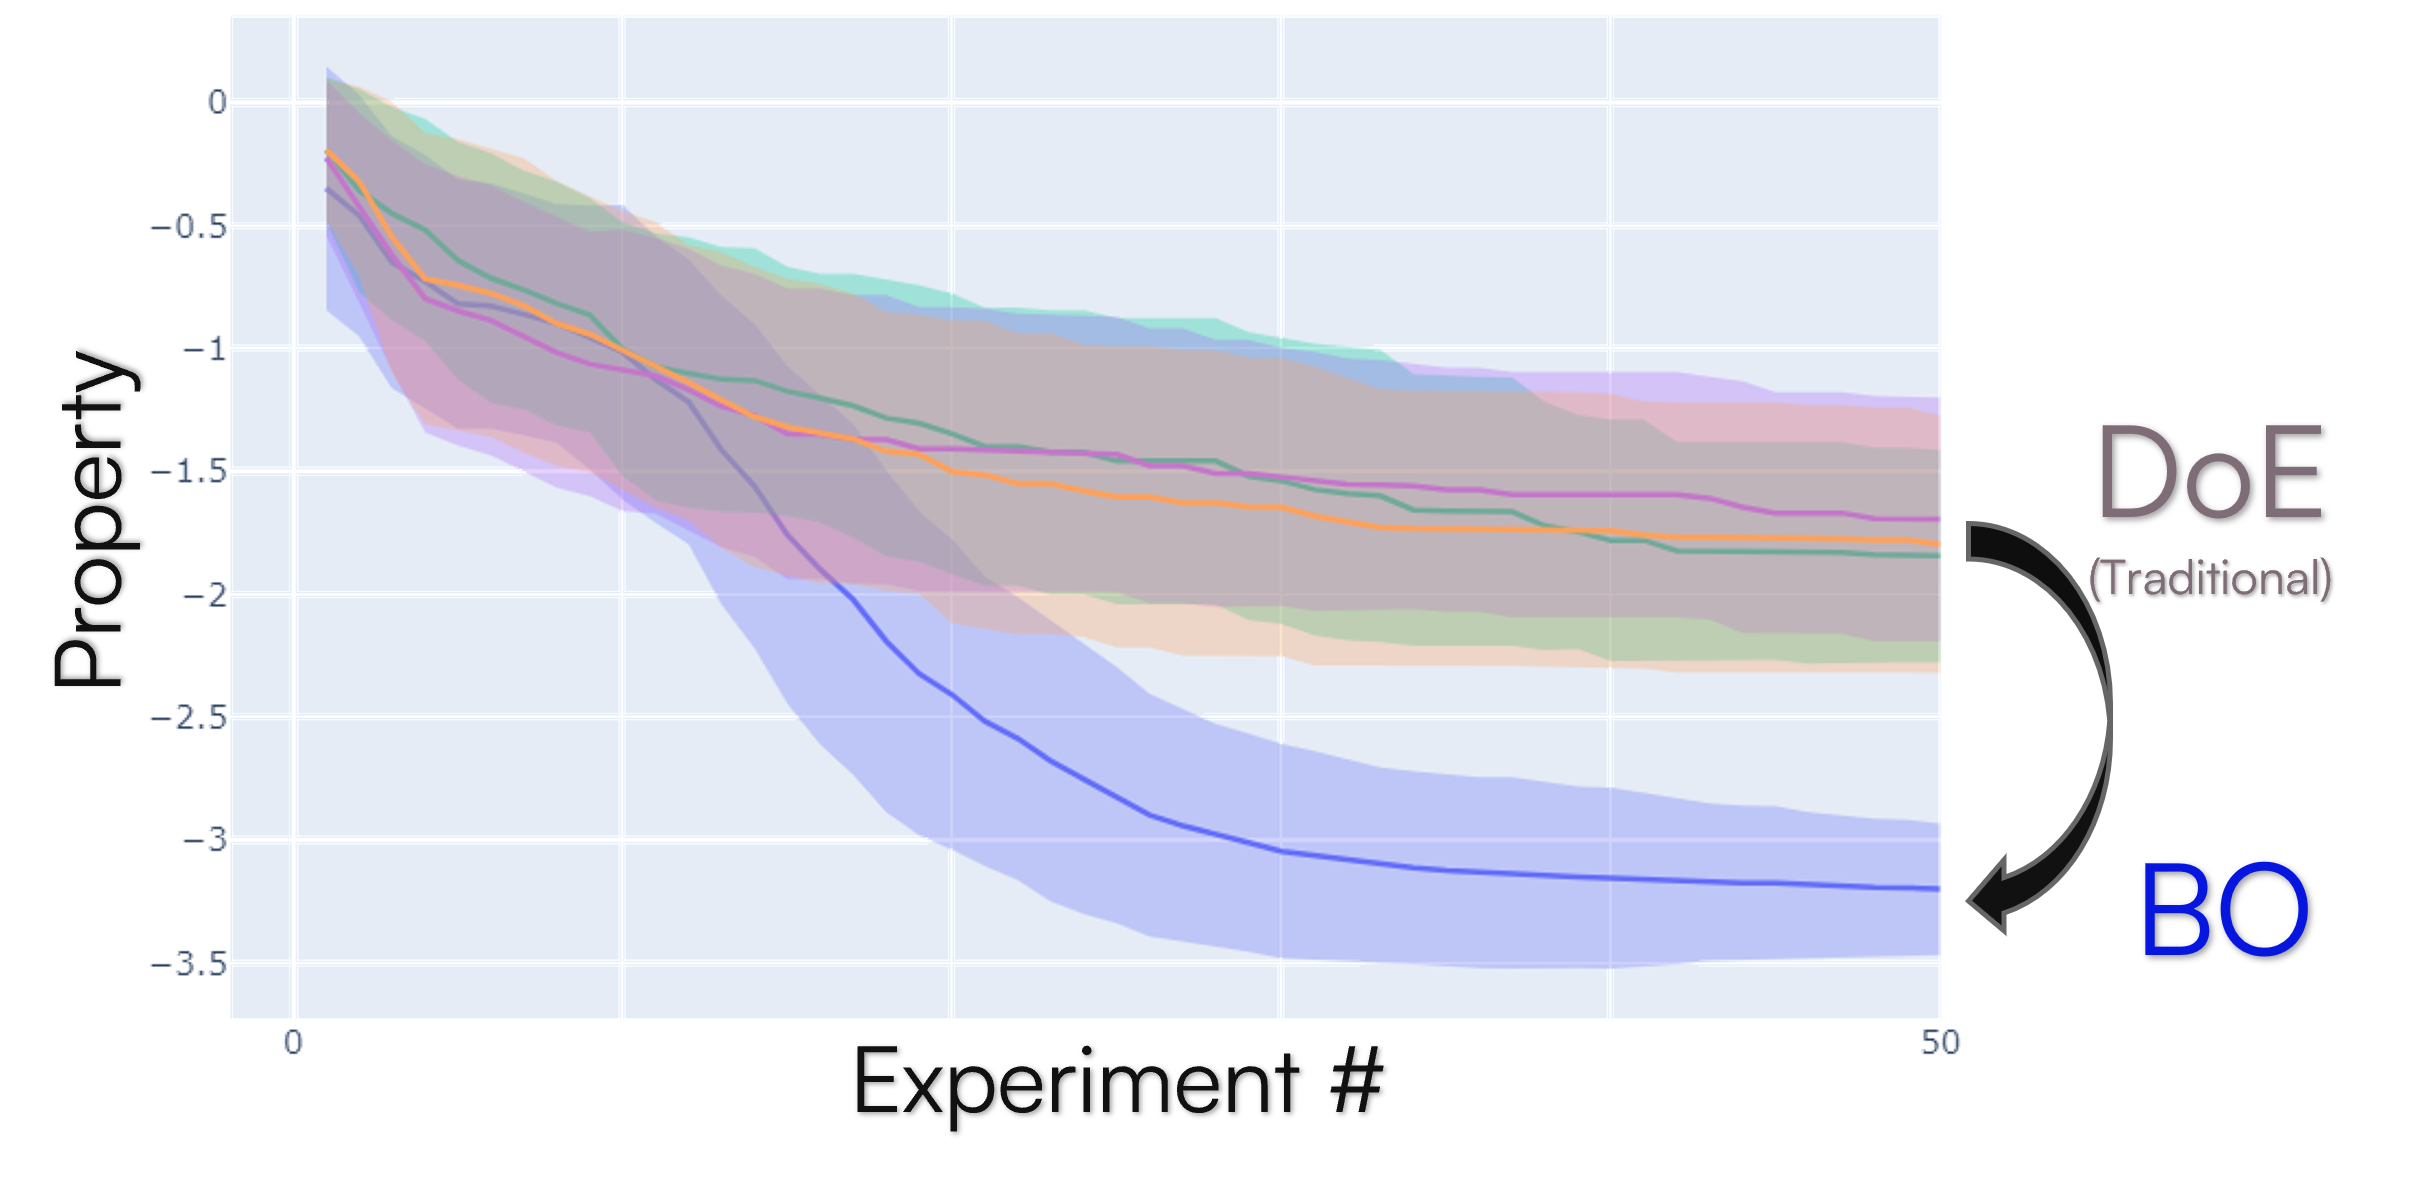
\includegraphics[width=1\linewidth]{latex/figures/intro-bo.png}
    \caption{Optimization traces for traditional design of experiment (DoE) methods compared with \gls{bo}, typically outperforms. \Gls{bo} uses a smart model to predict where to look next in an experiment to find the best results with few experiments \cite{baird_building_2023}.}
    \label{fig:intro-bo}
\end{figure}

The goal of the AC BO Hackathon was to leverage the expertise of a diverse, global community to advance the development and application of \gls{bo} techniques for solving critical challenges in the physical sciences. The hackathon also aimed to foster collaboration and knowledge sharing among participants from different backgrounds, including academia, national laboratories, government agencies, and private industry. The event attracted 120 active participants from 44 teams, representing 41 academic institutions, 12 national labs, and 9 companies. Likewise, the participants were located in 38 cities, 14 countries, and 4 continents (\cref{fig:map}). A full list of projects, including links to the corresponding GitHub repositories, submission video, and social media post are provided in \cref{tab:projects}.

% \onecolumngrid % (https://tex.stackexchange.com/a/214834/224861)
% % don't remove this linebreak 


\begin{figure*}
    \centering
    % \captionsetup{justification=centering}
    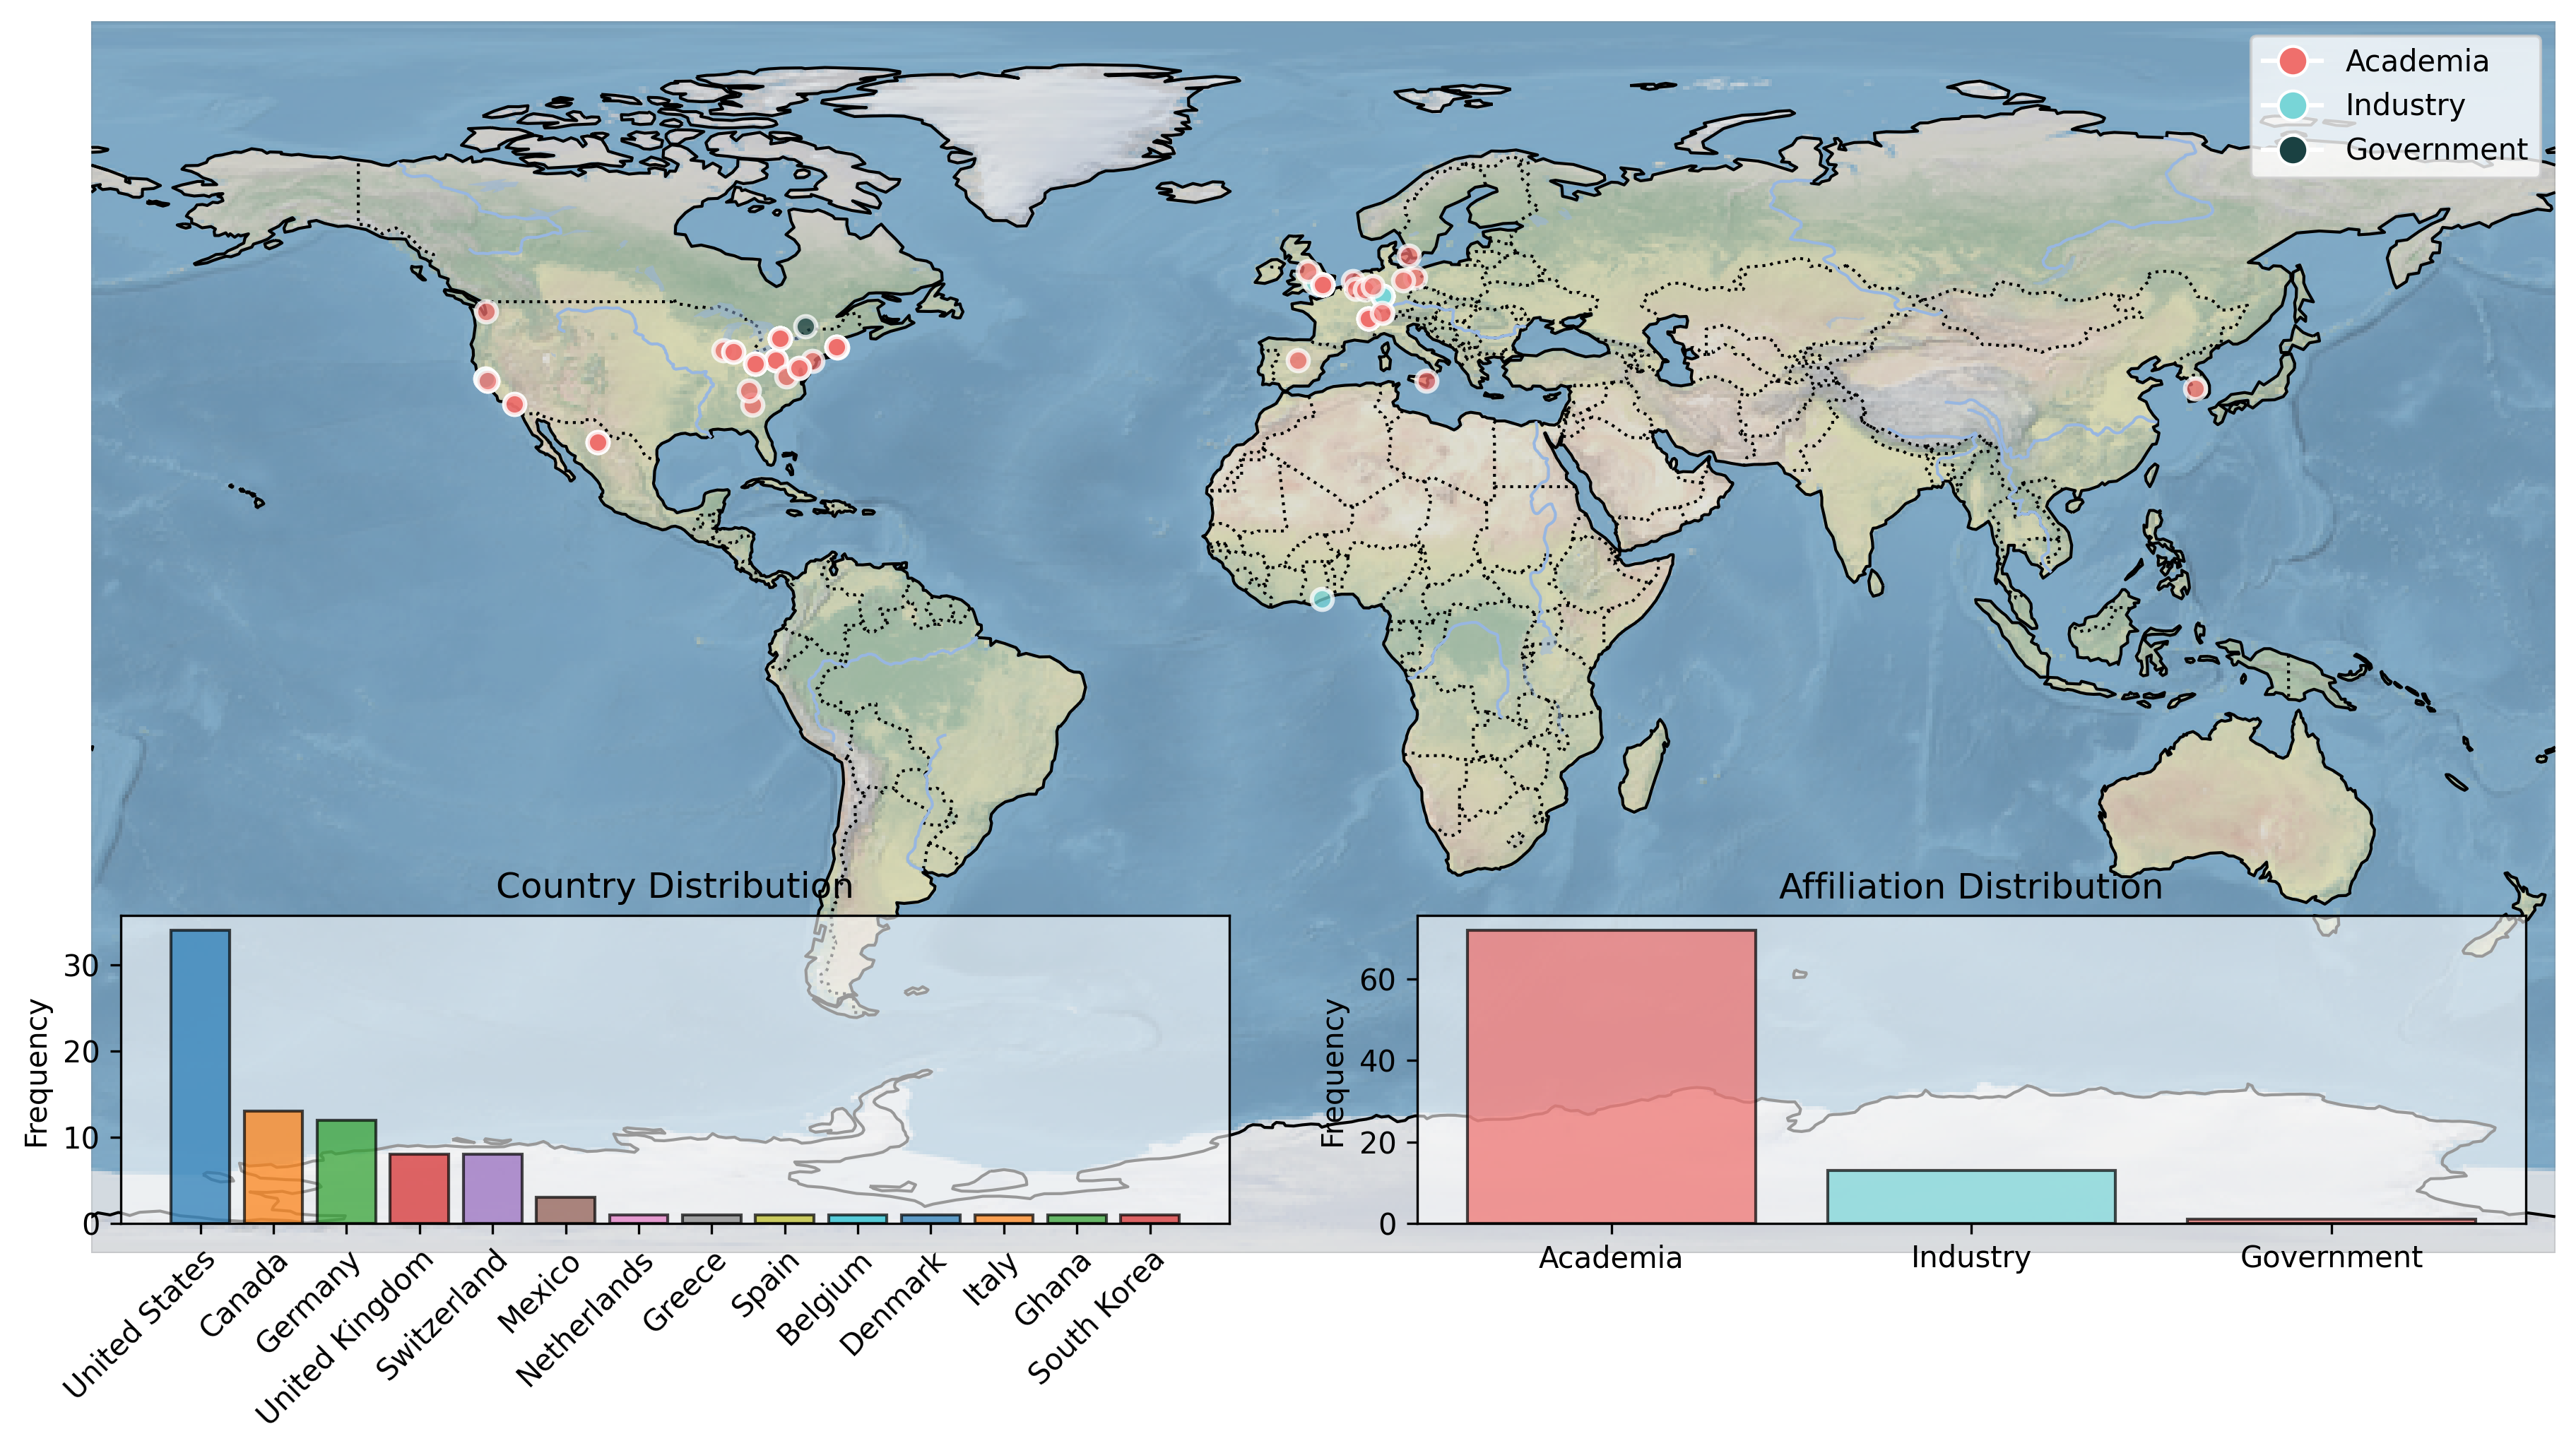
\includegraphics[width=0.95\linewidth]{latex/figures/world_map.png}
    \caption{Demographic distributions of the participating teams and their affiliations. The hackathon supported 129 participants across 60 academic, industry, and government organizations located in 59 cities, 19 countries, and 4 continents. \label{fig:map} }
\end{figure*}




% \begin{table*}[]
% \caption{List of projects and project types, with links to corresponding website project pages, repositories, videos, and social media posts.} \label{tab:projects} \setlength{\extrarowheight}{0.4em} \begin{tabularx}{\textwidth}{>{\centering\arraybackslash}p{1cm} X >{\centering\arraybackslash}X} \toprule \# & Project Name & Links \\ \midrule \href{https://example.com}{\#1} & Project A & \href{https://github.com/example}{\faGithub} \, \href{https://youtube.com}{\faVideo} \, \href{https://twitter.com}{\faTwitter} \tabularnewline \href{https://example.com}{\#2} & Project B & \href{https://github.com/example}{\faGithub} \, \href{https://youtube.com}{\faVideo} \, \href{https://linkedin.com}{\faLinkedin} \tabularnewline \href{https://example.com}{\#3} & Project C & \href{https://github.com/example}{\faGithub} \, \href{https://youtube.com}{\faVideo} \, \href{https://twitter.com}{\faTwitter} \tabularnewline \bottomrule \end{tabularx} 
% \end{table*} 


\section{Prior Materials-focused Hackathons}

\cite{jablonka_14_2023, l.ferguson_conference_2019, mulholland_hackathon_2015, sparks_insights_2024}

\section{Hackathon Details and Setup}

Participants were provided with various resources to prepare for the hackathon – this included GitHub classroom assignments with automated feedback, application- and theory-focused videos and tutorials, Python refresher materials, and a list of tools to consider using during the hackathon (\cref{fig:preparation}).

\begin{figure*}
    \centering
    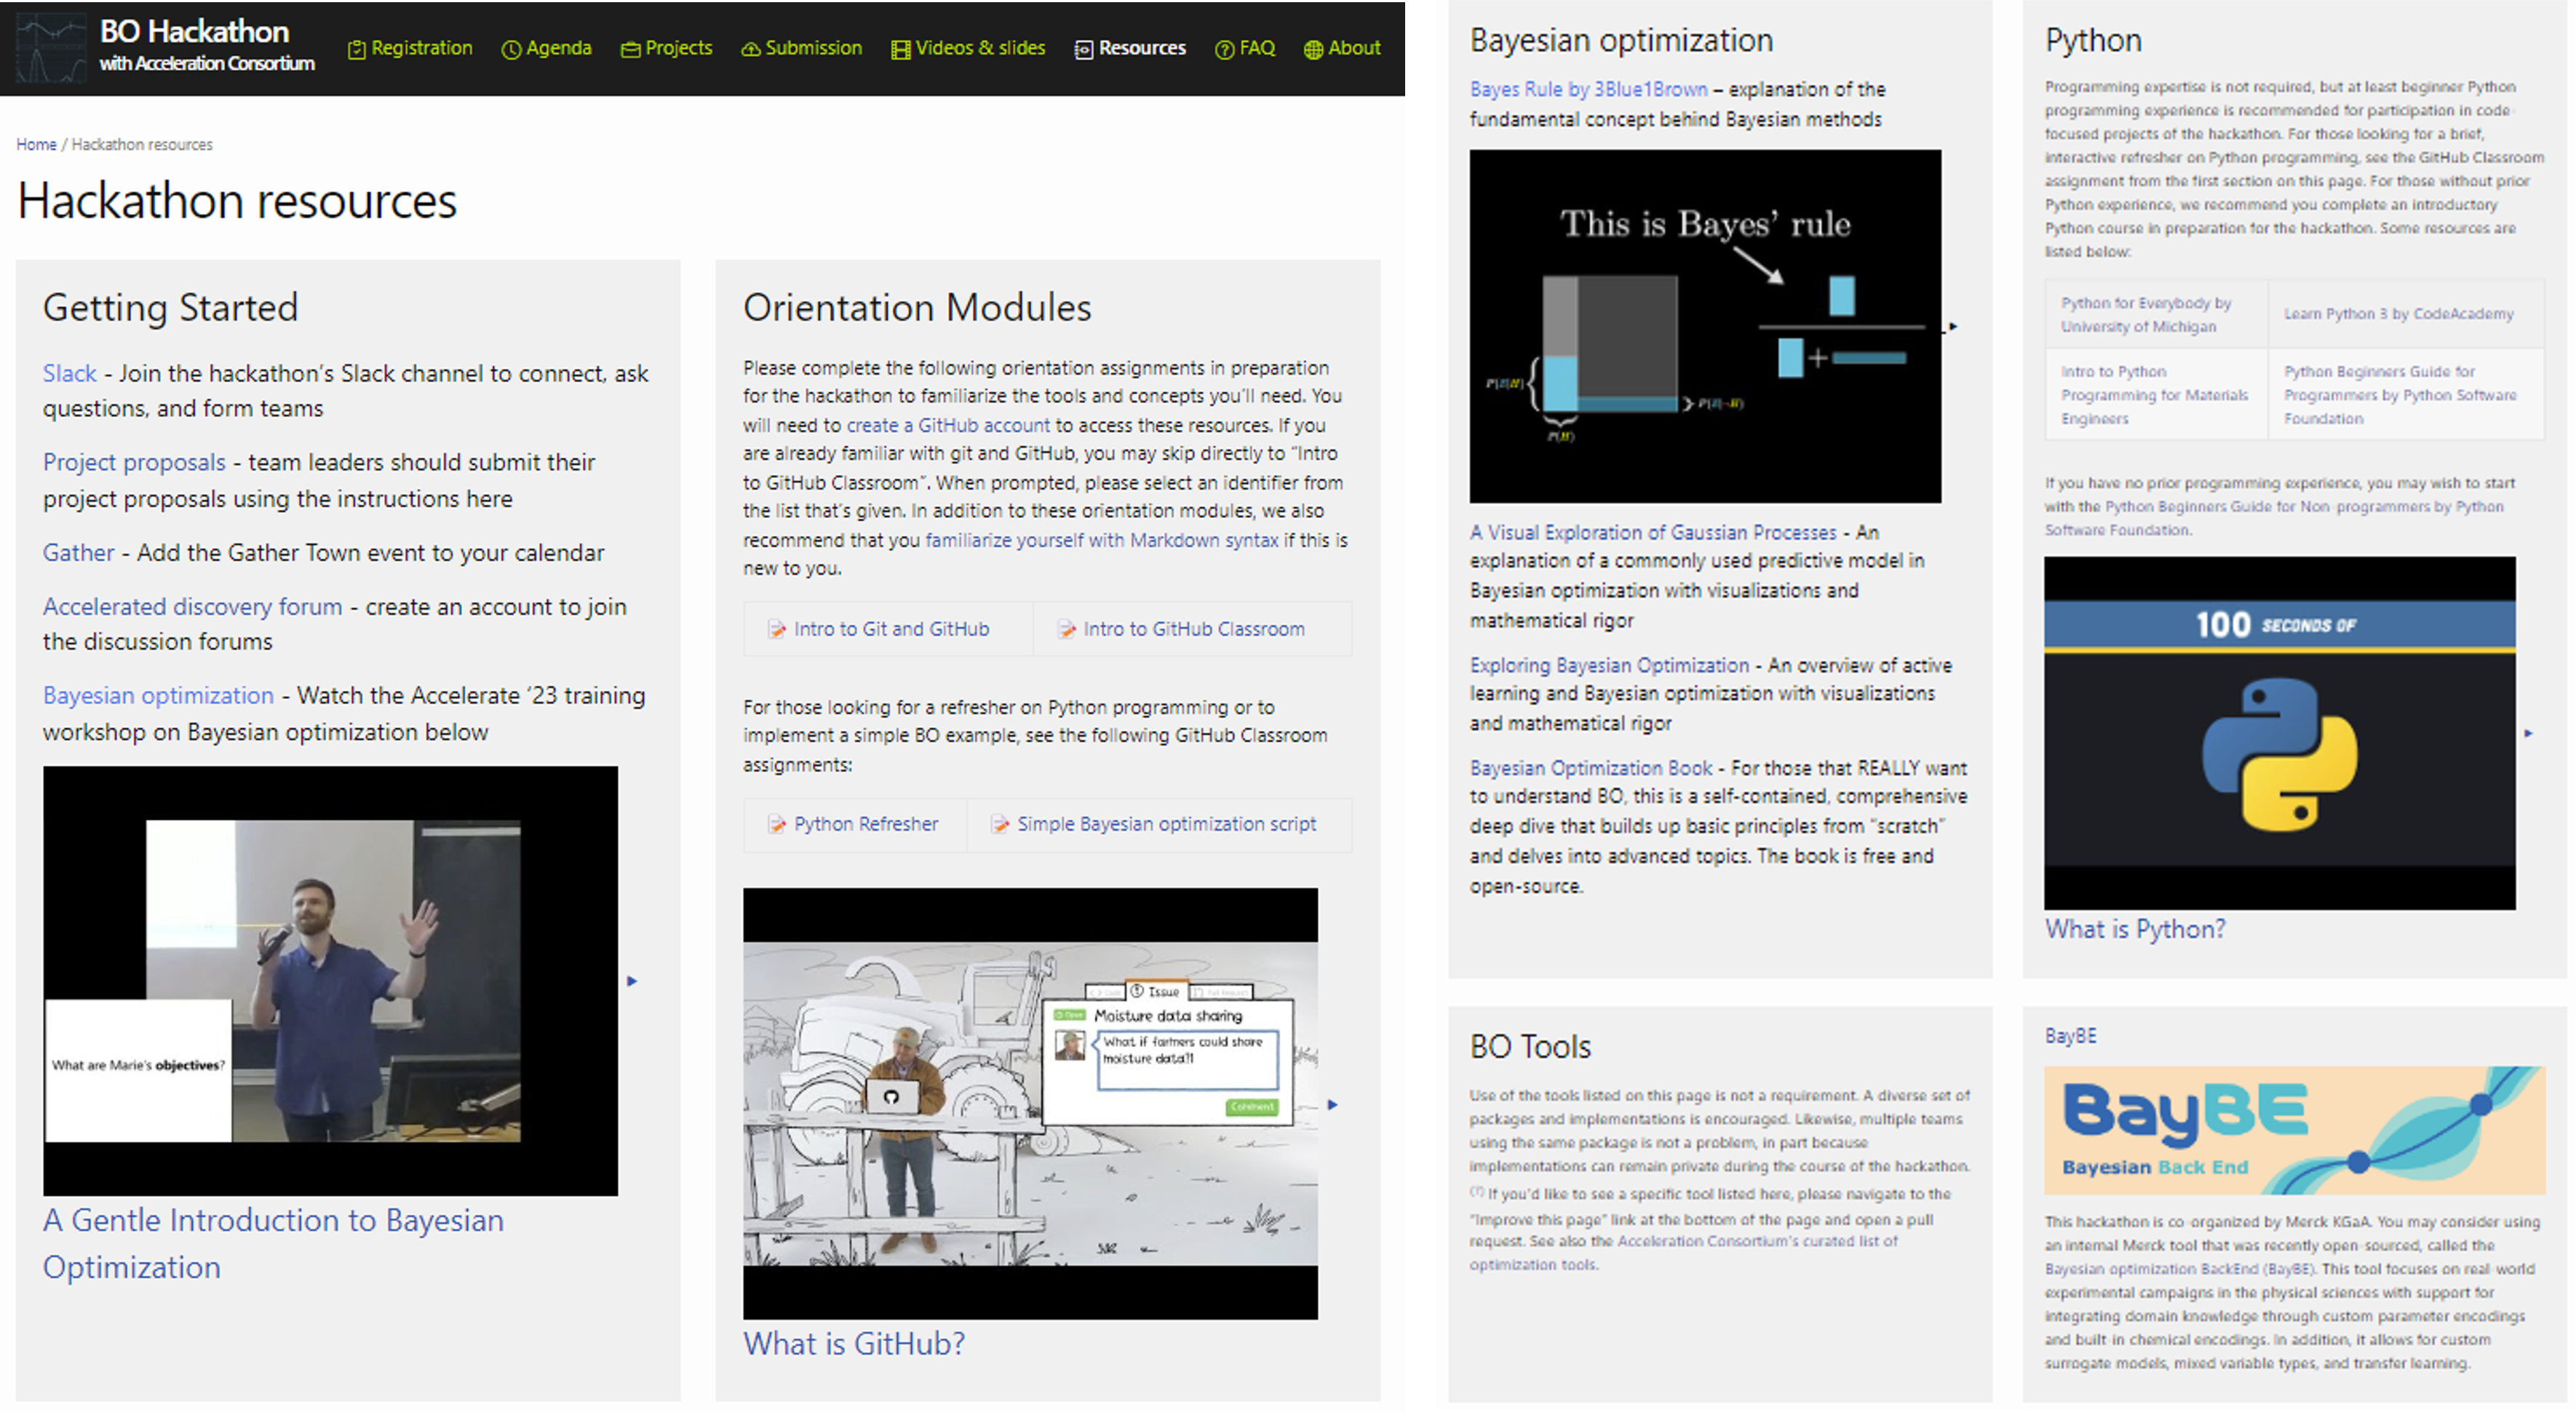
\includegraphics[width=0.98\linewidth]{latex/figures/preparation.png}
    \caption{A snapshot of \href{https://ac-bo-hackathon.github.io/resources/}{resources listed on the hackathon webpage} such as hackathon orientation, intro to \gls{bo}, and a Python refresher assignment. These resources prepared participants to maximize their time during the two-day synchronous portion of the hackathon and helped level the playing field for participants with varied backgrounds and skill levels.}
    \label{fig:preparation}
\end{figure*}

One of the unique aspects of this event is that it was hosted in Gather Town, a sort of union between traditional video conferencing software and retro arcade-style avatars and virtual spaces (\cref{fig:gathertown}). Participants create a custom avatar and maneuver in a two-dimensional space. The videos and audio of other participants appear and become audible when nearby, and fade out when far away, simulating an in-person experience. At the beginning of the hackathon, all participants gathered to listen to keynotes in realtime, which were broadcasted via YouTube live and embedded into the Gather Town space. The videos were then \href{https://ac-bo-hackathon.github.io/videos-slides/}{made available on the hackathon website}, which collectively garnered approximately 1600 views within two months. After the keynotes, teams were assigned tables in breakout rooms, each with a whiteboard. Individual tables were assigned as "private spaces" which isolated the shared audio and video within each space. This had a number of advantages for collaboration within and across teams.

\begin{figure*}
    \centering
    \includegraphics[width=0.95\linewidth]{latex/figures/gathertown.png}
    \caption{Gather town \href{https://ac-bo-hackathon.github.io/videos-slides/}{keynote} room (left), custom avatars (top-right), and an example of a breakout room for teams (bottom-right). Keynotes were broadcasted in realtime to participants via an embedded YouTube livestream. Use of Gather Town helped level the playing field for teams who were in physically separate locations and made it easier for facilitators and other teams to have more natural "check-ins" with other projects.}
    \label{fig:gathertown}
\end{figure*}


The hackathon concluded with a project showcase accompanied by crowdsourced judging within a "poster room" (\cref{fig:poster}).

\begin{figure*}
    \centering
    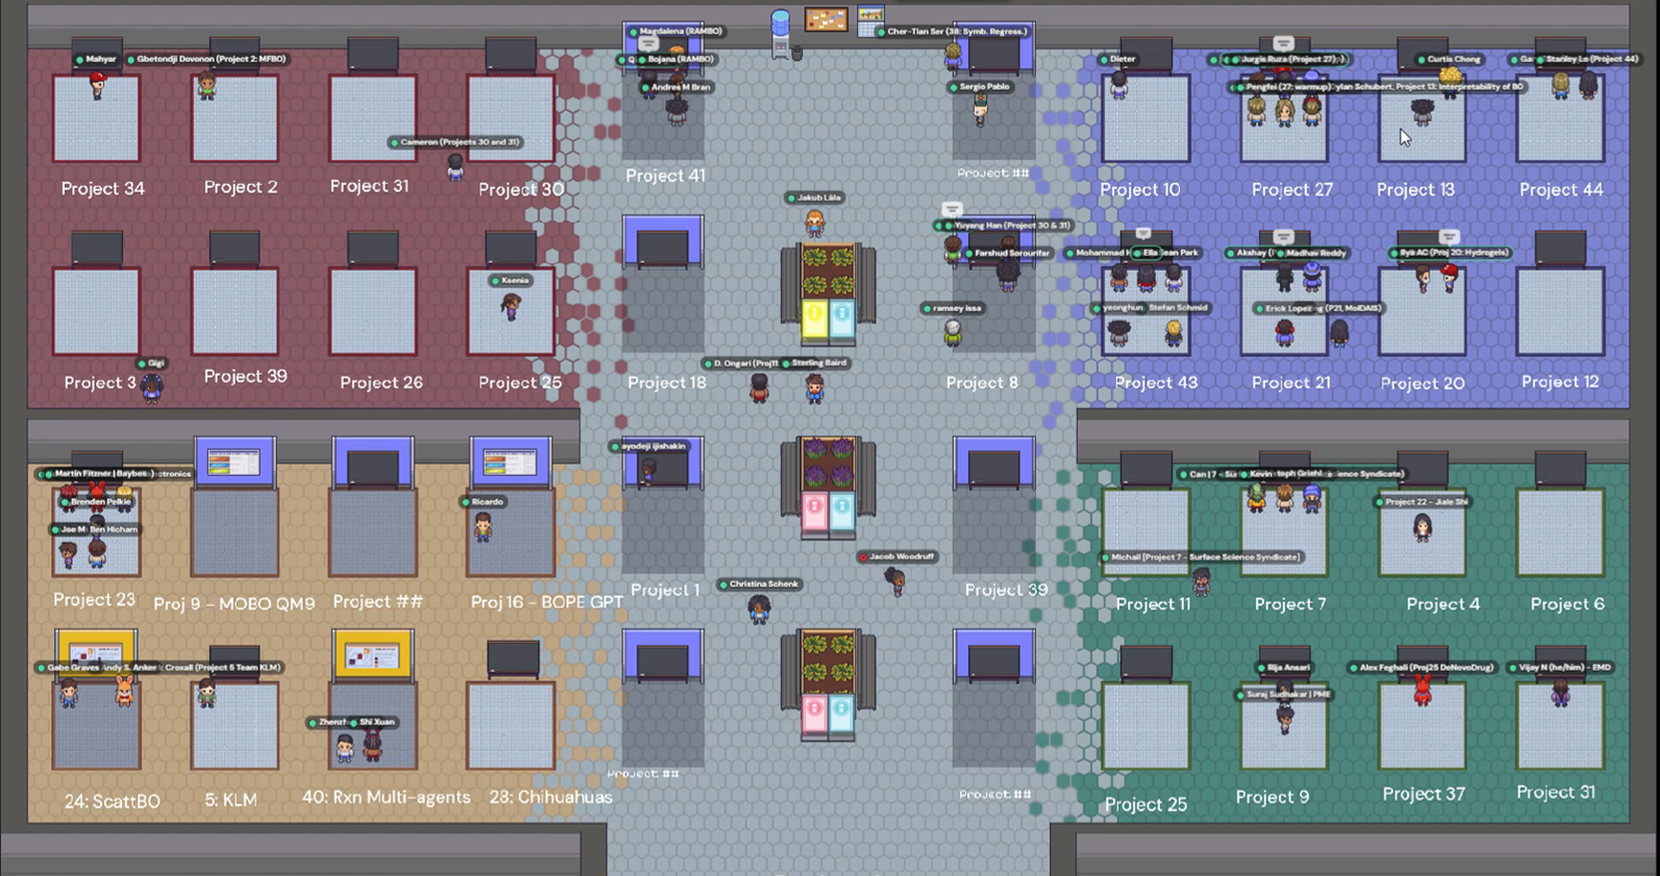
\includegraphics[width=0.95\linewidth]{latex/figures/posters.png}
    \caption{The synchronous portion of the hackathon concluded with a poster session and community judging. One participant noted that "it almost felt like a real poster session."}
    \label{fig:poster}
\end{figure*}

Community judging occurred via \href{https://github.com/anishathalye/gavel}{Gavel}, an automated pairwise comparison judging system. Use of this system helped to improve fairness, scalability, and accuracy by having judges compare projects relative to each other rather than assigning subjective numerical scores (for example, "rate your pain on a scale from 1 to 10, where 10 is the worst possible pain you can imagine"). The approach of pairwise judging reduces bias, allows for handling large competitions efficiently, and produces high-quality rankings using statistical models with dynamic assignments to judges to maximize information gain. It has been successfully used at HackMIT and other events to streamline judging and enhance transparency and credibility.

The corresponding Gavel web app was hosted on Heroku according to directions in the Gavel repository. Individualized links were distributed to judges via email using Gavel's SendGrid integration. Collectively, 35 judges cast 319 votes.



% \clearpage

\begin{longtable*}{>{\centering\arraybackslash}p{1.5cm} @{\hspace{0.4cm}} >{\raggedright\arraybackslash}p{11cm} @{\hspace{1.5cm}} >{\raggedright\arraybackslash}p{2.5cm}}
\caption{List of projects with links to GitHub, Social Media, and Video. Project pages on the hackathon website are available at \url{https://ac-bo-hackathon.github.io/projects/}.} \label{tab:projects} \\
% \toprule
% \textbf{Proj. \#} & \textbf{Project Name} & \textbf{Links} \\
% \midrule
% \endfirsthead

\toprule
\textbf{Proj. \#} & \textbf{Project Name} & \textbf{Links} \\
\midrule
\endhead

\midrule \multicolumn{3}{r}{\textit{Continued on the next page}} \\
\midrule
\endfoot

\bottomrule
\endlastfoot

1 & Multi-objective Benchmarking of Dragonfly against BoTorch & \href{https://github.com/A-Ijishakin/Multi-Objective-BO}{\faGithub} \, \href{https://www.linkedin.com/posts/jakobzeitler_why-are-you-not-using-bayesian-optimisation-activity-7173990755407929344-wRDm?utm_source=share&utm_medium=member_desktop}{\faLinkedin} \, \href{https://www.youtube.com/watch?v=Z7YiruHv3eE}{\faVideo} \\
2 & Long-run Behaviour of Multi-fidelity Bayesian Optimisation & \href{https://github.com/jean72human/LRBMFO}{\faGithub} \, \href{https://www.linkedin.com/posts/jakobzeitler_why-are-you-not-using-bayesian-optimisation-activity-7173990755407929344-wRDm?utm_source=share&utm_medium=member_desktop}{\faLinkedin} \, \href{https://www.youtube.com/watch?v=pegJumJEOsE}{\faVideo} \\
3 & Take Your Time - Improving Optimization Performance Through Greater Investment in ACQF Optimizer Runtime & \href{https://github.com/AndrewFalkowski/TakeYourTime}{\faGithub} \, \href{https://www.youtube.com/watch?v=WkGfShRSYW4}{\faVideo} \\
4 & SimpleGPT-BO, Simplified GPT-Powered Bayesian Optimization & \href{https://github.com/AC-BO-Hackathon/project-simplegpt-bo}{\faGithub} \, \href{https://www.linkedin.com/posts/arifin-375825b9_github-ac-bo-hackathonproject-simplegpt-bo-activity-7180808952383746048-mLfu}{\faLinkedin} \, \href{https://www.youtube.com/watch?v=Qr2cz5lxM64&ab_channel=ArifinSan}{\faVideo} \\
5 & Comparing Bayesian Optimization Methods Across Multiple Hyperparameters Against Simulated "Human" Decision-making & \href{https://github.com/AC-BO-Hackathon/general-project-KLM}{\faGithub} \, \href{https://www.youtube.com/watch?v=znXZhSqFtHg}{\faVideo} \\
6 & Multi-Objective Bayesian Optimization for Transparent Electromagnetic Interference Shielding with Thin-Film Structures & \href{https://github.com/AC-BO-Hackathon/project-pitt}{\faGithub} \, \href{https://x.com/jungtaek_kim/status/1833962934021881925}{\faTwitter} \, \href{https://www.youtube.com/watch?v=RgEbcWIBDn8}{\faVideo} \\
7 & BayBE One More Time - Exploring Corrosion Inhibitors for Materials Design & \href{https://github.com/AC-BO-Hackathon/project-surface-science-syndicate}{\faGithub} \, \href{https://www.linkedin.com/posts/canozkan42_github-ac-bo-hackathonproject-surface-science-syndicate-activity-7181189184894779393-5O15/?utm_source=share&utm_medium=member_desktop}{\faLinkedin} \, \href{https://www.youtube.com/watch?v=kIRxGdwmLSY}{\faVideo} \\
8 & BO for Drug Discovery-What is the role of molecular representation? & \href{https://github.com/frankwanger/ACBO-Feat}{\faGithub} \, \href{https://www.linkedin.com/posts/fanjinwang_what-is-the-role-of-molecular-featurization-activity-7179513312722726913-oFNk/}{\faLinkedin} \, \href{https://www.youtube.com/watch?v=5f_UwsfYrc8}{\faVideo} \\
9 & Optimal MOF Selection for CO2 capture using Thompson sampling & \href{https://github.com/AC-BO-Hackathon/real-world-pme-no-hikari}{\faGithub} \, \href{https://youtu.be/l0aVZDMwIMU}{\faVideo} \\
10 & Navigating the black box of zeolite synthesis with Bayesian Optimization & \href{https://github.com/AC-BO-Hackathon/project-zeolite-synthesis-bayesian-optimisation/}{\faGithub} \, \href{https://x.com/dtrplssrs/status/1834268801115791659}{\faTwitter} \, \href{https://www.youtube.com/watch?v=4lFEUixwkE8}{\faVideo} \\
11 & BlendDS - An intuitive specification of the design space for blends of components & \href{https://github.com/danieleongari/blends}{\faGithub} \, \href{https://www.linkedin.com/feed/update/urn:li:activity:7181199576073154560/}{\faLinkedin} \, \href{https://www.youtube.com/watch?v=HASa3tFLZoI}{\faVideo} \\
12 & Robust GPs for Sustainable Concrete via Bayesian Optimization & \href{https://github.com/jakobzeitler/sustainable-concrete}{\faGithub} \, \href{https://www.linkedin.com/posts/jakobzeitler_why-are-you-not-using-bayesian-optimisation-activity-7173990755407929344-wRDm?utm_source=share&utm_medium=member_desktop}{\faLinkedin} \, \href{https://www.youtube.com/watch?v=jSPGCgH31Hc}{\faVideo} \\
13 & Interpretability of Bayesian Optimisation Campaigns & \href{https://github.com/jakobzeitler/interpretable-BO}{\faGithub} \, \href{https://www.youtube.com/watch?v=Cyyj9ySybZE}{\faVideo} \\
15 & Adaptive Batch Sizes for Bayesian Optimization of Reaction Yield & \href{https://github.com/jakobzeitler/interpretable-BO}{\faGithub} \, \href{https://www.youtube.com/watch?v=utnWbJsObF0}{\faVideo} \\
16 & BOPE-GPT, Preference Exploration with the curious AI chemist & \href{https://github.com/AC-BO-Hackathon/BOPE-GPT}{\faGithub} \, \href{https://www.linkedin.com/feed/update/urn:li:activity:7179505232941326337/}{\faLinkedin} \, \href{https://www.youtube.com/watch?v=AbRDOdmafB8}{\faVideo} \\
17 & Comparative Analysis of Acquisition Functions in Bayesian Optimization for Drug Discovery & \href{https://github.com/AC-BO-Hackathon/project_acquisition_functions}{\faGithub} \, \href{https://www.linkedin.com/posts/suneelbommisetty_hackathon-bayesianoptimization-acbohackathan2024-activity-7179515945390874625-mt4M}{\faLinkedin} \, \href{https://www.youtube.com/watch?v=5AjwoZtjgOc}{\faVideo} \\
18 & Investigation of Multi-Objective Bayesian Optimization of QM9 Dataset & \href{https://github.com/AC-BO-Hackathon/project-mobo-qm9}{\faGithub} \\
20 & Closed loop optimization of hydrogel formulations using dynamic light scattering & \href{https://github.com/AC-BO-Hackathon/project-optimystics}{\faGithub} \, \href{https://www.linkedin.com/posts/ilya-yakavets_closed-loop-optimization-of-hydrogel-formulations-activity-7239817503994957824-ZRVk?utm_source=share&utm_medium=member_desktop}{\faLinkedin} \, \href{https://youtu.be/Qbvq7uolQr8}{\faVideo} \\
21 & Benchmarking Molecular Descriptors with Actively Identified Subsets (MolDAIS) & \href{https://github.com/AC-BO-Hackathon/project-The_OSU_ChemEs}{\faGithub} \, \href{https://www.youtube.com/watch?v=uYXAe3sRUSo}{\faVideo} \\
22 & Chemical Similarity-Informed Earth Mover’s Distance Kernel Bayesian Optimization for Predicting the Properties of Molecules and Molecular Mixtures & \href{https://github.com/shijiale0609/BO-EMD-Materials}{\faGithub} \, \href{https://www.youtube.com/watch?v=I179UR8P054}{\faVideo} \\
23 & Reliable Surrogate Models of Noisy Data & \href{https://github.com/AC-BO-Hackathon/project-noisy-nerds}{\faGithub} \\
24 & ScattBO Benchmark - Bayesian optimisation for materials discovery & \href{https://github.com/AndySAnker/ScattBO}{\faGithub} \, \href{https://x.com/SodeAndy/status/1773474538631651769}{\faTwitter} \, \href{https://github.com/AndySAnker/ScattBO/tree/main/presentation}{\faVideo} \\
25 & Bayesian Optimized De Novo Drug Design for Selective Kinase Targeting & \href{https://github.com/alxfgh/BO-De-Novo-Drug-Design-Docking}{\faGithub} \, \href{https://www.youtube.com/watch?v=nVtTYXxG7i4}{\faVideo} \\
26 & Multiple-Context Bayesian Optimization & \href{https://github.com/AC-BO-Hackathon/project-26-multiple-context-bo}{\faGithub} \, \href{https://x.com/Scienfitz/status/1777346768105058318}{\faTwitter} \, \href{https://www.youtube.com/watch?v=wK266A0TvZ4}{\faVideo} \\
27 & How does initial warm-up data influence Bayesian optimization in low-data experimental settings? & \href{https://github.com/eltonpan/bayes-warmup}{\faGithub} \, \href{https://twitter.com/pengfeicsci/status/1776721505361248278}{\faTwitter} \, \href{https://www.youtube.com/watch?v=4gPTMaarQt0}{\faVideo} \\
28 & The Impact of Dataset Size on Bayesian Optimization, Insights from the QM9 Dataset & \href{https://github.com/AC-BO-Hackathon/Chihuahuas}{\faGithub} \, \href{https://www.youtube.com/watch?v=hvODyYejxuc}{\faVideo} \\
30 & Active learning for voltammetry waveform design & \href{https://github.com/csmova/AC_BO_Hackathon2024}{\faGithub} \, \href{https://www.linkedin.com/feed/update/urn:li:activity:7240009028523737088/}{\faLinkedin} \, \href{https://www.youtube.com/watch?v=78bKXIIB_GA}{\faVideo} \\
31 & A tutorial on ask/tell mode for Ax & \href{https://github.com/csmova/AC_BO_Hackathon2024}{\faGithub} \, \href{https://www.linkedin.com/feed/update/urn:li:activity:7240009028523737088/}{\faLinkedin} \, \href{https://www.youtube.com/watch?v=X5PDvdXoBdA}{\faVideo} \\
32 & Efficient Protein Mutagenisis using Bayesian Optimization & \href{https://github.com/AC-BO-Hackathon/project-AiChemMcGill}{\faGithub} \, \href{https://www.linkedin.com/feed/update/urn:li:activity:7182104774291460096/}{\faLinkedin} \, \href{https://www.youtube.com/watch?v=fxpDX7Wmdc0}{\faVideo} \\
33 & Bayesian Optimization for Hyperspectral Co-heritability Search & \href{https://github.com/stair-lab/bo4ag}{\faGithub} \, \href{https://x.com/AzamRuhana17114/status/1834150551111745584}{\faTwitter} \, \href{https://www.youtube.com/watch?v=mY6Empkb8L4}{\faVideo} \\
35 & Tutorial for GAUCHE - A Library for Gaussian Processes in Chemistry & \href{https://github.com/leojklarner/gauche}{\faGithub} \, \href{https://x.com/Ryan__Rhys/status/1820723528469262419}{\faTwitter} \, \href{https://x.com/Ryan__Rhys/status/1820723528469262419}{\faVideo} \\
36 & Scalable Nonmyopic Bayesian Optimization in Dynamic Cost Settings & \href{https://github.com/sangttruong/nonmyopia}{\faGithub} \, \href{https://x.com/martinakaduc/status/1814624802629693573}{\faTwitter} \, \href{https://youtu.be/CXweDiS_wbI}{\faVideo} \\
37 & The Effects of Post-Modelling Performance Metric Computation on the Efficiency of Bayesian Optimizers & \href{https://github.com/TSAndrews/EmbeddedKnowledgeBO}{\faGithub} \, \href{https://www.linkedin.com/posts/thomas-andrews-177473143_can-the-performance-of-bayesian-optimizers-activity-7183059284807593984-BHdh?utm_source=share&utm_medium=member_desktop}{\faLinkedin} \, \href{https://www.youtube.com/watch?v=kwXHoWV8g1E}{\faVideo} \\
38 & Bayesian methods in symbolic regression & \href{https://github.com/spgarcica/symbolic_test/}{\faGithub} \, \href{https://www.youtube.com/watch?v=KKxlqo15wVY}{\faVideo} \\
39 & Divide and Conquer - Local Gaussian Processes to design Covalent Organic Frameworks for Methane Deliverable Capacity & \href{https://github.com/AC-BO-Hackathon/project-localGPs_for_COF}{\faGithub} \, \href{https://twitter.com/nik_thota/status/1775947129065967898?s=61&t=awPgdgJg4JOwPB5F4uT2CQ}{\faTwitter} \, \href{https://www.youtube.com/watch?v=iog-07Ekp9g}{\faVideo} \\
40 & Optimizing Chemical Reaction Conditions with Multi-Agent Systems Using LLM and BO & \href{https://github.com/bznan/Multi_agents_BO}{\faGithub} \, \href{https://x.com/Bozhao95501764/status/1777029207857451508}{\faTwitter} \, \href{https://x.com/Bozhao95501764/status/1777029207857451508}{\faVideo} \\
41 & Retrieval Augmented Bayesian Optimization & \href{https://github.com/schwallergroup/rambo-I}{\faGithub} \, \href{https://x.com/6ojaHa/status/1773734082637095155}{\faTwitter} \, \href{https://x.com/6ojaHa/status/1773734082637095155}{\faVideo} \\
43 & Bayesian Optimization Awesome List & \href{https://github.com/materials-data-facility/awesome-bayesian-optimization}{\faGithub} \, \href{https://www.linkedin.com/posts/benblaiszik_bohackathon-activity-7178854852620427264--sgN}{\faLinkedin} \\
44 & Rank-based Bayesian Optimization & \href{https://github.com/gkwt/rank-bo}{\faGithub} \, \href{https://x.com/mistergtom/status/1777195867730038819}{\faTwitter} \, \href{https://www.youtube.com/watch?v=c84Sd2IwMAQ&ab_channel=GaryTom}{\faVideo} \\
45 & Bayesian Optimization for generality & \href{https://github.com/felix-s-k/general-optimizers}{\faGithub} \, \href{https://www.youtube.com/watch?v=wfSyIudptfc}{\faVideo} \\



\end{longtable*}




\begin{table*}[]
\caption{Ranked Projects with Team Names and Prize Distribution. To avoid incentivizing single-person teams and very large teams, both per-person and per-team limits were imposed (e.g., teams of 4 or more would have the max per-team amount divided equally rather than receive the max per-person amount).}
\label{tab:winners}
\setlength{\extrarowheight}{0.8em}
\begin{tabularx}{\textwidth}{>{\centering\arraybackslash}p{1.0cm} >{\centering\arraybackslash}p{1.5cm} >{\centering\arraybackslash}p{3cm} X >{\centering\arraybackslash}p{3cm}}
\toprule
\textbf{Rank} & \textbf{Proj. \#} & \textbf{Team Name} & \textbf{Project Name} & \textbf{Prize* (CAD)} \\ \midrule
1st  & \#23 & Noisy Nerds                & Reliable Surrogate Models of Noisy Data                                                   & 300 (1000 max)          \tabularnewline
2nd  & \#34 & BOMS Prob                  & Streamlining Material Discovery - Bayesian Optimization in Thermal Fluid Mixtures          & 150 (500 max)           \tabularnewline
3rd  & \#7  & Surface Science Syndicate  & BayBE One More Time - Exploring Corrosion Inhibitors for Materials Design                  & 75 (250 max)            \tabularnewline
4th  & \#5  & KLM                        & Comparing Bayesian Optimization Methods \ldots Against Simulated "Human" Decision-making & 40 (125 max)            \tabularnewline
5th  & \#8  & Molecular Representation   & BO for Drug Discovery - What is the role of molecular representation?                      & 40 (125 max)            \tabularnewline
6th  & \#9  & PME No Hikari              & Optimizing The CO2 Adsorption Capacity of Metal-Organic Frameworks Using Thompson Sampling  & 40 (125 max)            \tabularnewline
7th  & \#11 & BlenDS                     & BlendDS - An intuitive specification of the design space for blends of components          & 40 (125 max)            \tabularnewline
8th  & \#30 & SERO Opt                   & Active learning for voltammetry waveform design                                            & 40 (125 max)            \tabularnewline
9th  & \#43 & General Optimizers         & Bayesian Optimization for Generality                                                      & 40 (125 max)            \tabularnewline
10th & \#3  & Sparks Group               & Take Your Time - Measuring Optimization Performance as a Function of ACQF Optimizer Runtime & 40 (125 max)           \tabularnewline
\bottomrule
\end{tabularx}
\end{table*}



% Preparation for the hackathon - 111 GitHub Classroom assignments accepted

% The hackathon was designed with tips, trick, and resources from various sources, such as https://github.com/github/hackathons.


% Hosts: Acceleration Consortium, Merck KGaA



\begin{table*}[]
\caption{Project Topics for the Hackathon. See \href{https://ac-bo-hackathon.github.io/submission/}{the submission page} for more details.}
\label{tab:project_topics}
\setlength{\extrarowheight}{0.4em}
\begin{tabularx}{\textwidth}{>{\centering\arraybackslash}p{0.5cm} p{4.5cm} X}
\toprule
 & \textbf{Topic} & \textbf{Description} \\ \midrule

1 & \textbf{Apply Algorithms} & Choose an algorithm and apply it to a \href{https://huggingface.co/collections/AccelerationConsortium/optimization-benchmarks-66a44daf10de1a0335f28826}{hackathon benchmark task} \\

2 & \textbf{Develop Benchmarks} & Develop a new benchmark and add it to a suite of benchmarks \\

3 & \textbf{Create Tutorials} & Create "gentle introduction" tutorials for \href{https://ac-microcourses.readthedocs.io/en/latest/courses/data-science/overview.html}{advanced optimization topics} \\

4 & \textbf{Propose Tasks} & Propose materials tasks that \textit{can} and \textit{should} be tackled with \gls{bo} \\

5 & \textbf{General} & Other projects related to \gls{bo} for the physical sciences \\

\bottomrule
\end{tabularx}
\end{table*}

% \clearpage

\section{Projects' Key Findings}

This section provides a comprehensive summary and highlights the key findings from all project submissions.
To streamline the evaluation process, all YouTube video submissions were transcribed and analyzed using an AI agent powered by Anthropics’s \emph{claude-3-5-sonnet-20240620} with a temperature of 0.3, ensuring consistent and accurate processing.
Each transcript was then manually edited to ensure a high-quality manuscript compilation.
This automated approach enhances efficiency while maintaining a structured and objective assessment of the submissions.


\subsection*{\href{https://www.youtube.com/watch?v=Z7YiruHv3eE}{Project 1: Multi-objective Benchmarking of Dragonfly against BoTorch}}

This research project compared the performance of two BO packages, Dragonfly\cite{JMLRdragonfly} and BoTorch\cite{balandat2020botorch}, in a multi-objective optimization context. The researchers optimized the Branin-Currin test function with added noise, conducting 20 trials of BO over different random seeds. Each trial used a batch size of 1 and consisted of 20 iterations, evaluating 20 candidates per iteration. The results showed that BoTorch's acquisition functions, particularly the q-noisy expected hypervolume improvement (qNEHVI)\cite{daulton2021parallel}, outperformed Dragonfly's acquisition function. The qNEHVI acquisition function achieved the lowest log hypervolume difference on average across the trials, while Dragonfly's acquisition function struggled to surpass a randomly generated set of candidates. Visualization of the average Pareto front produced by different acquisition functions further demonstrated BoTorch's superiority, with its acquisition functions covering a larger portion of the Pareto front compared to Dragonfly. The researchers concluded that BoTorch outperformed Dragonfly within the scope of their study, but noted the need for further investigation using different batch sizes, input and output constraints, and test functions simulating chemical reactions to apply the findings to material design problems.
 \subsection*{\href{https://www.youtube.com/watch?v=pegJumJEOsE}{Project 2: Long-run Behaviour of Multi-fidelity Bayesian Optimisation}}

This research project investigates the long-term performance of multifidelity Bayesian optimization (MFBO) methods\cite{poloczek2017multi} compared to single-fidelity Bayesian optimization (SFBO) methods. The study focuses on scenarios where two fidelities are available: an accurate but expensive target fidelity that fully represents the objective, and a less accurate but cheaper low fidelity. The researchers observed that while MFBO methods initially outperform SFBO up to a budget of approximately 20, they begin to underperform beyond this point. This behavior is particularly evident with linear kernel MFBO methods, where the performance gap becomes more pronounced after a cost of around 60.The project aims to evaluate the factors contributing to the long-term issues of MFBO methods. Specifically, the researchers plan to investigate the impact of kernel choice, frequency of low fidelity queries, and acquisition function selection on MFBO performance. By analyzing these aspects, the study seeks to identify potential improvements for MFBO methods to enhance their applicability in real-life optimization tasks. The ultimate goal is to develop MFBO approaches that can maintain their performance advantage over SFBO methods in the long run, leveraging the cost-effectiveness of low fidelity queries while achieving superior optimization results.
 \subsection*{\href{https://www.youtube.com/watch?v=WkGfShRSYW4}{Project 3: Take Your Time - Improving Optimization Performance Through Greater Investment in ACQF Optimizer Runtime}}

This research project explores an enhancement to standard BO campaigns by introducing a random seed approach to improve optimization outcomes. The team from the University of Utah's Material Science and Engineering department investigated the variability in BO campaigns when starting from the same initial data points. The key innovation in this work is a custom approach to calculating the acquisition function. Instead of computing it once per iteration, as is standard in most BO methods\cite{shahriari2015taking, snoek2012practical}, the researchers calculate the acquisition function multiple times using different random seeds. They then select the highest-performing result at each iteration. This method, termed "random retries Optimizer", showed significant improvements in optimization performance, particularly in avoiding local optima. The researchers demonstrated that this approach consistently achieves near-optimal performance among the possible campaigns stemming from the initial data points. While this method requires additional computational time for the multiple acquisition function calculations, the performance gains appear to outweigh the increased computational cost. The team is continuing to investigate questions such as the trade-off between additional compute time and performance improvements, as well as how the method performs across different types of optimization problems, including simpler ones compared to the challenging example presented.
 \subsection*{\href{https://www.youtube.com/watch?v=Qr2cz5lxM64&ab_channel=ArifinSan}{Project 4: SimpleGPT-BO, Simplified GPT-Powered Bayesian Optimization}}

No summary available.
 \subsection*{\href{https://www.youtube.com/watch?v=znXZhSqFtHg}{Project 5: Comparing Bayesian Optimization Methods Across Multiple Hyperparameters Against Simulated "Human" Decision-making}}

This research project investigated the effectiveness of BO methods that mimic human experimentalist approaches in materials science\cite{muckley2023interpretable}, comparing them to traditional BO techniques and random search baselines\cite{snoek2012practical,bergstra2012random}. The study focused on three key axes: model complexity, number of features, and acquisition function. The researchers found that a simplified "human experimentalist" approach, using automated feature engineering with a linear model, three features, and an exploitative acquisition function, was competitive with more complex random forest models in terms of enhancement factor and acceleration factor. Both the simplified approach and random forest models outperformed random search. Interestingly, for linear models, increasing complexity through additional features or more exploratory acquisition functions led to decreased performance. The main conclusion was that low-dimensional, interpretable models were comparable to traditional BO methods for the datasets and hyperparameter regimes studied. The researchers suggest future work could involve comparing their results to actual human performance and improving their methodology using theoretical approaches.
 \subsection*{\href{https://www.youtube.com/watch?v=RgEbcWIBDn8}{Project 6: Multi-Objective Bayesian Optimization for Transparent Electromagnetic Interference Shielding with Thin-Film Structures}}

This research project focuses on applying multi-objective BO to design transparent electromagnetic interference (EMI) shielding using thin film structures\cite{li2022bayesian}. The primary objectives are to maximize both transmittance and shielding effectiveness simultaneously. The optimization problem involves selecting materials and thicknesses for each layer of the thin film structure, with a search space comprising 12 material choices (Ag, Al, Al$_2$O$_3$, Cr, Ni, Pd, Si$_3$N$_4$, SiO$_2$, Ti, TiN, TiO$_2$, W) and thickness ranges from 5 to 20 nm. The researchers implemented multi-objective BO using random scalarization for the acquisition function via BayesO package\cite{kim2023bayeso}. Gaussian process regression and expected improvement were employed as part of the BO framework. The results demonstrate that the multi-objective BO approach effectively identified the Pareto frontier for the two objectives of transmittance and shielding effectiveness. This suggests that the method is successful in finding optimal trade-offs between transparency and EMI shielding performance for thin film structures, which could have applications in areas such as spacecraft windows where both properties are crucial.
 \subsection*{\href{https://www.youtube.com/watch?v=kIRxGdwmLSY}{Project 7: BayBE One More Time - Exploring Corrosion Inhibitors for Materials Design}}

This research project explored the use of BO for efficiently identifying effective corrosion inhibitors in materials design. The researchers utilized the BO implementation from the BayBE package\cite{fitzner2022baybe} to evaluate its performance on multiple experimental datasets\cite{galvao2022cordata} involving different alloys, primarily aluminum-based. The study found that the choice of molecular descriptor encoding significantly impacted the optimization performance, especially for larger datasets like A1000 and A2024. The SMILES-based approach with Mordred encoding\cite{moriwaki2018mordred} outperformed the other methods for these datasets, while random sampling underperformed. Interestingly, for the A775 dataset, which had a sparse distribution of reported efficiencies and fewer data points, this trend was not observed. The researchers also explored transfer learning capabilities, using information from the A2024 alloy dataset to inform the optimization process for the A1000 dataset. This transfer learning approach outperformed the uninformed method after only 15 iterations, demonstrating its potential for accelerating the discovery of effective corrosion inhibitors in experimental settings.
 \subsection*{\href{https://www.youtube.com/watch?v=5f_UwsfYrc8}{Project 8: BO for Drug Discovery-What is the role of molecular representation?}}

This research project investigated the impact of molecular featurization methods on BO performance for guiding molecular experiments. The team explored alternatives to the commonly used connectivity-based fingerprints, aiming to determine which featurization techniques yield the best results in BO for molecular discovery.The study found that without modifying the features, MACCS\cite{durant2002reoptimization} and RDKit\cite{landrum2013rdkit} featurization methods outperformed the default options presented in previous publications. To address the high dimensionality of molecular features, the researchers employed specialized Gaussian processes and explored random forest surrogates. However, the random forest approach did not improve performance and required more computational resources. Principal Component Analysis (PCA) was successfully used to enable Gaussian processes to handle large molecular featurizations. Notably, physicochemical featurizations like RDKit and Mordred\cite{moriwaki2018mordred} outperformed the previous benchmark winner, MolDQN\cite{zhou2019optimization}. The team's findings were consistent with benchmarks in the BO library but suggested that RDKit could produce even better results than Mordred. Overall, the research highlights the importance of careful featurization selection in BO for molecular discovery, with RDKit emerging as a particularly effective option.
 \subsection*{\href{https://youtu.be/l0aVZDMwIMU}{Project 9: Optimal MOF Selection for CO$_2$ capture using Thompson sampling}}

This research project focuses on optimizing the selection of Metal-Organic Frameworks (MOFs) for carbon capture applications using BO, specifically Thompson Sampling. MOFs are nanoporous materials with high potential for carbon capture\cite{furukawa2013chemistry, heo2020metal}, but their synthesis and characterization are expensive and time-consuming\cite{desantis2017techno}. The goal was to develop an efficient method for identifying high-performing MOF candidates using a small dataset. The team employed a Gaussian Process model trained on the CRAFTED dataset\cite{oliveira2023crafted}, using both RACs features and geometric features of MOFs, with CO$_2$ uptake as the output. Thompson Sampling was used as the acquisition function to select the next best sample based on the posterior distribution, inherently performing a Bayesian update. The results showed that Thompson Sampling was twice as efficient as random sampling in identifying high-performing MOF candidates. This approach is notable for being the first application of Thompson Sampling to MOF candidate selection, and it requires no hyperparameter tuning, making it easily transferable and cost-efficient. The potential impact of this method is significant, as it could accelerate MOF design for direct air capture applications, with a goal of absorbing 30 million tons of CO$_2$, and could also be applied to post-combustion capture scenarios.
 \subsection*{\href{https://www.youtube.com/watch?v=4lFEUixwkE8}{Project 10: Navigating the black box of zeolite synthesis with Bayesian Optimization}}

This research project explores the application of BO to zeolite synthesis, a complex process with significant industrial importance. Zeolites are crystalline materials composed of interconnected silicate and aluminate tetrahedra, widely used as absorbents and catalysts\cite{dusselier2018small}. The synthesis of zeolites involves multiple parameters, including silicon and aluminum sources, organic molecules, water, temperature, and time. The process aims to achieve specific properties such as high crystallinity, large external surface area, and particular silicon-to-aluminum ratios, while also considering economic factors like synthesis temperature, duration, and ingredient concentrations\cite{mallette2024current}. The project presents a GitHub repository containing an introductory text on zeolites and their synthesis, along with a Jupyter notebook demonstrating BO applications. The notebook is divided into two main sections: the first optimizes an analytical dummy function using zeolite synthesis parameters, exploring various aspects of BO including continuous, categorical, and mixed variable types, parameter constraints, and single and multiple objectives. The second section applies BO to propose new experiments based on existing literature data. This approach aims to accelerate the traditionally time-consuming trial-and-error process of zeolite synthesis optimization, potentially reducing costs and improving efficiency in industrial applications.
 \subsection*{\href{https://www.youtube.com/watch?v=HASa3tFLZoI}{Project 11: BlendDS - An intuitive specification of the design space for blends of components}}

This project focuses on developing an interface for BO that bridges the gap between domain experts (i.e. chemists and materials scientists) and machine learning algorithms. The system allows scientists to specify experimental parameters and constraints in natural language, which is then translated into a structured dictionary format by a large language model. This dictionary is subsequently converted into a Python object that can be used for design of experiments and optimization tasks.The key feature of this interface is its ability to generate diverse trial designs for efficient sampling of the experimental space. It incorporates dimensionality reduction techniques to visualize the design space, enabling users to select the most diverse and informative trials. This approach aims to maximize the information gained from each experiment, potentially reducing the number of trials needed to reach optimal results. The project is open-source, inviting contributions and integration with existing BO frameworks.
 \subsection*{\href{https://www.youtube.com/watch?v=jSPGCgH31Hc}{Project 12: Robust GPs for Sustainable Concrete via Bayesian Optimization}}

This project introduces Robust Gaussian Processes (Robust GPs)\cite{altamirano2023robust} to the concrete sciences experiments with Bayesian optimization campaigns. The research addresses the common issue of outliers in concrete science experiments by applying Robust GPs to account for these anomalies. The project provides a tutorial and accompanying code in a GitHub repository, demonstrating how to implement Robust GPs in this specific context. The study utilizes a dataset provided by Meta\cite{ament2310sustainable}, which includes input variables and a target variable representing concrete strength. Initial data analysis reveals potential outliers in the strength variable, with values between 2 and 2,000. The researchers then apply Robust GP to this dataset, achieving good predictive performance. The project culminates in demonstrating how to obtain Bayesian recommendations using the Robust GP as a surrogate model, providing a practical approach for optimizing concrete mixtures while accounting for experimental outliers.
 \subsection*{\href{https://www.youtube.com/watch?v=Cyyj9ySybZE}{Project 13: Interpretability of Bayesian Optimisation Campaigns}}

This research project focused on developing novel methods for interpreting Bayesian Optimization campaigns by incorporating the temporal component often neglected in end-of-campaign analyses. The study utilized data from a self-driving lab experiment aimed at optimizing the conductivity of a coating. The researchers recreated the Gaussian Process (GP) model employed in the original experiment, training it on subsets of data to simulate mid-campaign conditions. Two primary methods were investigated: First, cross-sections of the GP model were taken at various stages of the campaign, holding all but one feature constant. This approach revealed that closer nozzle distances produced better results, aligning with prior beliefs and serving as a potential mid-campaign sense check to validate model alignment with previous experimentation. The second method involved predicting the error of the next sample based on the model trained on data collected up to that point. This analysis showed that performance improvement plateaued around the time the optimal sample was produced, suggesting its potential use as an early stopping criterion if error is monitored throughout the campaign.The research demonstrates the value of incorporating temporal analysis in Bayesian Optimization campaigns, offering insights that could enhance decision-making during experiments. The cross-sectional approach provides a means to validate model behavior against prior knowledge, while the error prediction method could inform stopping criteria, potentially improving efficiency in optimization processes. These techniques offer promising avenues for real-time interpretation and guidance in Bayesian Optimization experiments, particularly in self-driving lab contexts.
 \subsection*{Project 14: Bayesian optimization of likely negative candidates in imbalanced biological datasets}


 \subsection*{\href{https://www.youtube.com/watch?v=utnWbJsObF0}{Project 15: Adaptive Batch Sizes for Bayesian Optimization of Reaction Yield}}

This research project investigates the optimization of batch sizes in BO for chemical reaction yield optimization. The study focuses on determining the optimal batch size (Q) at each step of the BO process, considering both smaller and larger batch sizes. The researchers examine how Q impacts the cost of retraining models, such as large language models, and how it relates to additional experimentation overhead. The project findings indicate that the optimal Q depends on a trade-off between model retraining time and additional experimentation overhead. For a fixed batch size, the researchers observed two minima at Q=3 and Q=7, reflecting the relative importance of Q in different scenarios. With very large batch sizes, the retraining cost had minimal impact on the overall experimental overhead, while experimentation overhead had a significant influence. The study also explored adaptive batch sizing strategies, decreasing batch sizes when performance was good and increasing them as the surrogate model became more trustworthy. The researchers conclude that batch sizes have a crucial effect on BO efficiency in real-world settings, and adaptive batch sizes could effectively balance the trade-off between model retraining and batch sampling effectiveness.
 \subsection*{\href{https://www.youtube.com/watch?v=AbRDOdmafB8}{Project 16: BOPE-GPT, Preference Exploration with the curious AI chemist}}

This research project focused on optimizing the Fischer-Tropsch synthesis process\cite{mahmoudi2017review}, which converts syngas into biofuel hydrocarbons. The optimization problem on the dataset\cite{lozano2008single,chakkingal2022multi} involved four input variables (space time, syngas ratio, temperature, and pressure) and four output variables (carbon conversion, selectivity, methane to paraffins, and olefins). The researchers proposed a novel approach using preferential BO\cite{lin2022preference} with large language models (LLMs) to prioritize outputs based on stakeholder preferences. The methodology employed the typical BO process powered by BoTorch, using Expected Utility as the acquisition function. However, the innovation lay in using an LLM (specifically GPT-4) to perform pairwise comparisons for output prioritization. The results showed that outputs exhibited well-defined optima trade-offs and some degree of monotonicity, which was important for preferential BO. The researchers tested three objective scenarios: optimizing all outputs equally, maximizing only CO conversion, and maximizing three objectives while minimizing olefins. For the first two objectives, the LLM-based preferential BO performed similarly to traditional utility function-based methods. However, for the third, more complex objective, the LLM approach performed worse than the utility function method and only slightly better than random exploration, suggesting limitations in the LLM's ability to handle complex optimization scenarios. The project also included the development of an interactive application for visualizing BO results and running live optimizations.
 \subsection*{\href{https://www.youtube.com/watch?v=5AjwoZtjgOc}{Project 17: Comparative Analysis of Acquisition Functions in Bayesian Optimization for Drug Discovery}}

This project investigates the application of BO techniques directly on molecular fingerprints for drug discovery, focusing on comparing different surrogate models, acquisition functions and small, diverse, unbalanced, and noisy datasets\cite{bellamy2022batched}. The researchers used the LD50 dataset from PTDC with SMILES encodings\cite{wu2018quantitative,chen2021algebraic}, which were transformed into ECFP fingerprints\cite{rogers2010extended}, creating a 2048-dimensional feature space. Two surrogate models were examined: Gaussian Processes (GP) and Random Forests (RF). The results showed that in this high-dimensional space, Random Forests with uncertainties evaluated as variance between different trees achieved expected performance across all acquisition functions, significantly outperforming random selection. In contrast, Gaussian Processes failed to perform well, likely due to the challenges posed by the high-dimensional space ($2\textasciicircum{}{2048}$ possible combinations) and the relatively small dataset of only 7,000 data points. The researchers concluded that machine learning models, particularly Random Forests with various acquisition functions, perform well when dealing with high-dimensional molecular fingerprint spaces, demonstrating their potential for drug discovery applications with certain selection biases.
 \subsection*{Project 18: Investigation of Multi-Objective Bayesian Optimization of QM9 Dataset}


 \subsection*{Project 19: Quantum Bayesian Optimization for Automatic Chemical Design}


 \subsection*{\href{https://youtu.be/Qbvq7uolQr8}{Project 20: Closed loop optimization of hydrogel formulations using dynamic light scattering}}

This research project proposes a self-driving lab approach to optimize hydrogel formulations using BO and automated characterization techniques. The study aims to address the challenge of creating hydrogels with specific properties for applications such as cell culture, tissue engineering, drug delivery, and agriculture. The proposed workflow utilizes an open-source liquid handling robot to mix hydrogel formulations in a 96-well plate, followed by cross-linking using various methods (LED array, heating module, or time). The key innovation is the use of Dynamic Light Scattering (DLS)\cite{stetefeld2016dynamic} for automated characterization of gelation and viscoelastic properties, which can measure gel stiffness up to 10 kilopascals. This DLS method is implemented using a plate reader specifically designed for 96-well plates, enabling high-throughput analysis. The resulting property data is then fed into a Bayesian Optimizer to determine the next set of formulations and processing parameters to test. This approach aims to efficiently explore the complex relationship between hydrogel formulation parameters and their resulting properties, potentially accelerating the development of custom hydrogels for specific applications in biological research and improving data availability and reliability in the field.
 \subsection*{\href{https://www.youtube.com/watch?v=uYXAe3sRUSo}{Project 21: Benchmarking Molecular Descriptors with Actively Identified Subsets (MolDAIS)}}

This research presents a novel approach called MOLDES (Molecular Descriptors with Actively Identified Subspaces) for molecular property optimization. The method addresses the challenge of optimizing molecules in high-dimensional spaces by using molecular descriptors - sets of rotationally and translationally invariant calculations performed on molecular graphs - coupled with active subspace identification. MOLDES employs a sparse axis-aligned subspace Gaussian Process prior, which actively learns an encoding while performing Bayesian optimization. Recent works\cite{sorourifar_accelerating_2024,maus_local_2023} are increasingly turning towards active encoding of molecular feature spaces. The researchers evaluated MOLDES on three case studies: experimental lipophilicity (4,200 compounds), log P optimization benchmark (250,000 molecules), and power conversion efficiency from the Harvard Clean Energy Project (30,000 compounds). In all cases, MOLDES demonstrated superior performance compared to other optimizers, particularly in larger datasets. For the log P optimization, MOLDES consistently found the optimal molecule within 100 iterations. The method also showed strong performance in constrained optimization problems, often achieving the best-case scenario and maintaining a favorable worst-case scenario compared to other methods. Overall, MOLDES proved efficient in identifying high-performing molecules in low-data regimes, offering a promising approach for molecular property optimization tasks.
 \subsection*{\href{https://www.youtube.com/watch?v=I179UR8P054}{Project 22: Chemical Similarity-Informed Earth Mover’s Distance Kernel Bayesian Optimization for Predicting the Properties of Molecules and Molecular Mixtures}}

This research project focuses on developing chemical similarity-informed distance functions and kernels for explainable Bayesian optimization, specifically targeting the prediction of properties for molecular mixtures. The researchers propose a novel approach that bypasses the need for embedding vectors by directly providing pairwise distances between data points in the kernel function of a Gaussian Process (GP) model\cite{moss_gaussian_2020}. The project introduces the Earth Mover's Distance (EMD) kernel\cite{hargreaves_earth_2020} into the GP framework to calculate pairwise distances between mixtures based on individual component distances. This method was tested for predicting yields of binary reactant mixtures, demonstrating high chemical resolution in mixture analysis. The results show that the EMD kernel achieves accurate yield predictions with narrow distributions for both high and low-yield cases, indicating improved performance in distinguishing between different mixture compositions. By incorporating smooth distance metrics, the researchers successfully extended Bayesian optimization techniques from pure components to molecular mixtures, potentially enhancing the efficiency and interpretability of materials property prediction in complex chemical systems.
 \subsection*{Project 23: Reliable Surrogate Models of Noisy Data}


 \subsection*{\href{https://twitter.com/SodeAndy/status/1773474538631651769}{Project 24: ScattBO Benchmark - Bayesian optimisation for materials discovery}}

This project presents ScattBO, a Python-based benchmark that simulates a self-driving laboratory (SDL) for materials discovery. A self-driving laboratory is an autonomous platform that conducts machine learning-selected experiments to achieve a user-defined objective, such as synthesizing a specific material\cite{szymanski_autonomous_2023}. The benchmark addresses the challenge that such SDLs can be expensive to run, making intelligent experimental planning essential, while only a few people have access to real SDLs for materials discovery. ScattBO provides an in silico simulation of an SDL where, based on synthesis parameters, the benchmark 'synthesizes' a structure, calculates the scattering pattern\cite{johansen_gpu-accelerated_2024}, and compares it to the target structure's scattering pattern. The benchmark acknowledges that scattering data may not be sufficient to conclusively validate that the target material has been synthesized\cite{leeman_challenges_2024}, but can include other types of data as long as they can be simulated. This makes it currently challenging to benchmark Bayesian optimization algorithms for experimental planning tasks in SDLs, and ScattBO fills this gap by providing an accessible simulation environment.
 \subsection*{\href{https://www.youtube.com/watch?v=nVtTYXxG7i4}{Project 25: Bayesian Optimized De Novo Drug Design for Selective Kinase Targeting }}

This project focused on incorporating Bayesian optimization to guide de novo drug design, specifically targeting growth factor receptors for cancer therapeutics. The team built upon the DOCKSTRING paper, Python library, and dataset\cite{garcia_dockstring_2022}, using a Gaussian process with a Matérn kernel on Morgan fingerprint representations. They employed a graph genetic algorithm to generate SMILES strings guided by the Bayesian optimization output. The researchers explored both selective and promiscuous binding scenarios. For selective binding, they optimized for binding to FGFR1 while penalizing overbinding to other growth factor receptors relative to their median. For promiscuous binding, they maximized the maximum binding affinity across multiple receptors. They found that a sigmoidal penalty function was more effective than simple absolute differences when optimizing against multiple proteins. The team also incorporated a drug-likeness measure (QED)\cite{bickerton_quantifying_2012} as a penalty in the optimization process, though its effect was limited. Due to time and resource constraints, the project was unable to extensively explore the chemical space or use more accurate binding affinity calculations beyond docking. The authors suggest that future work could incorporate known unknowns through an evasion process, further optimize selective binding, and compare different molecular representations.
 \subsection*{\href{https://www.youtube.com/watch?v=wK266A0TvZ4}{Project 26: Multiple-Context Bayesian Optimization}}

This project focused on exploring multiple context Bayesian optimization using the BAYO code, a Bayesian backend package built on BoTorch with additional features. The primary aim was to investigate transfer learning capabilities by incorporating data from existing campaigns into new optimization tasks.The researchers examined both analytical functions (like the Hartmann 3D function) and real-world data (direct arylation reaction dataset) to assess the effectiveness of transfer learning in Bayesian optimization. They introduced noise, scaling, shifting, and negation to the analytical functions to simulate realistic scenarios. The results demonstrated that using a small percentage (1-25\%) of existing data significantly improved optimization performance compared to the baseline without transfer learning. Interestingly, they found that using larger amounts of data (50-100\%) did not necessarily lead to better results and in some cases performed worse than the baseline. The team also explored clustering the existing data and using cluster centroids as source data, which proved effective. For the real-world direct arylation dataset, they analyzed correlations between different reaction temperatures and observed that small amounts of transfer data (1-10\%) substantially improved the Bayesian optimization campaign. Overall, the project highlighted the potential of transfer learning in Bayesian optimization while emphasizing that careful selection of the amount and type of transfer data is crucial for optimal performance.
 \subsection*{\href{https://www.youtube.com/watch?v=4gPTMaarQt0}{Project 27: How does initial warm-up data influence Bayesian optimization in low-data experimental settings?}}

This research project investigated the influence of warm-up sampling methods and dataset sizes on property optimization in low data regimes, specifically focusing on molecular property prediction. The team used the QM9 dataset\cite{ramakrishnan_quantum_2014} and selected band gap as the optimization target. They compared two chemically-inspired sampling methods for the warm-up dataset: Morgan fingerprints and MolFormer language model fingerprints. The researchers also referenced the GDB-17 chemical universe database\cite{ruddigkeit_enumeration_2012} in their background work. The researchers performed dimensionality reduction on the fingerprints using PCA, projecting them into a 2D space for sampling. They conducted experiments to analyze how the warm-up dataset size affects optimization results. The most significant finding was the comparison between Morgan fingerprints and MolFormer fingerprints at a constant data regime of 50 data points. The results showed that MolFormer fingerprints substantially outperformed Morgan fingerprints, suggesting that pre-trained models on large chemical spaces can potentially improve model optimization rates. This study aims to initiate broader discussions on how dataset sizes and sampling methodologies impact final optimization tasks in molecular property prediction.
 \subsection*{\href{https://www.youtube.com/watch?v=hvODyYejxuc}{Project 28: The Impact of Dataset Size on Bayesian Optimization, Insights from the QM9 Dataset}}

No summary available.
 \subsection*{Project 29: A Bayesian Approach to Predict Solubility Parameters}


 \subsection*{\href{https://www.youtube.com/watch?v=78bKXIIB_GA}{Project 30: Active learning for voltammetry waveform design}}

This research project focused on using Bayesian Optimization to optimize voltammetry waveforms for sensor performance testing. The researchers employed the scikit-optimize package to implement a human-in-the-loop optimization process, allowing for pauses between optimization iterations to conduct laboratory experiments.The study encoded a four-step pulse waveform into a continuous parameter space for the optimization model. The process began with six randomly generated initial waveforms, which were tested in the lab to obtain performance metrics. These results were used to initialize a Gaussian process model. The optimization then proceeded in batches, with the model suggesting the next best waveforms to test based on previous results. The researchers conducted four total batches, updating the model after each laboratory testing phase. Progress plots were generated to visualize the improvement in sensor error across batches, demonstrating the effectiveness of the approach in finding optimal waveform parameters. The study also explored the interactions between model parameters and the performance metric across multiple dimensions, providing insights into the complex relationship between waveform characteristics and sensor performance.
 \subsection*{\href{https://www.youtube.com/watch?v=X5PDvdXoBdA}{Project 31: A tutorial on ask/tell mode for Ax}}

This project focuses on utilizing the open-source package AXS for Bayesian optimization in an asynchronous, human-in-the-loop experimental setting, particularly applied to voltammetry. The researchers developed custom figures and explanations to elucidate the complex interactions within the AXS package, emphasizing its user-friendly nature while acknowledging its potential complexity.The study explores various aspects of the optimization process, including strategy selection, surrogate model choice, and search space definition. It demonstrates two primary approaches: a "cold start" scenario, where optimization begins with no prior data, and a "warm start" scenario for situations with existing experimental data. For the cold start, the researchers showcase the use of sequence generators like Sobol sequences and random generators to initialize the optimization campaign. The project also highlights the package's ability to handle real-world experimental constraints, such as marking broken electrodes to exclude them from future suggestions. In the warm start scenario, the researchers detail the process of translating existing experimental workflows into the AXS framework, emphasizing the package's automatic tracking of experiments, results, and parameters. The study also notes the inclusion of visualization tools within AXS, though these are not described in detail.
 \subsection*{\href{https://www.youtube.com/watch?v=fxpDX7Wmdc0}{Project 32: Efficient Protein Mutagenisis using Bayesian Optimization}}

This research project explored the application of Bayesian optimization to protein mutagenesis, specifically aiming to optimize protein binding affinity to fentanyl for potential use in biosensors. The team utilized a pre-trained BERT language model, published by Andrew E. Bial, which predicts ligand binding to proteins based on amino acid sequences and SMILES strings. The methodology involved using Bayesian optimization to iteratively select positions and amino acids for mutation, starting with a protein that already had affinity to fentanyl, published by Lisa Mu Banks. The researchers focused on residues within 5 angstroms of the ligand as potential mutation sites.The team compared their Bayesian optimization approach to a baseline using random mutations. They analyzed the resulting mutations using PyRosetta's mutagenesis tool to identify potential new positive interactions and clashes that could alter protein conformation. The structural changes were further investigated using AlphaFold. While the project demonstrated the potential of Bayesian optimization for protein engineering, it was limited by its short two-day duration, suggesting room for further improvements and more extensive analysis.
 \subsection*{\href{https://www.youtube.com/watch?v=mY6Empkb8L4}{Project 33: Bayesian Optimization for Hyperspectral Co-heritability Search}}

This research project focuses on applying Bayesian Optimization (BO) to the field of crop genetics, specifically for selecting optimal proxy data to train genomic prediction models. The goal is to identify resilient crops that can withstand factors like pests and climate change. The study uses coheritability as a measure to determine the best proxy traits for desired traits, treating it as a black-box optimization problem.The researchers compared various BO methods using Gaussian Processes (GPs) against random search for four different desired traits. Surprisingly, they found that all BO methods performed similarly to random search. However, a pre-trained probabilistic model with a mixed multitask kernel outperformed standard BO approaches, identifying better proxy data more quickly. The study concludes that Gaussian Processes may not be the optimal choice for this particular problem, challenging the common use of Matérn kernels and GPs as the default in Bayesian Optimization. The researchers also criticize the widespread use of these methods without proper justification. As part of their contribution, the team has released their dataset for further research in this area.
 \subsection*{Project 34: Streamlining Material Discovery - Bayesian Optimization in Thermal Fluid Mixtures}


 \subsection*{\href{https://x.com/Ryan__Rhys/status/1820723528469262419}{Project 35: Tutorial for GAUCHE - A Library for Gaussian Processes in Chemistry}}

This research project focuses on implementing input warping for Bayesian Optimization within the Gauche library\cite{griffiths_gauche_2024}, which was previously developed by the team and published at NeurIPS 2023. The primary innovation of Gauche is the introduction of Gaussian process (GP) kernels that enable modeling of discrete entities such as SMILES strings, graphs, and bit vectors, which are common representations in molecular sciences. The motivation behind using Gaussian processes for Bayesian Optimization is their suitability for automated tasks where fine-tuning for each problem is not feasible. GPs offer a good balance between performance and simplicity, with few trainable hyperparameters that can reliably converge on each iteration of the Bayesian Optimization loop. This makes them particularly attractive as surrogate models compared to more complex alternatives like deep neural networks, which might require careful monitoring during training at each iteration. The Gauche library extends the applicability of GPs to discrete input spaces, allowing for Bayesian Optimization over molecular representations. The project team has developed a range of tutorials and applications, including molecular property prediction, protein fitness prediction, and sparse GP regression, all available in the Gauche GitHub repository.
 \subsection*{\href{https://youtu.be/CXweDiS_wbI}{Project 36: Scalable Nonmyopic Bayesian Optimization in Dynamic Cost Settings}}

This research project focuses on scalable Bayesian optimization in dynamic settings, addressing limitations of previous approaches that rely on myopic acquisition functions and assume fixed cost structures. The researchers introduce a novel method using non-myopic acquisition functions\cite{jiang_efficient_2020} that incorporate a look-ahead mechanism and dynamic cost functions. The project evaluates the proposed algorithm, named HBE, through two main experimental setups. First, they use synthetic functions across 14 different environments with varying dimensions to test scalability. Second, they apply the method to a real-world protein sequence design problem, aiming to maximize a protein score. The researchers compare their HBE algorithm against six other acquisition functions, including state-of-the-art methods. To enhance practicality, they integrate automatic hyperparameter tuning to reduce the number of optimization parameters. While specific results are not provided in the given context, the approach aims to overcome suboptimal resource allocation in dynamic cost experiments and improve upon existing Bayesian optimization techniques.
 \subsection*{\href{https://www.youtube.com/watch?v=kwXHoWV8g1E}{Project 37: The Effects of Post-Modelling Performance Metric Computation on the Efficiency of Bayesian Optimizers}}

This research project explored modifications to the Bayesian Optimization algorithm to enhance its efficiency in solving real-world problems. The key innovation was changing the order of objective calculation and model fitting. Instead of calculating all objectives first and then modeling each objective, the proposed method only models the essential observations (e.g., yield) and calculates the objectives after the modeling process. This approach was tested using a simulation of a real-world system based on kinetics discovered by Hornel, employing a plug flow reactor. The optimization aimed to maximize both space-time yield and E factor for the predicted yield.The results demonstrated significant time savings by computing objectives after modeling, primarily because only a single model for yield needed to be fitted instead of separate models for space-time yield and E factor. While computational performance improved, there was negligible impact on convergence speed. Interestingly, the research suggests that this new approach might potentially improve the efficiency of selection criteria by allowing the fitting of a prior distribution biased towards regions with more potential based on the objective function's structure. In summary, the study found that fitting objectives after modeling can lead to substantial increases in computational performance, with the possibility of also improving hypervolume convergence efficiency.
 \subsection*{\href{https://www.youtube.com/watch?v=KKxlqo15wVY}{Project 38: Bayesian methods in symbolic regression}}

This research project focused on enhancing symbolic regression methods for physical science data sets using Bayesian optimization techniques. The researchers explored two main approaches to improve the performance of symbolic regression algorithms.First, they investigated the impact of assigning varying importance to individual data points under data-limited conditions. Using the Optuna framework, they implemented a tuning process for data point importance, which resulted in improved predictive performance on a benchmark set compared to treating all points equally. This approach could be particularly useful when dealing with experimental data of uncertain quality. Second, they integrated prior knowledge from Wikipedia's known mathematical equations into the loss function, combining it with the Bayesian Information Criterion to statistically favor established symbolic structures. This method was implemented as a fitness function in the Symbolic Regression Julia library. While the researchers faced challenges in evaluating results due to numerical instability, both approaches showed promise in improving symbolic regression performance by incorporating uncertainty and prior information. The team suggests that future work should adhere more closely to the original paper's methodology, using the Bayesian information prior differences between equations as a probability metric for accepting mutational operations in the symbolic regression process.
 \subsection*{\href{https://www.youtube.com/watch?v=iog-07Ekp9g}{Project 39: Divide and Conquer - Local Gaussian Processes to design Covalent Organic Frameworks for Methane Deliverable Capacity}}

This research project focuses on improving Bayesian Optimization (BO) for high-dimensional, large-scale datasets, specifically applied to the design of Covalent Organic Frameworks (COFs) for methane storage\cite{deshwal_bayesian_2021}. The researchers developed a novel approach combining unsupervised clustering with local Gaussian Process (GP) models to enhance BO efficiency in the high data regime. The method begins by using K-means clustering to partition the dataset into distinct clusters. A portion of data from each cluster is then sampled to train separate local GP models. An epsilon-greedy algorithm is employed to determine which GP to train next. The researchers applied this approach to a COF dataset containing over 70,000 2D and 3D structures, assembled in silico from 666 organic linkers and four synthetic routes. The objective was to maximize methane storage performance, measured as deliverable capacity. The results demonstrated that their divide-and-conquer approach with local GP surrogates significantly outperformed a single GP model. While the single GP model reached a maximum deliverable capacity of 2.74 in 60 iterations, the proposed method surpassed this maximum within 5-10 iterations. Both methods retrained the GP model after 20 iterations and used 5\% of the data for initial surrogate model training. This research highlights the potential of using local GP surrogates in combination with unsupervised clustering to perform more efficient Bayesian optimization in high-dimensional, large-scale datasets.
 \subsection*{\href{https://x.com/Bozhao95501764/status/1777029207857451508}{Project 40: Optimizing Chemical Reaction Conditions with Multi-Agent Systems Using LLM and BO}}

This research project focuses on optimizing Suzuki reaction conditions using Bayesian optimization enhanced by a multi-agent large language model (LLM) system. The target dataset consists of Suzuki reactions, with the goal of optimizing reaction ligands, bases, and solvents. The researchers observed that while the target dataset contains unique combinations of conditions, many of the ligands are similar to those in existing reaction data points, suggesting potential for knowledge transfer.The developed system employs a multi-agent LLM approach comprising three domain expert agents and a reaction optimization agent. The process involves four steps: (1) the reaction optimization agent assigns tags to domain agents, (2) gathers feedback from them, (3) uses this feedback to warm-start initial data point generation and evaluation, and (4) acquires new data points based on existing data. In demo experiments, the multi-agent LLM system demonstrated improved performance, reaching target reaction yields with fewer iterations compared to traditional methods. Additionally, the multi-agent approach showed an ability to avoid local maxima traps, which is particularly valuable given the challenging nature of reaction optimization due to data sparsity. This research highlights the potential of integrating LLM-based multi-agent systems with Bayesian optimization techniques to enhance reaction condition optimization in chemistry.
 \subsection*{\href{https://x.com/6ojaHa/status/1773734082637095155}{Project 41: Retrieval Augmented Bayesian Optimization}}

This research project, called RAMBO, combines retrieval-augmented generation with Bayesian optimization to enhance the initial point selection for new optimization tasks. The system leverages existing data from literature or internal databases to identify optimal starting points for Bayesian optimization processes, particularly in the context of chemical reactions.The RAMBO pipeline begins by describing the design space of a reaction to be optimized and determining which reaction parameters should be explored first. It then queries available data to extract the most relevant data points and assembles initial suggestions for the user. The system was demonstrated using a Suzuki-Miura coupling reaction as an example, which involves an extensive combinatorial space of different parameters. RAMBO can describe the design space and limit it to available compounds, providing starting parameters to optimize the reaction. The project includes a demo interface where users can input their reaction of interest, and the React system in the backend queries and extracts relevant data to form a reply containing necessary conditions to initiate the Bayesian optimization process. Users can also explore the reasoning behind the system's suggestions by analyzing the data and reactions used to generate the final answer.
 \subsection*{Project 42: Project 42 Mqs_bodoe}


 \subsection*{Project 43: Bayesian Optimization Awesome List}


 \subsection*{\href{https://www.youtube.com/watch?v=c84Sd2IwMAQ&ab_channel=GaryTom}{Project 44: Rank-based Bayesian Optimization}}

This research project focused on using ranking models as surrogates in Bayesian optimization for materials discovery, specifically comparing ranking-based and conventional mean squared error (MSE) loss approaches. The key motivation was that in experimental campaigns, finding the best molecule is more important than accurately predicting absolute property values, inspired by work on molecular pool-based active learning\cite{graff_accelerating_2021}. The study employed a pairwise ranking loss (margin ranking loss) and a simple fully-connected multi-layer perceptron with three hidden layers and 100 nodes as the model architecture. Experiments were conducted on multiple datasets, including a solubility dataset (Delaney) and two datasets from Ali et al. with varying roughness\cite{aldeghi_roughness_2022}. Results showed that the ranking loss model consistently outperformed the MSE-based model and random baseline in Bayesian optimization, acquiring more top-performing candidates within fewer evaluations. Interestingly, all models performed better on the smoother dataset, contrary to expectations. The study also found that model performance did not always correlate with its effectiveness as a surrogate in Bayesian optimization, as evidenced by the MSE model performing worse than the random baseline on the rougher dataset. The research highlights the potential of ranking-based models in overcoming overfitting issues common in Bayesian optimization with limited data points, particularly in materials discovery applications.
 \subsection*{\href{https://www.youtube.com/watch?v=wfSyIudptfc}{Project 45: Bayesian Optimization for generality}}

This research introduces a novel approach to Bayesian Optimization (BO) focused on finding general parameters that perform well across multiple related tasks, a common challenge in fields like chemistry where optimal reaction conditions for various substrates are sought. The researchers formulate this problem within the BO framework, aiming to maximize a general response from a set of multiple related objective functions.The proposed algorithm operates in two steps: first selecting a value in the optimization domain X, then choosing an individual objective function to optimize for that value. This approach aims to find the most general values in X without exhaustively evaluating every individual surface, thus minimizing evaluation costs. To support further research in this area, the team adapted popular test surfaces (Dixon-Price, Branin, and Beale) to be compatible with their generality problem and made these benchmark problems available on Hugging Face. This contribution allows other researchers to test and develop new algorithms for generalized Bayesian Optimization, potentially advancing the field and its applications in natural sciences.

\subsection*{\href{https://www.youtube.com/watch?v=Z7YiruHv3eE}{Project 1: Multi-objective Benchmarking of Dragonfly against BoTorch}}

This research project compared the performance of two BO packages, Dragonfly\cite{JMLRdragonfly} and BoTorch\cite{balandat2020botorch}, in a multi-objective optimization context. The researchers optimized the Branin-Currin test function with added noise, conducting 20 trials of BO over different random seeds. Each trial used a batch size of 1 and consisted of 20 iterations, evaluating 20 candidates per iteration. The results showed that BoTorch's acquisition functions, particularly the q-noisy expected hypervolume improvement (qNEHVI)\cite{daulton2021parallel}, outperformed Dragonfly's acquisition function. The qNEHVI acquisition function achieved the lowest log hypervolume difference on average across the trials, while Dragonfly's acquisition function struggled to surpass a randomly generated set of candidates. Visualization of the average Pareto front produced by different acquisition functions further demonstrated BoTorch's superiority, with its acquisition functions covering a larger portion of the Pareto front compared to Dragonfly. The researchers concluded that BoTorch outperformed Dragonfly within the scope of their study, but noted the need for further investigation using different batch sizes, input and output constraints, and test functions simulating chemical reactions to apply the findings to material design problems.
 \subsection*{\href{https://www.youtube.com/watch?v=pegJumJEOsE}{Project 2: Long-run Behaviour of Multi-fidelity Bayesian Optimisation}}

This research project investigates the long-term performance of multifidelity Bayesian optimization (MFBO) methods\cite{poloczek2017multi} compared to single-fidelity Bayesian optimization (SFBO) methods. The study focuses on scenarios where two fidelities are available: an accurate but expensive target fidelity that fully represents the objective, and a less accurate but cheaper low fidelity. The researchers observed that while MFBO methods initially outperform SFBO up to a budget of approximately 20, they begin to underperform beyond this point. This behavior is particularly evident with linear kernel MFBO methods, where the performance gap becomes more pronounced after a cost of around 60.The project aims to evaluate the factors contributing to the long-term issues of MFBO methods. Specifically, the researchers plan to investigate the impact of kernel choice, frequency of low fidelity queries, and acquisition function selection on MFBO performance. By analyzing these aspects, the study seeks to identify potential improvements for MFBO methods to enhance their applicability in real-life optimization tasks. The ultimate goal is to develop MFBO approaches that can maintain their performance advantage over SFBO methods in the long run, leveraging the cost-effectiveness of low fidelity queries while achieving superior optimization results.
 \subsection*{\href{https://www.youtube.com/watch?v=WkGfShRSYW4}{Project 3: Take Your Time - Improving Optimization Performance Through Greater Investment in ACQF Optimizer Runtime}}

This research project explores an enhancement to standard BO campaigns by introducing a random seed approach to improve optimization outcomes. The team from the University of Utah's Material Science and Engineering department investigated the variability in BO campaigns when starting from the same initial data points. The key innovation in this work is a custom approach to calculating the acquisition function. Instead of computing it once per iteration, as is standard in most BO methods\cite{shahriari2015taking, snoek2012practical}, the researchers calculate the acquisition function multiple times using different random seeds. They then select the highest-performing result at each iteration. This method, termed "random retries Optimizer", showed significant improvements in optimization performance, particularly in avoiding local optima. The researchers demonstrated that this approach consistently achieves near-optimal performance among the possible campaigns stemming from the initial data points. While this method requires additional computational time for the multiple acquisition function calculations, the performance gains appear to outweigh the increased computational cost. The team is continuing to investigate questions such as the trade-off between additional compute time and performance improvements, as well as how the method performs across different types of optimization problems, including simpler ones compared to the challenging example presented.
 \subsection*{\href{https://www.youtube.com/watch?v=Qr2cz5lxM64&ab_channel=ArifinSan}{Project 4: SimpleGPT-BO, Simplified GPT-Powered Bayesian Optimization}}

No summary available.
 \subsection*{\href{https://www.youtube.com/watch?v=znXZhSqFtHg}{Project 5: Comparing Bayesian Optimization Methods Across Multiple Hyperparameters Against Simulated "Human" Decision-making}}

This research project investigated the effectiveness of BO methods that mimic human experimentalist approaches in materials science\cite{muckley2023interpretable}, comparing them to traditional BO techniques and random search baselines\cite{snoek2012practical,bergstra2012random}. The study focused on three key axes: model complexity, number of features, and acquisition function. The researchers found that a simplified "human experimentalist" approach, using automated feature engineering with a linear model, three features, and an exploitative acquisition function, was competitive with more complex random forest models in terms of enhancement factor and acceleration factor. Both the simplified approach and random forest models outperformed random search. Interestingly, for linear models, increasing complexity through additional features or more exploratory acquisition functions led to decreased performance. The main conclusion was that low-dimensional, interpretable models were comparable to traditional BO methods for the datasets and hyperparameter regimes studied. The researchers suggest future work could involve comparing their results to actual human performance and improving their methodology using theoretical approaches.
 \subsection*{\href{https://www.youtube.com/watch?v=RgEbcWIBDn8}{Project 6: Multi-Objective Bayesian Optimization for Transparent Electromagnetic Interference Shielding with Thin-Film Structures}}

This research project focuses on applying multi-objective BO to design transparent electromagnetic interference (EMI) shielding using thin film structures\cite{li2022bayesian}. The primary objectives are to maximize both transmittance and shielding effectiveness simultaneously. The optimization problem involves selecting materials and thicknesses for each layer of the thin film structure, with a search space comprising 12 material choices (Ag, Al, Al$_2$O$_3$, Cr, Ni, Pd, Si$_3$N$_4$, SiO$_2$, Ti, TiN, TiO$_2$, W) and thickness ranges from 5 to 20 nm. The researchers implemented multi-objective BO using random scalarization for the acquisition function via BayesO package\cite{kim2023bayeso}. Gaussian process regression and expected improvement were employed as part of the BO framework. The results demonstrate that the multi-objective BO approach effectively identified the Pareto frontier for the two objectives of transmittance and shielding effectiveness. This suggests that the method is successful in finding optimal trade-offs between transparency and EMI shielding performance for thin film structures, which could have applications in areas such as spacecraft windows where both properties are crucial.
 \subsection*{\href{https://www.youtube.com/watch?v=kIRxGdwmLSY}{Project 7: BayBE One More Time - Exploring Corrosion Inhibitors for Materials Design}}

This research project explored the use of BO for efficiently identifying effective corrosion inhibitors in materials design. The researchers utilized the BO implementation from the BayBE package\cite{fitzner2022baybe} to evaluate its performance on multiple experimental datasets\cite{galvao2022cordata} involving different alloys, primarily aluminum-based. The study found that the choice of molecular descriptor encoding significantly impacted the optimization performance, especially for larger datasets like A1000 and A2024. The SMILES-based approach with Mordred encoding\cite{moriwaki2018mordred} outperformed the other methods for these datasets, while random sampling underperformed. Interestingly, for the A775 dataset, which had a sparse distribution of reported efficiencies and fewer data points, this trend was not observed. The researchers also explored transfer learning capabilities, using information from the A2024 alloy dataset to inform the optimization process for the A1000 dataset. This transfer learning approach outperformed the uninformed method after only 15 iterations, demonstrating its potential for accelerating the discovery of effective corrosion inhibitors in experimental settings.
 \subsection*{\href{https://www.youtube.com/watch?v=5f_UwsfYrc8}{Project 8: BO for Drug Discovery-What is the role of molecular representation?}}

This research project investigated the impact of molecular featurization methods on BO performance for guiding molecular experiments. The team explored alternatives to the commonly used connectivity-based fingerprints, aiming to determine which featurization techniques yield the best results in BO for molecular discovery.The study found that without modifying the features, MACCS\cite{durant2002reoptimization} and RDKit\cite{landrum2013rdkit} featurization methods outperformed the default options presented in previous publications. To address the high dimensionality of molecular features, the researchers employed specialized Gaussian processes and explored random forest surrogates. However, the random forest approach did not improve performance and required more computational resources. Principal Component Analysis (PCA) was successfully used to enable Gaussian processes to handle large molecular featurizations. Notably, physicochemical featurizations like RDKit and Mordred\cite{moriwaki2018mordred} outperformed the previous benchmark winner, MolDQN\cite{zhou2019optimization}. The team's findings were consistent with benchmarks in the BO library but suggested that RDKit could produce even better results than Mordred. Overall, the research highlights the importance of careful featurization selection in BO for molecular discovery, with RDKit emerging as a particularly effective option.
 \subsection*{\href{https://youtu.be/l0aVZDMwIMU}{Project 9: Optimal MOF Selection for CO$_2$ capture using Thompson sampling}}

This research project focuses on optimizing the selection of Metal-Organic Frameworks (MOFs) for carbon capture applications using BO, specifically Thompson Sampling. MOFs are nanoporous materials with high potential for carbon capture\cite{furukawa2013chemistry, heo2020metal}, but their synthesis and characterization are expensive and time-consuming\cite{desantis2017techno}. The goal was to develop an efficient method for identifying high-performing MOF candidates using a small dataset. The team employed a Gaussian Process model trained on the CRAFTED dataset\cite{oliveira2023crafted}, using both RACs features and geometric features of MOFs, with CO$_2$ uptake as the output. Thompson Sampling was used as the acquisition function to select the next best sample based on the posterior distribution, inherently performing a Bayesian update. The results showed that Thompson Sampling was twice as efficient as random sampling in identifying high-performing MOF candidates. This approach is notable for being the first application of Thompson Sampling to MOF candidate selection, and it requires no hyperparameter tuning, making it easily transferable and cost-efficient. The potential impact of this method is significant, as it could accelerate MOF design for direct air capture applications, with a goal of absorbing 30 million tons of CO$_2$, and could also be applied to post-combustion capture scenarios.
 \subsection*{\href{https://www.youtube.com/watch?v=4lFEUixwkE8}{Project 10: Navigating the black box of zeolite synthesis with Bayesian Optimization}}

This research project explores the application of BO to zeolite synthesis, a complex process with significant industrial importance. Zeolites are crystalline materials composed of interconnected silicate and aluminate tetrahedra, widely used as absorbents and catalysts\cite{dusselier2018small}. The synthesis of zeolites involves multiple parameters, including silicon and aluminum sources, organic molecules, water, temperature, and time. The process aims to achieve specific properties such as high crystallinity, large external surface area, and particular silicon-to-aluminum ratios, while also considering economic factors like synthesis temperature, duration, and ingredient concentrations\cite{mallette2024current}. The project presents a GitHub repository containing an introductory text on zeolites and their synthesis, along with a Jupyter notebook demonstrating BO applications. The notebook is divided into two main sections: the first optimizes an analytical dummy function using zeolite synthesis parameters, exploring various aspects of BO including continuous, categorical, and mixed variable types, parameter constraints, and single and multiple objectives. The second section applies BO to propose new experiments based on existing literature data. This approach aims to accelerate the traditionally time-consuming trial-and-error process of zeolite synthesis optimization, potentially reducing costs and improving efficiency in industrial applications.
 \subsection*{\href{https://www.youtube.com/watch?v=HASa3tFLZoI}{Project 11: BlendDS - An intuitive specification of the design space for blends of components}}

This project focuses on developing an interface for BO that bridges the gap between domain experts (i.e. chemists and materials scientists) and machine learning algorithms. The system allows scientists to specify experimental parameters and constraints in natural language, which is then translated into a structured dictionary format by a large language model. This dictionary is subsequently converted into a Python object that can be used for design of experiments and optimization tasks.The key feature of this interface is its ability to generate diverse trial designs for efficient sampling of the experimental space. It incorporates dimensionality reduction techniques to visualize the design space, enabling users to select the most diverse and informative trials. This approach aims to maximize the information gained from each experiment, potentially reducing the number of trials needed to reach optimal results. The project is open-source, inviting contributions and integration with existing BO frameworks.
 \subsection*{\href{https://www.youtube.com/watch?v=jSPGCgH31Hc}{Project 12: Robust GPs for Sustainable Concrete via Bayesian Optimization}}

This project introduces Robust Gaussian Processes (Robust GPs)\cite{altamirano2023robust} to the concrete sciences experiments with Bayesian optimization campaigns. The research addresses the common issue of outliers in concrete science experiments by applying Robust GPs to account for these anomalies. The project provides a tutorial and accompanying code in a GitHub repository, demonstrating how to implement Robust GPs in this specific context. The study utilizes a dataset provided by Meta\cite{ament2310sustainable}, which includes input variables and a target variable representing concrete strength. Initial data analysis reveals potential outliers in the strength variable, with values between 2 and 2,000. The researchers then apply Robust GP to this dataset, achieving good predictive performance. The project culminates in demonstrating how to obtain Bayesian recommendations using the Robust GP as a surrogate model, providing a practical approach for optimizing concrete mixtures while accounting for experimental outliers.
 \subsection*{\href{https://www.youtube.com/watch?v=Cyyj9ySybZE}{Project 13: Interpretability of Bayesian Optimisation Campaigns}}

This research project focused on developing novel methods for interpreting Bayesian Optimization campaigns by incorporating the temporal component often neglected in end-of-campaign analyses. The study utilized data from a self-driving lab experiment aimed at optimizing the conductivity of a coating. The researchers recreated the Gaussian Process (GP) model employed in the original experiment, training it on subsets of data to simulate mid-campaign conditions. Two primary methods were investigated: First, cross-sections of the GP model were taken at various stages of the campaign, holding all but one feature constant. This approach revealed that closer nozzle distances produced better results, aligning with prior beliefs and serving as a potential mid-campaign sense check to validate model alignment with previous experimentation. The second method involved predicting the error of the next sample based on the model trained on data collected up to that point. This analysis showed that performance improvement plateaued around the time the optimal sample was produced, suggesting its potential use as an early stopping criterion if error is monitored throughout the campaign.The research demonstrates the value of incorporating temporal analysis in Bayesian Optimization campaigns, offering insights that could enhance decision-making during experiments. The cross-sectional approach provides a means to validate model behavior against prior knowledge, while the error prediction method could inform stopping criteria, potentially improving efficiency in optimization processes. These techniques offer promising avenues for real-time interpretation and guidance in Bayesian Optimization experiments, particularly in self-driving lab contexts.
 \subsection*{Project 14: Bayesian optimization of likely negative candidates in imbalanced biological datasets}


 \subsection*{\href{https://www.youtube.com/watch?v=utnWbJsObF0}{Project 15: Adaptive Batch Sizes for Bayesian Optimization of Reaction Yield}}

This research project investigates the optimization of batch sizes in BO for chemical reaction yield optimization. The study focuses on determining the optimal batch size (Q) at each step of the BO process, considering both smaller and larger batch sizes. The researchers examine how Q impacts the cost of retraining models, such as large language models, and how it relates to additional experimentation overhead. The project findings indicate that the optimal Q depends on a trade-off between model retraining time and additional experimentation overhead. For a fixed batch size, the researchers observed two minima at Q=3 and Q=7, reflecting the relative importance of Q in different scenarios. With very large batch sizes, the retraining cost had minimal impact on the overall experimental overhead, while experimentation overhead had a significant influence. The study also explored adaptive batch sizing strategies, decreasing batch sizes when performance was good and increasing them as the surrogate model became more trustworthy. The researchers conclude that batch sizes have a crucial effect on BO efficiency in real-world settings, and adaptive batch sizes could effectively balance the trade-off between model retraining and batch sampling effectiveness.
 \subsection*{\href{https://www.youtube.com/watch?v=AbRDOdmafB8}{Project 16: BOPE-GPT, Preference Exploration with the curious AI chemist}}

This research project focused on optimizing the Fischer-Tropsch synthesis process\cite{mahmoudi2017review}, which converts syngas into biofuel hydrocarbons. The optimization problem on the dataset\cite{lozano2008single,chakkingal2022multi} involved four input variables (space time, syngas ratio, temperature, and pressure) and four output variables (carbon conversion, selectivity, methane to paraffins, and olefins). The researchers proposed a novel approach using preferential BO\cite{lin2022preference} with large language models (LLMs) to prioritize outputs based on stakeholder preferences. The methodology employed the typical BO process powered by BoTorch, using Expected Utility as the acquisition function. However, the innovation lay in using an LLM (specifically GPT-4) to perform pairwise comparisons for output prioritization. The results showed that outputs exhibited well-defined optima trade-offs and some degree of monotonicity, which was important for preferential BO. The researchers tested three objective scenarios: optimizing all outputs equally, maximizing only CO conversion, and maximizing three objectives while minimizing olefins. For the first two objectives, the LLM-based preferential BO performed similarly to traditional utility function-based methods. However, for the third, more complex objective, the LLM approach performed worse than the utility function method and only slightly better than random exploration, suggesting limitations in the LLM's ability to handle complex optimization scenarios. The project also included the development of an interactive application for visualizing BO results and running live optimizations.
 \subsection*{\href{https://www.youtube.com/watch?v=5AjwoZtjgOc}{Project 17: Comparative Analysis of Acquisition Functions in Bayesian Optimization for Drug Discovery}}

This project investigates the application of BO techniques directly on molecular fingerprints for drug discovery, focusing on comparing different surrogate models, acquisition functions and small, diverse, unbalanced, and noisy datasets\cite{bellamy2022batched}. The researchers used the LD50 dataset from PTDC with SMILES encodings\cite{wu2018quantitative,chen2021algebraic}, which were transformed into ECFP fingerprints\cite{rogers2010extended}, creating a 2048-dimensional feature space. Two surrogate models were examined: Gaussian Processes (GP) and Random Forests (RF). The results showed that in this high-dimensional space, Random Forests with uncertainties evaluated as variance between different trees achieved expected performance across all acquisition functions, significantly outperforming random selection. In contrast, Gaussian Processes failed to perform well, likely due to the challenges posed by the high-dimensional space ($2\textasciicircum{}{2048}$ possible combinations) and the relatively small dataset of only 7,000 data points. The researchers concluded that machine learning models, particularly Random Forests with various acquisition functions, perform well when dealing with high-dimensional molecular fingerprint spaces, demonstrating their potential for drug discovery applications with certain selection biases.
 \subsection*{Project 18: Investigation of Multi-Objective Bayesian Optimization of QM9 Dataset}


 \subsection*{Project 19: Quantum Bayesian Optimization for Automatic Chemical Design}


 \subsection*{\href{https://youtu.be/Qbvq7uolQr8}{Project 20: Closed loop optimization of hydrogel formulations using dynamic light scattering}}

This research project proposes a self-driving lab approach to optimize hydrogel formulations using BO and automated characterization techniques. The study aims to address the challenge of creating hydrogels with specific properties for applications such as cell culture, tissue engineering, drug delivery, and agriculture. The proposed workflow utilizes an open-source liquid handling robot to mix hydrogel formulations in a 96-well plate, followed by cross-linking using various methods (LED array, heating module, or time). The key innovation is the use of Dynamic Light Scattering (DLS)\cite{stetefeld2016dynamic} for automated characterization of gelation and viscoelastic properties, which can measure gel stiffness up to 10 kilopascals. This DLS method is implemented using a plate reader specifically designed for 96-well plates, enabling high-throughput analysis. The resulting property data is then fed into a Bayesian Optimizer to determine the next set of formulations and processing parameters to test. This approach aims to efficiently explore the complex relationship between hydrogel formulation parameters and their resulting properties, potentially accelerating the development of custom hydrogels for specific applications in biological research and improving data availability and reliability in the field.
 \subsection*{\href{https://www.youtube.com/watch?v=uYXAe3sRUSo}{Project 21: Benchmarking Molecular Descriptors with Actively Identified Subsets (MolDAIS)}}

This research presents a novel approach called MOLDES (Molecular Descriptors with Actively Identified Subspaces) for molecular property optimization. The method addresses the challenge of optimizing molecules in high-dimensional spaces by using molecular descriptors - sets of rotationally and translationally invariant calculations performed on molecular graphs - coupled with active subspace identification. MOLDES employs a sparse axis-aligned subspace Gaussian Process prior, which actively learns an encoding while performing Bayesian optimization. Recent works\cite{sorourifar_accelerating_2024,maus_local_2023} are increasingly turning towards active encoding of molecular feature spaces. The researchers evaluated MOLDES on three case studies: experimental lipophilicity (4,200 compounds), log P optimization benchmark (250,000 molecules), and power conversion efficiency from the Harvard Clean Energy Project (30,000 compounds). In all cases, MOLDES demonstrated superior performance compared to other optimizers, particularly in larger datasets. For the log P optimization, MOLDES consistently found the optimal molecule within 100 iterations. The method also showed strong performance in constrained optimization problems, often achieving the best-case scenario and maintaining a favorable worst-case scenario compared to other methods. Overall, MOLDES proved efficient in identifying high-performing molecules in low-data regimes, offering a promising approach for molecular property optimization tasks.
 \subsection*{\href{https://www.youtube.com/watch?v=I179UR8P054}{Project 22: Chemical Similarity-Informed Earth Mover’s Distance Kernel Bayesian Optimization for Predicting the Properties of Molecules and Molecular Mixtures}}

This research project focuses on developing chemical similarity-informed distance functions and kernels for explainable Bayesian optimization, specifically targeting the prediction of properties for molecular mixtures. The researchers propose a novel approach that bypasses the need for embedding vectors by directly providing pairwise distances between data points in the kernel function of a Gaussian Process (GP) model\cite{moss_gaussian_2020}. The project introduces the Earth Mover's Distance (EMD) kernel\cite{hargreaves_earth_2020} into the GP framework to calculate pairwise distances between mixtures based on individual component distances. This method was tested for predicting yields of binary reactant mixtures, demonstrating high chemical resolution in mixture analysis. The results show that the EMD kernel achieves accurate yield predictions with narrow distributions for both high and low-yield cases, indicating improved performance in distinguishing between different mixture compositions. By incorporating smooth distance metrics, the researchers successfully extended Bayesian optimization techniques from pure components to molecular mixtures, potentially enhancing the efficiency and interpretability of materials property prediction in complex chemical systems.
 \subsection*{Project 23: Reliable Surrogate Models of Noisy Data}


 \subsection*{\href{https://twitter.com/SodeAndy/status/1773474538631651769}{Project 24: ScattBO Benchmark - Bayesian optimisation for materials discovery}}

This project presents ScattBO, a Python-based benchmark that simulates a self-driving laboratory (SDL) for materials discovery. A self-driving laboratory is an autonomous platform that conducts machine learning-selected experiments to achieve a user-defined objective, such as synthesizing a specific material\cite{szymanski_autonomous_2023}. The benchmark addresses the challenge that such SDLs can be expensive to run, making intelligent experimental planning essential, while only a few people have access to real SDLs for materials discovery. ScattBO provides an in silico simulation of an SDL where, based on synthesis parameters, the benchmark 'synthesizes' a structure, calculates the scattering pattern\cite{johansen_gpu-accelerated_2024}, and compares it to the target structure's scattering pattern. The benchmark acknowledges that scattering data may not be sufficient to conclusively validate that the target material has been synthesized\cite{leeman_challenges_2024}, but can include other types of data as long as they can be simulated. This makes it currently challenging to benchmark Bayesian optimization algorithms for experimental planning tasks in SDLs, and ScattBO fills this gap by providing an accessible simulation environment.
 \subsection*{\href{https://www.youtube.com/watch?v=nVtTYXxG7i4}{Project 25: Bayesian Optimized De Novo Drug Design for Selective Kinase Targeting }}

This project focused on incorporating Bayesian optimization to guide de novo drug design, specifically targeting growth factor receptors for cancer therapeutics. The team built upon the DOCKSTRING paper, Python library, and dataset\cite{garcia_dockstring_2022}, using a Gaussian process with a Matérn kernel on Morgan fingerprint representations. They employed a graph genetic algorithm to generate SMILES strings guided by the Bayesian optimization output. The researchers explored both selective and promiscuous binding scenarios. For selective binding, they optimized for binding to FGFR1 while penalizing overbinding to other growth factor receptors relative to their median. For promiscuous binding, they maximized the maximum binding affinity across multiple receptors. They found that a sigmoidal penalty function was more effective than simple absolute differences when optimizing against multiple proteins. The team also incorporated a drug-likeness measure (QED)\cite{bickerton_quantifying_2012} as a penalty in the optimization process, though its effect was limited. Due to time and resource constraints, the project was unable to extensively explore the chemical space or use more accurate binding affinity calculations beyond docking. The authors suggest that future work could incorporate known unknowns through an evasion process, further optimize selective binding, and compare different molecular representations.
 \subsection*{\href{https://www.youtube.com/watch?v=wK266A0TvZ4}{Project 26: Multiple-Context Bayesian Optimization}}

This project focused on exploring multiple context Bayesian optimization using the BAYO code, a Bayesian backend package built on BoTorch with additional features. The primary aim was to investigate transfer learning capabilities by incorporating data from existing campaigns into new optimization tasks.The researchers examined both analytical functions (like the Hartmann 3D function) and real-world data (direct arylation reaction dataset) to assess the effectiveness of transfer learning in Bayesian optimization. They introduced noise, scaling, shifting, and negation to the analytical functions to simulate realistic scenarios. The results demonstrated that using a small percentage (1-25\%) of existing data significantly improved optimization performance compared to the baseline without transfer learning. Interestingly, they found that using larger amounts of data (50-100\%) did not necessarily lead to better results and in some cases performed worse than the baseline. The team also explored clustering the existing data and using cluster centroids as source data, which proved effective. For the real-world direct arylation dataset, they analyzed correlations between different reaction temperatures and observed that small amounts of transfer data (1-10\%) substantially improved the Bayesian optimization campaign. Overall, the project highlighted the potential of transfer learning in Bayesian optimization while emphasizing that careful selection of the amount and type of transfer data is crucial for optimal performance.
 \subsection*{\href{https://www.youtube.com/watch?v=4gPTMaarQt0}{Project 27: How does initial warm-up data influence Bayesian optimization in low-data experimental settings?}}

This research project investigated the influence of warm-up sampling methods and dataset sizes on property optimization in low data regimes, specifically focusing on molecular property prediction. The team used the QM9 dataset\cite{ramakrishnan_quantum_2014} and selected band gap as the optimization target. They compared two chemically-inspired sampling methods for the warm-up dataset: Morgan fingerprints and MolFormer language model fingerprints. The researchers also referenced the GDB-17 chemical universe database\cite{ruddigkeit_enumeration_2012} in their background work. The researchers performed dimensionality reduction on the fingerprints using PCA, projecting them into a 2D space for sampling. They conducted experiments to analyze how the warm-up dataset size affects optimization results. The most significant finding was the comparison between Morgan fingerprints and MolFormer fingerprints at a constant data regime of 50 data points. The results showed that MolFormer fingerprints substantially outperformed Morgan fingerprints, suggesting that pre-trained models on large chemical spaces can potentially improve model optimization rates. This study aims to initiate broader discussions on how dataset sizes and sampling methodologies impact final optimization tasks in molecular property prediction.
 \subsection*{\href{https://www.youtube.com/watch?v=hvODyYejxuc}{Project 28: The Impact of Dataset Size on Bayesian Optimization, Insights from the QM9 Dataset}}

No summary available.
 \subsection*{Project 29: A Bayesian Approach to Predict Solubility Parameters}


 \subsection*{\href{https://www.youtube.com/watch?v=78bKXIIB_GA}{Project 30: Active learning for voltammetry waveform design}}

This research project focused on using Bayesian Optimization to optimize voltammetry waveforms for sensor performance testing. The researchers employed the scikit-optimize package to implement a human-in-the-loop optimization process, allowing for pauses between optimization iterations to conduct laboratory experiments.The study encoded a four-step pulse waveform into a continuous parameter space for the optimization model. The process began with six randomly generated initial waveforms, which were tested in the lab to obtain performance metrics. These results were used to initialize a Gaussian process model. The optimization then proceeded in batches, with the model suggesting the next best waveforms to test based on previous results. The researchers conducted four total batches, updating the model after each laboratory testing phase. Progress plots were generated to visualize the improvement in sensor error across batches, demonstrating the effectiveness of the approach in finding optimal waveform parameters. The study also explored the interactions between model parameters and the performance metric across multiple dimensions, providing insights into the complex relationship between waveform characteristics and sensor performance.
 \subsection*{\href{https://www.youtube.com/watch?v=X5PDvdXoBdA}{Project 31: A tutorial on ask/tell mode for Ax}}

This project focuses on utilizing the open-source package AXS for Bayesian optimization in an asynchronous, human-in-the-loop experimental setting, particularly applied to voltammetry. The researchers developed custom figures and explanations to elucidate the complex interactions within the AXS package, emphasizing its user-friendly nature while acknowledging its potential complexity.The study explores various aspects of the optimization process, including strategy selection, surrogate model choice, and search space definition. It demonstrates two primary approaches: a "cold start" scenario, where optimization begins with no prior data, and a "warm start" scenario for situations with existing experimental data. For the cold start, the researchers showcase the use of sequence generators like Sobol sequences and random generators to initialize the optimization campaign. The project also highlights the package's ability to handle real-world experimental constraints, such as marking broken electrodes to exclude them from future suggestions. In the warm start scenario, the researchers detail the process of translating existing experimental workflows into the AXS framework, emphasizing the package's automatic tracking of experiments, results, and parameters. The study also notes the inclusion of visualization tools within AXS, though these are not described in detail.
 \subsection*{\href{https://www.youtube.com/watch?v=fxpDX7Wmdc0}{Project 32: Efficient Protein Mutagenisis using Bayesian Optimization}}

This research project explored the application of Bayesian optimization to protein mutagenesis, specifically aiming to optimize protein binding affinity to fentanyl for potential use in biosensors. The team utilized a pre-trained BERT language model, published by Andrew E. Bial, which predicts ligand binding to proteins based on amino acid sequences and SMILES strings. The methodology involved using Bayesian optimization to iteratively select positions and amino acids for mutation, starting with a protein that already had affinity to fentanyl, published by Lisa Mu Banks. The researchers focused on residues within 5 angstroms of the ligand as potential mutation sites.The team compared their Bayesian optimization approach to a baseline using random mutations. They analyzed the resulting mutations using PyRosetta's mutagenesis tool to identify potential new positive interactions and clashes that could alter protein conformation. The structural changes were further investigated using AlphaFold. While the project demonstrated the potential of Bayesian optimization for protein engineering, it was limited by its short two-day duration, suggesting room for further improvements and more extensive analysis.
 \subsection*{\href{https://www.youtube.com/watch?v=mY6Empkb8L4}{Project 33: Bayesian Optimization for Hyperspectral Co-heritability Search}}

This research project focuses on applying Bayesian Optimization (BO) to the field of crop genetics, specifically for selecting optimal proxy data to train genomic prediction models. The goal is to identify resilient crops that can withstand factors like pests and climate change. The study uses coheritability as a measure to determine the best proxy traits for desired traits, treating it as a black-box optimization problem.The researchers compared various BO methods using Gaussian Processes (GPs) against random search for four different desired traits. Surprisingly, they found that all BO methods performed similarly to random search. However, a pre-trained probabilistic model with a mixed multitask kernel outperformed standard BO approaches, identifying better proxy data more quickly. The study concludes that Gaussian Processes may not be the optimal choice for this particular problem, challenging the common use of Matérn kernels and GPs as the default in Bayesian Optimization. The researchers also criticize the widespread use of these methods without proper justification. As part of their contribution, the team has released their dataset for further research in this area.
 \subsection*{Project 34: Streamlining Material Discovery - Bayesian Optimization in Thermal Fluid Mixtures}


 \subsection*{\href{https://x.com/Ryan__Rhys/status/1820723528469262419}{Project 35: Tutorial for GAUCHE - A Library for Gaussian Processes in Chemistry}}

This research project focuses on implementing input warping for Bayesian Optimization within the Gauche library\cite{griffiths_gauche_2024}, which was previously developed by the team and published at NeurIPS 2023. The primary innovation of Gauche is the introduction of Gaussian process (GP) kernels that enable modeling of discrete entities such as SMILES strings, graphs, and bit vectors, which are common representations in molecular sciences. The motivation behind using Gaussian processes for Bayesian Optimization is their suitability for automated tasks where fine-tuning for each problem is not feasible. GPs offer a good balance between performance and simplicity, with few trainable hyperparameters that can reliably converge on each iteration of the Bayesian Optimization loop. This makes them particularly attractive as surrogate models compared to more complex alternatives like deep neural networks, which might require careful monitoring during training at each iteration. The Gauche library extends the applicability of GPs to discrete input spaces, allowing for Bayesian Optimization over molecular representations. The project team has developed a range of tutorials and applications, including molecular property prediction, protein fitness prediction, and sparse GP regression, all available in the Gauche GitHub repository.
 \subsection*{\href{https://youtu.be/CXweDiS_wbI}{Project 36: Scalable Nonmyopic Bayesian Optimization in Dynamic Cost Settings}}

This research project focuses on scalable Bayesian optimization in dynamic settings, addressing limitations of previous approaches that rely on myopic acquisition functions and assume fixed cost structures. The researchers introduce a novel method using non-myopic acquisition functions\cite{jiang_efficient_2020} that incorporate a look-ahead mechanism and dynamic cost functions. The project evaluates the proposed algorithm, named HBE, through two main experimental setups. First, they use synthetic functions across 14 different environments with varying dimensions to test scalability. Second, they apply the method to a real-world protein sequence design problem, aiming to maximize a protein score. The researchers compare their HBE algorithm against six other acquisition functions, including state-of-the-art methods. To enhance practicality, they integrate automatic hyperparameter tuning to reduce the number of optimization parameters. While specific results are not provided in the given context, the approach aims to overcome suboptimal resource allocation in dynamic cost experiments and improve upon existing Bayesian optimization techniques.
 \subsection*{\href{https://www.youtube.com/watch?v=kwXHoWV8g1E}{Project 37: The Effects of Post-Modelling Performance Metric Computation on the Efficiency of Bayesian Optimizers}}

This research project explored modifications to the Bayesian Optimization algorithm to enhance its efficiency in solving real-world problems. The key innovation was changing the order of objective calculation and model fitting. Instead of calculating all objectives first and then modeling each objective, the proposed method only models the essential observations (e.g., yield) and calculates the objectives after the modeling process. This approach was tested using a simulation of a real-world system based on kinetics discovered by Hornel, employing a plug flow reactor. The optimization aimed to maximize both space-time yield and E factor for the predicted yield.The results demonstrated significant time savings by computing objectives after modeling, primarily because only a single model for yield needed to be fitted instead of separate models for space-time yield and E factor. While computational performance improved, there was negligible impact on convergence speed. Interestingly, the research suggests that this new approach might potentially improve the efficiency of selection criteria by allowing the fitting of a prior distribution biased towards regions with more potential based on the objective function's structure. In summary, the study found that fitting objectives after modeling can lead to substantial increases in computational performance, with the possibility of also improving hypervolume convergence efficiency.
 \subsection*{\href{https://www.youtube.com/watch?v=KKxlqo15wVY}{Project 38: Bayesian methods in symbolic regression}}

This research project focused on enhancing symbolic regression methods for physical science data sets using Bayesian optimization techniques. The researchers explored two main approaches to improve the performance of symbolic regression algorithms.First, they investigated the impact of assigning varying importance to individual data points under data-limited conditions. Using the Optuna framework, they implemented a tuning process for data point importance, which resulted in improved predictive performance on a benchmark set compared to treating all points equally. This approach could be particularly useful when dealing with experimental data of uncertain quality. Second, they integrated prior knowledge from Wikipedia's known mathematical equations into the loss function, combining it with the Bayesian Information Criterion to statistically favor established symbolic structures. This method was implemented as a fitness function in the Symbolic Regression Julia library. While the researchers faced challenges in evaluating results due to numerical instability, both approaches showed promise in improving symbolic regression performance by incorporating uncertainty and prior information. The team suggests that future work should adhere more closely to the original paper's methodology, using the Bayesian information prior differences between equations as a probability metric for accepting mutational operations in the symbolic regression process.
 \subsection*{\href{https://www.youtube.com/watch?v=iog-07Ekp9g}{Project 39: Divide and Conquer - Local Gaussian Processes to design Covalent Organic Frameworks for Methane Deliverable Capacity}}

This research project focuses on improving Bayesian Optimization (BO) for high-dimensional, large-scale datasets, specifically applied to the design of Covalent Organic Frameworks (COFs) for methane storage\cite{deshwal_bayesian_2021}. The researchers developed a novel approach combining unsupervised clustering with local Gaussian Process (GP) models to enhance BO efficiency in the high data regime. The method begins by using K-means clustering to partition the dataset into distinct clusters. A portion of data from each cluster is then sampled to train separate local GP models. An epsilon-greedy algorithm is employed to determine which GP to train next. The researchers applied this approach to a COF dataset containing over 70,000 2D and 3D structures, assembled in silico from 666 organic linkers and four synthetic routes. The objective was to maximize methane storage performance, measured as deliverable capacity. The results demonstrated that their divide-and-conquer approach with local GP surrogates significantly outperformed a single GP model. While the single GP model reached a maximum deliverable capacity of 2.74 in 60 iterations, the proposed method surpassed this maximum within 5-10 iterations. Both methods retrained the GP model after 20 iterations and used 5\% of the data for initial surrogate model training. This research highlights the potential of using local GP surrogates in combination with unsupervised clustering to perform more efficient Bayesian optimization in high-dimensional, large-scale datasets.
 \subsection*{\href{https://x.com/Bozhao95501764/status/1777029207857451508}{Project 40: Optimizing Chemical Reaction Conditions with Multi-Agent Systems Using LLM and BO}}

This research project focuses on optimizing Suzuki reaction conditions using Bayesian optimization enhanced by a multi-agent large language model (LLM) system. The target dataset consists of Suzuki reactions, with the goal of optimizing reaction ligands, bases, and solvents. The researchers observed that while the target dataset contains unique combinations of conditions, many of the ligands are similar to those in existing reaction data points, suggesting potential for knowledge transfer.The developed system employs a multi-agent LLM approach comprising three domain expert agents and a reaction optimization agent. The process involves four steps: (1) the reaction optimization agent assigns tags to domain agents, (2) gathers feedback from them, (3) uses this feedback to warm-start initial data point generation and evaluation, and (4) acquires new data points based on existing data. In demo experiments, the multi-agent LLM system demonstrated improved performance, reaching target reaction yields with fewer iterations compared to traditional methods. Additionally, the multi-agent approach showed an ability to avoid local maxima traps, which is particularly valuable given the challenging nature of reaction optimization due to data sparsity. This research highlights the potential of integrating LLM-based multi-agent systems with Bayesian optimization techniques to enhance reaction condition optimization in chemistry.
 \subsection*{\href{https://x.com/6ojaHa/status/1773734082637095155}{Project 41: Retrieval Augmented Bayesian Optimization}}

This research project, called RAMBO, combines retrieval-augmented generation with Bayesian optimization to enhance the initial point selection for new optimization tasks. The system leverages existing data from literature or internal databases to identify optimal starting points for Bayesian optimization processes, particularly in the context of chemical reactions.The RAMBO pipeline begins by describing the design space of a reaction to be optimized and determining which reaction parameters should be explored first. It then queries available data to extract the most relevant data points and assembles initial suggestions for the user. The system was demonstrated using a Suzuki-Miura coupling reaction as an example, which involves an extensive combinatorial space of different parameters. RAMBO can describe the design space and limit it to available compounds, providing starting parameters to optimize the reaction. The project includes a demo interface where users can input their reaction of interest, and the React system in the backend queries and extracts relevant data to form a reply containing necessary conditions to initiate the Bayesian optimization process. Users can also explore the reasoning behind the system's suggestions by analyzing the data and reactions used to generate the final answer.
 \subsection*{Project 42: Project 42 Mqs_bodoe}


 \subsection*{Project 43: Bayesian Optimization Awesome List}


 \subsection*{\href{https://www.youtube.com/watch?v=c84Sd2IwMAQ&ab_channel=GaryTom}{Project 44: Rank-based Bayesian Optimization}}

This research project focused on using ranking models as surrogates in Bayesian optimization for materials discovery, specifically comparing ranking-based and conventional mean squared error (MSE) loss approaches. The key motivation was that in experimental campaigns, finding the best molecule is more important than accurately predicting absolute property values, inspired by work on molecular pool-based active learning\cite{graff_accelerating_2021}. The study employed a pairwise ranking loss (margin ranking loss) and a simple fully-connected multi-layer perceptron with three hidden layers and 100 nodes as the model architecture. Experiments were conducted on multiple datasets, including a solubility dataset (Delaney) and two datasets from Ali et al. with varying roughness\cite{aldeghi_roughness_2022}. Results showed that the ranking loss model consistently outperformed the MSE-based model and random baseline in Bayesian optimization, acquiring more top-performing candidates within fewer evaluations. Interestingly, all models performed better on the smoother dataset, contrary to expectations. The study also found that model performance did not always correlate with its effectiveness as a surrogate in Bayesian optimization, as evidenced by the MSE model performing worse than the random baseline on the rougher dataset. The research highlights the potential of ranking-based models in overcoming overfitting issues common in Bayesian optimization with limited data points, particularly in materials discovery applications.
 \subsection*{\href{https://www.youtube.com/watch?v=wfSyIudptfc}{Project 45: Bayesian Optimization for generality}}

This research introduces a novel approach to Bayesian Optimization (BO) focused on finding general parameters that perform well across multiple related tasks, a common challenge in fields like chemistry where optimal reaction conditions for various substrates are sought. The researchers formulate this problem within the BO framework, aiming to maximize a general response from a set of multiple related objective functions.The proposed algorithm operates in two steps: first selecting a value in the optimization domain X, then choosing an individual objective function to optimize for that value. This approach aims to find the most general values in X without exhaustively evaluating every individual surface, thus minimizing evaluation costs. To support further research in this area, the team adapted popular test surfaces (Dixon-Price, Branin, and Beale) to be compatible with their generality problem and made these benchmark problems available on Hugging Face. This contribution allows other researchers to test and develop new algorithms for generalized Bayesian Optimization, potentially advancing the field and its applications in natural sciences.
 \subsection*{\href{https://www.youtube.com/watch?v=Z7YiruHv3eE}{Multi-objective Benchmarking of Dragonfly against BoTorch}}

This research project compared the performance of two BO packages, Dragonfly\cite{JMLRdragonfly} and BoTorch\cite{balandat2020botorch}, in a multi-objective optimization context. The researchers optimized the Branin-Currin test function with added noise, conducting 20 trials of BO over different random seeds. Each trial used a batch size of 1 and consisted of 20 iterations, evaluating 20 candidates per iteration. The results showed that BoTorch's acquisition functions, particularly the q-noisy expected hypervolume improvement (qNEHVI)\cite{daulton2021parallel}, outperformed Dragonfly's acquisition function. The qNEHVI acquisition function achieved the lowest log hypervolume difference on average across the trials, while Dragonfly's acquisition function struggled to surpass a randomly generated set of candidates. Visualization of the average Pareto front produced by different acquisition functions further demonstrated BoTorch's superiority, with its acquisition functions covering a larger portion of the Pareto front compared to Dragonfly. The researchers concluded that BoTorch outperformed Dragonfly within the scope of their study, but noted the need for further investigation using different batch sizes, input and output constraints, and test functions simulating chemical reactions to apply the findings to material design problems.
 \subsection*{Bayesian Optimization Awesome List}


 \subsection*{\href{https://www.youtube.com/watch?v=fxpDX7Wmdc0}{Efficient Protein Mutagenisis using Bayesian Optimization}}

This research project explored the application of Bayesian optimization to protein mutagenesis, specifically aiming to optimize protein binding affinity to fentanyl for potential use in biosensors. The team utilized a pre-trained BERT language model, published by Andrew E. Bial, which predicts ligand binding to proteins based on amino acid sequences and SMILES strings. The methodology involved using Bayesian optimization to iteratively select positions and amino acids for mutation, starting with a protein that already had affinity to fentanyl, published by Lisa Mu Banks. The researchers focused on residues within 5 angstroms of the ligand as potential mutation sites.The team compared their Bayesian optimization approach to a baseline using random mutations. They analyzed the resulting mutations using PyRosetta's mutagenesis tool to identify potential new positive interactions and clashes that could alter protein conformation. The structural changes were further investigated using AlphaFold. While the project demonstrated the potential of Bayesian optimization for protein engineering, it was limited by its short two-day duration, suggesting room for further improvements and more extensive analysis.
 \subsection*{\href{https://x.com/6ojaHa/status/1773734082637095155}{Retrieval Augmented Bayesian Optimization}}

This research project, called RAMBO, combines retrieval-augmented generation with Bayesian optimization to enhance the initial point selection for new optimization tasks. The system leverages existing data from literature or internal databases to identify optimal starting points for Bayesian optimization processes, particularly in the context of chemical reactions.The RAMBO pipeline begins by describing the design space of a reaction to be optimized and determining which reaction parameters should be explored first. It then queries available data to extract the most relevant data points and assembles initial suggestions for the user. The system was demonstrated using a Suzuki-Miura coupling reaction as an example, which involves an extensive combinatorial space of different parameters. RAMBO can describe the design space and limit it to available compounds, providing starting parameters to optimize the reaction. The project includes a demo interface where users can input their reaction of interest, and the React system in the backend queries and extracts relevant data to form a reply containing necessary conditions to initiate the Bayesian optimization process. Users can also explore the reasoning behind the system's suggestions by analyzing the data and reactions used to generate the final answer.
 \subsection*{\href{https://www.youtube.com/watch?v=HASa3tFLZoI}{BlendDS - An intuitive specification of the design space for blends of components}}

This project focuses on developing an interface for BO that bridges the gap between domain experts (i.e. chemists and materials scientists) and machine learning algorithms. The system allows scientists to specify experimental parameters and constraints in natural language, which is then translated into a structured dictionary format by a large language model. This dictionary is subsequently converted into a Python object that can be used for design of experiments and optimization tasks.The key feature of this interface is its ability to generate diverse trial designs for efficient sampling of the experimental space. It incorporates dimensionality reduction techniques to visualize the design space, enabling users to select the most diverse and informative trials. This approach aims to maximize the information gained from each experiment, potentially reducing the number of trials needed to reach optimal results. The project is open-source, inviting contributions and integration with existing BO frameworks.
 \subsection*{\href{https://x.com/Ryan__Rhys/status/1820723528469262419}{Tutorial for GAUCHE - A Library for Gaussian Processes in Chemistry}}

This research project focuses on implementing input warping for Bayesian Optimization within the Gauche library\cite{griffiths_gauche_2024}, which was previously developed by the team and published at NeurIPS 2023. The primary innovation of Gauche is the introduction of Gaussian process (GP) kernels that enable modeling of discrete entities such as SMILES strings, graphs, and bit vectors, which are common representations in molecular sciences. The motivation behind using Gaussian processes for Bayesian Optimization is their suitability for automated tasks where fine-tuning for each problem is not feasible. GPs offer a good balance between performance and simplicity, with few trainable hyperparameters that can reliably converge on each iteration of the Bayesian Optimization loop. This makes them particularly attractive as surrogate models compared to more complex alternatives like deep neural networks, which might require careful monitoring during training at each iteration. The Gauche library extends the applicability of GPs to discrete input spaces, allowing for Bayesian Optimization over molecular representations. The project team has developed a range of tutorials and applications, including molecular property prediction, protein fitness prediction, and sparse GP regression, all available in the Gauche GitHub repository.
 \subsection*{\href{https://www.youtube.com/watch?v=KKxlqo15wVY}{Bayesian methods in symbolic regression}}

This research project focused on enhancing symbolic regression methods for physical science data sets using Bayesian optimization techniques. The researchers explored two main approaches to improve the performance of symbolic regression algorithms.First, they investigated the impact of assigning varying importance to individual data points under data-limited conditions. Using the Optuna framework, they implemented a tuning process for data point importance, which resulted in improved predictive performance on a benchmark set compared to treating all points equally. This approach could be particularly useful when dealing with experimental data of uncertain quality. Second, they integrated prior knowledge from Wikipedia's known mathematical equations into the loss function, combining it with the Bayesian Information Criterion to statistically favor established symbolic structures. This method was implemented as a fitness function in the Symbolic Regression Julia library. While the researchers faced challenges in evaluating results due to numerical instability, both approaches showed promise in improving symbolic regression performance by incorporating uncertainty and prior information. The team suggests that future work should adhere more closely to the original paper's methodology, using the Bayesian information prior differences between equations as a probability metric for accepting mutational operations in the symbolic regression process.
 \subsection*{Reliable Surrogate Models of Noisy Data}


 \subsection*{\href{https://www.youtube.com/watch?v=5f_UwsfYrc8}{BO for Drug Discovery-What is the role of molecular representation?}}

This research project investigated the impact of molecular featurization methods on BO performance for guiding molecular experiments. The team explored alternatives to the commonly used connectivity-based fingerprints, aiming to determine which featurization techniques yield the best results in BO for molecular discovery.The study found that without modifying the features, MACCS\cite{durant2002reoptimization} and RDKit\cite{landrum2013rdkit} featurization methods outperformed the default options presented in previous publications. To address the high dimensionality of molecular features, the researchers employed specialized Gaussian processes and explored random forest surrogates. However, the random forest approach did not improve performance and required more computational resources. Principal Component Analysis (PCA) was successfully used to enable Gaussian processes to handle large molecular featurizations. Notably, physicochemical featurizations like RDKit and Mordred\cite{moriwaki2018mordred} outperformed the previous benchmark winner, MolDQN\cite{zhou2019optimization}. The team's findings were consistent with benchmarks in the BO library but suggested that RDKit could produce even better results than Mordred. Overall, the research highlights the importance of careful featurization selection in BO for molecular discovery, with RDKit emerging as a particularly effective option.
 \subsection*{\href{https://www.youtube.com/watch?v=utnWbJsObF0}{Adaptive Batch Sizes for Bayesian Optimization of Reaction Yield}}

This research project investigates the optimization of batch sizes in BO for chemical reaction yield optimization. The study focuses on determining the optimal batch size (Q) at each step of the BO process, considering both smaller and larger batch sizes. The researchers examine how Q impacts the cost of retraining models, such as large language models, and how it relates to additional experimentation overhead. The project findings indicate that the optimal Q depends on a trade-off between model retraining time and additional experimentation overhead. For a fixed batch size, the researchers observed two minima at Q=3 and Q=7, reflecting the relative importance of Q in different scenarios. With very large batch sizes, the retraining cost had minimal impact on the overall experimental overhead, while experimentation overhead had a significant influence. The study also explored adaptive batch sizing strategies, decreasing batch sizes when performance was good and increasing them as the surrogate model became more trustworthy. The researchers conclude that batch sizes have a crucial effect on BO efficiency in real-world settings, and adaptive batch sizes could effectively balance the trade-off between model retraining and batch sampling effectiveness.
 \subsection*{\href{https://twitter.com/SodeAndy/status/1773474538631651769}{ScattBO Benchmark - Bayesian optimisation for materials discovery}}

This project presents ScattBO, a Python-based benchmark that simulates a self-driving laboratory (SDL) for materials discovery. A self-driving laboratory is an autonomous platform that conducts machine learning-selected experiments to achieve a user-defined objective, such as synthesizing a specific material\cite{szymanski_autonomous_2023}. The benchmark addresses the challenge that such SDLs can be expensive to run, making intelligent experimental planning essential, while only a few people have access to real SDLs for materials discovery. ScattBO provides an in silico simulation of an SDL where, based on synthesis parameters, the benchmark 'synthesizes' a structure, calculates the scattering pattern\cite{johansen_gpu-accelerated_2024}, and compares it to the target structure's scattering pattern. The benchmark acknowledges that scattering data may not be sufficient to conclusively validate that the target material has been synthesized\cite{leeman_challenges_2024}, but can include other types of data as long as they can be simulated. This makes it currently challenging to benchmark Bayesian optimization algorithms for experimental planning tasks in SDLs, and ScattBO fills this gap by providing an accessible simulation environment.
 \subsection*{\href{https://www.youtube.com/watch?v=hvODyYejxuc}{The Impact of Dataset Size on Bayesian Optimization, Insights from the QM9 Dataset}}

No summary available.
 \subsection*{Streamlining Material Discovery - Bayesian Optimization in Thermal Fluid Mixtures}


 \subsection*{\href{https://www.youtube.com/watch?v=wfSyIudptfc}{Bayesian Optimization for generality}}

This research introduces a novel approach to Bayesian Optimization (BO) focused on finding general parameters that perform well across multiple related tasks, a common challenge in fields like chemistry where optimal reaction conditions for various substrates are sought. The researchers formulate this problem within the BO framework, aiming to maximize a general response from a set of multiple related objective functions.The proposed algorithm operates in two steps: first selecting a value in the optimization domain X, then choosing an individual objective function to optimize for that value. This approach aims to find the most general values in X without exhaustively evaluating every individual surface, thus minimizing evaluation costs. To support further research in this area, the team adapted popular test surfaces (Dixon-Price, Branin, and Beale) to be compatible with their generality problem and made these benchmark problems available on Hugging Face. This contribution allows other researchers to test and develop new algorithms for generalized Bayesian Optimization, potentially advancing the field and its applications in natural sciences.
 \subsection*{\href{https://www.youtube.com/watch?v=jSPGCgH31Hc}{Robust GPs for Sustainable Concrete via Bayesian Optimization}}

This project introduces Robust Gaussian Processes (Robust GPs)\cite{altamirano2023robust} to the concrete sciences experiments with Bayesian optimization campaigns. The research addresses the common issue of outliers in concrete science experiments by applying Robust GPs to account for these anomalies. The project provides a tutorial and accompanying code in a GitHub repository, demonstrating how to implement Robust GPs in this specific context. The study utilizes a dataset provided by Meta\cite{ament2310sustainable}, which includes input variables and a target variable representing concrete strength. Initial data analysis reveals potential outliers in the strength variable, with values between 2 and 2,000. The researchers then apply Robust GP to this dataset, achieving good predictive performance. The project culminates in demonstrating how to obtain Bayesian recommendations using the Robust GP as a surrogate model, providing a practical approach for optimizing concrete mixtures while accounting for experimental outliers.
 \subsection*{\href{https://www.youtube.com/watch?v=znXZhSqFtHg}{Comparing Bayesian Optimization Methods Across Multiple Hyperparameters Against Simulated "Human" Decision-making}}

This research project investigated the effectiveness of BO methods that mimic human experimentalist approaches in materials science\cite{muckley2023interpretable}, comparing them to traditional BO techniques and random search baselines\cite{snoek2012practical,bergstra2012random}. The study focused on three key axes: model complexity, number of features, and acquisition function. The researchers found that a simplified "human experimentalist" approach, using automated feature engineering with a linear model, three features, and an exploitative acquisition function, was competitive with more complex random forest models in terms of enhancement factor and acceleration factor. Both the simplified approach and random forest models outperformed random search. Interestingly, for linear models, increasing complexity through additional features or more exploratory acquisition functions led to decreased performance. The main conclusion was that low-dimensional, interpretable models were comparable to traditional BO methods for the datasets and hyperparameter regimes studied. The researchers suggest future work could involve comparing their results to actual human performance and improving their methodology using theoretical approaches.
 \subsection*{Project 42 Mqs_bodoe}


 \subsection*{\href{https://www.youtube.com/watch?v=mY6Empkb8L4}{Bayesian Optimization for Hyperspectral Co-heritability Search}}

This research project focuses on applying Bayesian Optimization (BO) to the field of crop genetics, specifically for selecting optimal proxy data to train genomic prediction models. The goal is to identify resilient crops that can withstand factors like pests and climate change. The study uses coheritability as a measure to determine the best proxy traits for desired traits, treating it as a black-box optimization problem.The researchers compared various BO methods using Gaussian Processes (GPs) against random search for four different desired traits. Surprisingly, they found that all BO methods performed similarly to random search. However, a pre-trained probabilistic model with a mixed multitask kernel outperformed standard BO approaches, identifying better proxy data more quickly. The study concludes that Gaussian Processes may not be the optimal choice for this particular problem, challenging the common use of Matérn kernels and GPs as the default in Bayesian Optimization. The researchers also criticize the widespread use of these methods without proper justification. As part of their contribution, the team has released their dataset for further research in this area.
 \subsection*{Quantum Bayesian Optimization for Automatic Chemical Design}


 \subsection*{\href{https://www.youtube.com/watch?v=AbRDOdmafB8}{BOPE-GPT, Preference Exploration with the curious AI chemist}}

This research project focused on optimizing the Fischer-Tropsch synthesis process\cite{mahmoudi2017review}, which converts syngas into biofuel hydrocarbons. The optimization problem on the dataset\cite{lozano2008single,chakkingal2022multi} involved four input variables (space time, syngas ratio, temperature, and pressure) and four output variables (carbon conversion, selectivity, methane to paraffins, and olefins). The researchers proposed a novel approach using preferential BO\cite{lin2022preference} with large language models (LLMs) to prioritize outputs based on stakeholder preferences. The methodology employed the typical BO process powered by BoTorch, using Expected Utility as the acquisition function. However, the innovation lay in using an LLM (specifically GPT-4) to perform pairwise comparisons for output prioritization. The results showed that outputs exhibited well-defined optima trade-offs and some degree of monotonicity, which was important for preferential BO. The researchers tested three objective scenarios: optimizing all outputs equally, maximizing only CO conversion, and maximizing three objectives while minimizing olefins. For the first two objectives, the LLM-based preferential BO performed similarly to traditional utility function-based methods. However, for the third, more complex objective, the LLM approach performed worse than the utility function method and only slightly better than random exploration, suggesting limitations in the LLM's ability to handle complex optimization scenarios. The project also included the development of an interactive application for visualizing BO results and running live optimizations.
 \subsection*{\href{https://www.youtube.com/watch?v=nVtTYXxG7i4}{Bayesian Optimized De Novo Drug Design for Selective Kinase Targeting }}

This project focused on incorporating Bayesian optimization to guide de novo drug design, specifically targeting growth factor receptors for cancer therapeutics. The team built upon the DOCKSTRING paper, Python library, and dataset\cite{garcia_dockstring_2022}, using a Gaussian process with a Matérn kernel on Morgan fingerprint representations. They employed a graph genetic algorithm to generate SMILES strings guided by the Bayesian optimization output. The researchers explored both selective and promiscuous binding scenarios. For selective binding, they optimized for binding to FGFR1 while penalizing overbinding to other growth factor receptors relative to their median. For promiscuous binding, they maximized the maximum binding affinity across multiple receptors. They found that a sigmoidal penalty function was more effective than simple absolute differences when optimizing against multiple proteins. The team also incorporated a drug-likeness measure (QED)\cite{bickerton_quantifying_2012} as a penalty in the optimization process, though its effect was limited. Due to time and resource constraints, the project was unable to extensively explore the chemical space or use more accurate binding affinity calculations beyond docking. The authors suggest that future work could incorporate known unknowns through an evasion process, further optimize selective binding, and compare different molecular representations.
 \subsection*{\href{https://www.youtube.com/watch?v=WkGfShRSYW4}{Take Your Time - Improving Optimization Performance Through Greater Investment in ACQF Optimizer Runtime}}

This research project explores an enhancement to standard BO campaigns by introducing a random seed approach to improve optimization outcomes. The team from the University of Utah's Material Science and Engineering department investigated the variability in BO campaigns when starting from the same initial data points. The key innovation in this work is a custom approach to calculating the acquisition function. Instead of computing it once per iteration, as is standard in most BO methods\cite{shahriari2015taking, snoek2012practical}, the researchers calculate the acquisition function multiple times using different random seeds. They then select the highest-performing result at each iteration. This method, termed "random retries Optimizer", showed significant improvements in optimization performance, particularly in avoiding local optima. The researchers demonstrated that this approach consistently achieves near-optimal performance among the possible campaigns stemming from the initial data points. While this method requires additional computational time for the multiple acquisition function calculations, the performance gains appear to outweigh the increased computational cost. The team is continuing to investigate questions such as the trade-off between additional compute time and performance improvements, as well as how the method performs across different types of optimization problems, including simpler ones compared to the challenging example presented.
 \subsection*{\href{https://www.youtube.com/watch?v=c84Sd2IwMAQ&ab_channel=GaryTom}{Rank-based Bayesian Optimization}}

This research project focused on using ranking models as surrogates in Bayesian optimization for materials discovery, specifically comparing ranking-based and conventional mean squared error (MSE) loss approaches. The key motivation was that in experimental campaigns, finding the best molecule is more important than accurately predicting absolute property values, inspired by work on molecular pool-based active learning\cite{graff_accelerating_2021}. The study employed a pairwise ranking loss (margin ranking loss) and a simple fully-connected multi-layer perceptron with three hidden layers and 100 nodes as the model architecture. Experiments were conducted on multiple datasets, including a solubility dataset (Delaney) and two datasets from Ali et al. with varying roughness\cite{aldeghi_roughness_2022}. Results showed that the ranking loss model consistently outperformed the MSE-based model and random baseline in Bayesian optimization, acquiring more top-performing candidates within fewer evaluations. Interestingly, all models performed better on the smoother dataset, contrary to expectations. The study also found that model performance did not always correlate with its effectiveness as a surrogate in Bayesian optimization, as evidenced by the MSE model performing worse than the random baseline on the rougher dataset. The research highlights the potential of ranking-based models in overcoming overfitting issues common in Bayesian optimization with limited data points, particularly in materials discovery applications.
 \subsection*{\href{https://www.youtube.com/watch?v=RgEbcWIBDn8}{Multi-Objective Bayesian Optimization for Transparent Electromagnetic Interference Shielding with Thin-Film Structures}}

This research project focuses on applying multi-objective BO to design transparent electromagnetic interference (EMI) shielding using thin film structures\cite{li2022bayesian}. The primary objectives are to maximize both transmittance and shielding effectiveness simultaneously. The optimization problem involves selecting materials and thicknesses for each layer of the thin film structure, with a search space comprising 12 material choices (Ag, Al, Al$_2$O$_3$, Cr, Ni, Pd, Si$_3$N$_4$, SiO$_2$, Ti, TiN, TiO$_2$, W) and thickness ranges from 5 to 20 nm. The researchers implemented multi-objective BO using random scalarization for the acquisition function via BayesO package\cite{kim2023bayeso}. Gaussian process regression and expected improvement were employed as part of the BO framework. The results demonstrate that the multi-objective BO approach effectively identified the Pareto frontier for the two objectives of transmittance and shielding effectiveness. This suggests that the method is successful in finding optimal trade-offs between transparency and EMI shielding performance for thin film structures, which could have applications in areas such as spacecraft windows where both properties are crucial.
 \subsection*{\href{https://www.youtube.com/watch?v=wK266A0TvZ4}{Multiple-Context Bayesian Optimization}}

This project focused on exploring multiple context Bayesian optimization using the BAYO code, a Bayesian backend package built on BoTorch with additional features. The primary aim was to investigate transfer learning capabilities by incorporating data from existing campaigns into new optimization tasks.The researchers examined both analytical functions (like the Hartmann 3D function) and real-world data (direct arylation reaction dataset) to assess the effectiveness of transfer learning in Bayesian optimization. They introduced noise, scaling, shifting, and negation to the analytical functions to simulate realistic scenarios. The results demonstrated that using a small percentage (1-25\%) of existing data significantly improved optimization performance compared to the baseline without transfer learning. Interestingly, they found that using larger amounts of data (50-100\%) did not necessarily lead to better results and in some cases performed worse than the baseline. The team also explored clustering the existing data and using cluster centroids as source data, which proved effective. For the real-world direct arylation dataset, they analyzed correlations between different reaction temperatures and observed that small amounts of transfer data (1-10\%) substantially improved the Bayesian optimization campaign. Overall, the project highlighted the potential of transfer learning in Bayesian optimization while emphasizing that careful selection of the amount and type of transfer data is crucial for optimal performance.
 \subsection*{\href{https://www.youtube.com/watch?v=Qr2cz5lxM64&ab_channel=ArifinSan}{SimpleGPT-BO, Simplified GPT-Powered Bayesian Optimization}}

No summary available.
 \subsection*{\href{https://youtu.be/CXweDiS_wbI}{Scalable Nonmyopic Bayesian Optimization in Dynamic Cost Settings}}

This research project focuses on scalable Bayesian optimization in dynamic settings, addressing limitations of previous approaches that rely on myopic acquisition functions and assume fixed cost structures. The researchers introduce a novel method using non-myopic acquisition functions\cite{jiang_efficient_2020} that incorporate a look-ahead mechanism and dynamic cost functions. The project evaluates the proposed algorithm, named HBE, through two main experimental setups. First, they use synthetic functions across 14 different environments with varying dimensions to test scalability. Second, they apply the method to a real-world protein sequence design problem, aiming to maximize a protein score. The researchers compare their HBE algorithm against six other acquisition functions, including state-of-the-art methods. To enhance practicality, they integrate automatic hyperparameter tuning to reduce the number of optimization parameters. While specific results are not provided in the given context, the approach aims to overcome suboptimal resource allocation in dynamic cost experiments and improve upon existing Bayesian optimization techniques.
 \subsection*{\href{https://www.youtube.com/watch?v=Cyyj9ySybZE}{Interpretability of Bayesian Optimisation Campaigns}}

This research project focused on developing novel methods for interpreting Bayesian Optimization campaigns by incorporating the temporal component often neglected in end-of-campaign analyses. The study utilized data from a self-driving lab experiment aimed at optimizing the conductivity of a coating. The researchers recreated the Gaussian Process (GP) model employed in the original experiment, training it on subsets of data to simulate mid-campaign conditions. Two primary methods were investigated: First, cross-sections of the GP model were taken at various stages of the campaign, holding all but one feature constant. This approach revealed that closer nozzle distances produced better results, aligning with prior beliefs and serving as a potential mid-campaign sense check to validate model alignment with previous experimentation. The second method involved predicting the error of the next sample based on the model trained on data collected up to that point. This analysis showed that performance improvement plateaued around the time the optimal sample was produced, suggesting its potential use as an early stopping criterion if error is monitored throughout the campaign.The research demonstrates the value of incorporating temporal analysis in Bayesian Optimization campaigns, offering insights that could enhance decision-making during experiments. The cross-sectional approach provides a means to validate model behavior against prior knowledge, while the error prediction method could inform stopping criteria, potentially improving efficiency in optimization processes. These techniques offer promising avenues for real-time interpretation and guidance in Bayesian Optimization experiments, particularly in self-driving lab contexts.
 \subsection*{\href{https://www.youtube.com/watch?v=iog-07Ekp9g}{Divide and Conquer - Local Gaussian Processes to design Covalent Organic Frameworks for Methane Deliverable Capacity}}

This research project focuses on improving Bayesian Optimization (BO) for high-dimensional, large-scale datasets, specifically applied to the design of Covalent Organic Frameworks (COFs) for methane storage\cite{deshwal_bayesian_2021}. The researchers developed a novel approach combining unsupervised clustering with local Gaussian Process (GP) models to enhance BO efficiency in the high data regime. The method begins by using K-means clustering to partition the dataset into distinct clusters. A portion of data from each cluster is then sampled to train separate local GP models. An epsilon-greedy algorithm is employed to determine which GP to train next. The researchers applied this approach to a COF dataset containing over 70,000 2D and 3D structures, assembled in silico from 666 organic linkers and four synthetic routes. The objective was to maximize methane storage performance, measured as deliverable capacity. The results demonstrated that their divide-and-conquer approach with local GP surrogates significantly outperformed a single GP model. While the single GP model reached a maximum deliverable capacity of 2.74 in 60 iterations, the proposed method surpassed this maximum within 5-10 iterations. Both methods retrained the GP model after 20 iterations and used 5\% of the data for initial surrogate model training. This research highlights the potential of using local GP surrogates in combination with unsupervised clustering to perform more efficient Bayesian optimization in high-dimensional, large-scale datasets.
 \subsection*{\href{https://www.youtube.com/watch?v=I179UR8P054}{Chemical Similarity-Informed Earth Mover’s Distance Kernel Bayesian Optimization for Predicting the Properties of Molecules and Molecular Mixtures}}

This research project focuses on developing chemical similarity-informed distance functions and kernels for explainable Bayesian optimization, specifically targeting the prediction of properties for molecular mixtures. The researchers propose a novel approach that bypasses the need for embedding vectors by directly providing pairwise distances between data points in the kernel function of a Gaussian Process (GP) model\cite{moss_gaussian_2020}. The project introduces the Earth Mover's Distance (EMD) kernel\cite{hargreaves_earth_2020} into the GP framework to calculate pairwise distances between mixtures based on individual component distances. This method was tested for predicting yields of binary reactant mixtures, demonstrating high chemical resolution in mixture analysis. The results show that the EMD kernel achieves accurate yield predictions with narrow distributions for both high and low-yield cases, indicating improved performance in distinguishing between different mixture compositions. By incorporating smooth distance metrics, the researchers successfully extended Bayesian optimization techniques from pure components to molecular mixtures, potentially enhancing the efficiency and interpretability of materials property prediction in complex chemical systems.
 \subsection*{\href{https://youtu.be/Qbvq7uolQr8}{Closed loop optimization of hydrogel formulations using dynamic light scattering}}

This research project proposes a self-driving lab approach to optimize hydrogel formulations using BO and automated characterization techniques. The study aims to address the challenge of creating hydrogels with specific properties for applications such as cell culture, tissue engineering, drug delivery, and agriculture. The proposed workflow utilizes an open-source liquid handling robot to mix hydrogel formulations in a 96-well plate, followed by cross-linking using various methods (LED array, heating module, or time). The key innovation is the use of Dynamic Light Scattering (DLS)\cite{stetefeld2016dynamic} for automated characterization of gelation and viscoelastic properties, which can measure gel stiffness up to 10 kilopascals. This DLS method is implemented using a plate reader specifically designed for 96-well plates, enabling high-throughput analysis. The resulting property data is then fed into a Bayesian Optimizer to determine the next set of formulations and processing parameters to test. This approach aims to efficiently explore the complex relationship between hydrogel formulation parameters and their resulting properties, potentially accelerating the development of custom hydrogels for specific applications in biological research and improving data availability and reliability in the field.
 \subsection*{Bayesian optimization of likely negative candidates in imbalanced biological datasets}


 \subsection*{\href{https://www.youtube.com/watch?v=kIRxGdwmLSY}{BayBE One More Time - Exploring Corrosion Inhibitors for Materials Design}}

This research project explored the use of BO for efficiently identifying effective corrosion inhibitors in materials design. The researchers utilized the BO implementation from the BayBE package\cite{fitzner2022baybe} to evaluate its performance on multiple experimental datasets\cite{galvao2022cordata} involving different alloys, primarily aluminum-based. The study found that the choice of molecular descriptor encoding significantly impacted the optimization performance, especially for larger datasets like A1000 and A2024. The SMILES-based approach with Mordred encoding\cite{moriwaki2018mordred} outperformed the other methods for these datasets, while random sampling underperformed. Interestingly, for the A775 dataset, which had a sparse distribution of reported efficiencies and fewer data points, this trend was not observed. The researchers also explored transfer learning capabilities, using information from the A2024 alloy dataset to inform the optimization process for the A1000 dataset. This transfer learning approach outperformed the uninformed method after only 15 iterations, demonstrating its potential for accelerating the discovery of effective corrosion inhibitors in experimental settings.
 \subsection*{\href{https://www.youtube.com/watch?v=X5PDvdXoBdA}{A tutorial on ask/tell mode for Ax}}

This project focuses on utilizing the open-source package AXS for Bayesian optimization in an asynchronous, human-in-the-loop experimental setting, particularly applied to voltammetry. The researchers developed custom figures and explanations to elucidate the complex interactions within the AXS package, emphasizing its user-friendly nature while acknowledging its potential complexity.The study explores various aspects of the optimization process, including strategy selection, surrogate model choice, and search space definition. It demonstrates two primary approaches: a "cold start" scenario, where optimization begins with no prior data, and a "warm start" scenario for situations with existing experimental data. For the cold start, the researchers showcase the use of sequence generators like Sobol sequences and random generators to initialize the optimization campaign. The project also highlights the package's ability to handle real-world experimental constraints, such as marking broken electrodes to exclude them from future suggestions. In the warm start scenario, the researchers detail the process of translating existing experimental workflows into the AXS framework, emphasizing the package's automatic tracking of experiments, results, and parameters. The study also notes the inclusion of visualization tools within AXS, though these are not described in detail.
 \subsection*{\href{https://x.com/Bozhao95501764/status/1777029207857451508}{Optimizing Chemical Reaction Conditions with Multi-Agent Systems Using LLM and BO}}

This research project focuses on optimizing Suzuki reaction conditions using Bayesian optimization enhanced by a multi-agent large language model (LLM) system. The target dataset consists of Suzuki reactions, with the goal of optimizing reaction ligands, bases, and solvents. The researchers observed that while the target dataset contains unique combinations of conditions, many of the ligands are similar to those in existing reaction data points, suggesting potential for knowledge transfer.The developed system employs a multi-agent LLM approach comprising three domain expert agents and a reaction optimization agent. The process involves four steps: (1) the reaction optimization agent assigns tags to domain agents, (2) gathers feedback from them, (3) uses this feedback to warm-start initial data point generation and evaluation, and (4) acquires new data points based on existing data. In demo experiments, the multi-agent LLM system demonstrated improved performance, reaching target reaction yields with fewer iterations compared to traditional methods. Additionally, the multi-agent approach showed an ability to avoid local maxima traps, which is particularly valuable given the challenging nature of reaction optimization due to data sparsity. This research highlights the potential of integrating LLM-based multi-agent systems with Bayesian optimization techniques to enhance reaction condition optimization in chemistry.
 \subsection*{A Bayesian Approach to Predict Solubility Parameters}


 \subsection*{\href{https://www.youtube.com/watch?v=kwXHoWV8g1E}{The Effects of Post-Modelling Performance Metric Computation on the Efficiency of Bayesian Optimizers}}

This research project explored modifications to the Bayesian Optimization algorithm to enhance its efficiency in solving real-world problems. The key innovation was changing the order of objective calculation and model fitting. Instead of calculating all objectives first and then modeling each objective, the proposed method only models the essential observations (e.g., yield) and calculates the objectives after the modeling process. This approach was tested using a simulation of a real-world system based on kinetics discovered by Hornel, employing a plug flow reactor. The optimization aimed to maximize both space-time yield and E factor for the predicted yield.The results demonstrated significant time savings by computing objectives after modeling, primarily because only a single model for yield needed to be fitted instead of separate models for space-time yield and E factor. While computational performance improved, there was negligible impact on convergence speed. Interestingly, the research suggests that this new approach might potentially improve the efficiency of selection criteria by allowing the fitting of a prior distribution biased towards regions with more potential based on the objective function's structure. In summary, the study found that fitting objectives after modeling can lead to substantial increases in computational performance, with the possibility of also improving hypervolume convergence efficiency.
 \subsection*{\href{https://www.youtube.com/watch?v=4gPTMaarQt0}{How does initial warm-up data influence Bayesian optimization in low-data experimental settings?}}

This research project investigated the influence of warm-up sampling methods and dataset sizes on property optimization in low data regimes, specifically focusing on molecular property prediction. The team used the QM9 dataset\cite{ramakrishnan_quantum_2014} and selected band gap as the optimization target. They compared two chemically-inspired sampling methods for the warm-up dataset: Morgan fingerprints and MolFormer language model fingerprints. The researchers also referenced the GDB-17 chemical universe database\cite{ruddigkeit_enumeration_2012} in their background work. The researchers performed dimensionality reduction on the fingerprints using PCA, projecting them into a 2D space for sampling. They conducted experiments to analyze how the warm-up dataset size affects optimization results. The most significant finding was the comparison between Morgan fingerprints and MolFormer fingerprints at a constant data regime of 50 data points. The results showed that MolFormer fingerprints substantially outperformed Morgan fingerprints, suggesting that pre-trained models on large chemical spaces can potentially improve model optimization rates. This study aims to initiate broader discussions on how dataset sizes and sampling methodologies impact final optimization tasks in molecular property prediction.
 \subsection*{\href{https://www.youtube.com/watch?v=78bKXIIB_GA}{Active learning for voltammetry waveform design}}

This research project focused on using Bayesian Optimization to optimize voltammetry waveforms for sensor performance testing. The researchers employed the scikit-optimize package to implement a human-in-the-loop optimization process, allowing for pauses between optimization iterations to conduct laboratory experiments.The study encoded a four-step pulse waveform into a continuous parameter space for the optimization model. The process began with six randomly generated initial waveforms, which were tested in the lab to obtain performance metrics. These results were used to initialize a Gaussian process model. The optimization then proceeded in batches, with the model suggesting the next best waveforms to test based on previous results. The researchers conducted four total batches, updating the model after each laboratory testing phase. Progress plots were generated to visualize the improvement in sensor error across batches, demonstrating the effectiveness of the approach in finding optimal waveform parameters. The study also explored the interactions between model parameters and the performance metric across multiple dimensions, providing insights into the complex relationship between waveform characteristics and sensor performance.
 \subsection*{\href{https://www.youtube.com/watch?v=5AjwoZtjgOc}{Comparative Analysis of Acquisition Functions in Bayesian Optimization for Drug Discovery}}

This project investigates the application of BO techniques directly on molecular fingerprints for drug discovery, focusing on comparing different surrogate models, acquisition functions and small, diverse, unbalanced, and noisy datasets\cite{bellamy2022batched}. The researchers used the LD50 dataset from PTDC with SMILES encodings\cite{wu2018quantitative,chen2021algebraic}, which were transformed into ECFP fingerprints\cite{rogers2010extended}, creating a 2048-dimensional feature space. Two surrogate models were examined: Gaussian Processes (GP) and Random Forests (RF). The results showed that in this high-dimensional space, Random Forests with uncertainties evaluated as variance between different trees achieved expected performance across all acquisition functions, significantly outperforming random selection. In contrast, Gaussian Processes failed to perform well, likely due to the challenges posed by the high-dimensional space ($2\textasciicircum{}{2048}$ possible combinations) and the relatively small dataset of only 7,000 data points. The researchers concluded that machine learning models, particularly Random Forests with various acquisition functions, perform well when dealing with high-dimensional molecular fingerprint spaces, demonstrating their potential for drug discovery applications with certain selection biases.
 \subsection*{\href{https://www.youtube.com/watch?v=uYXAe3sRUSo}{Benchmarking Molecular Descriptors with Actively Identified Subsets (MolDAIS)}}

This research presents a novel approach called MOLDES (Molecular Descriptors with Actively Identified Subspaces) for molecular property optimization. The method addresses the challenge of optimizing molecules in high-dimensional spaces by using molecular descriptors - sets of rotationally and translationally invariant calculations performed on molecular graphs - coupled with active subspace identification. MOLDES employs a sparse axis-aligned subspace Gaussian Process prior, which actively learns an encoding while performing Bayesian optimization. Recent works\cite{sorourifar_accelerating_2024,maus_local_2023} are increasingly turning towards active encoding of molecular feature spaces. The researchers evaluated MOLDES on three case studies: experimental lipophilicity (4,200 compounds), log P optimization benchmark (250,000 molecules), and power conversion efficiency from the Harvard Clean Energy Project (30,000 compounds). In all cases, MOLDES demonstrated superior performance compared to other optimizers, particularly in larger datasets. For the log P optimization, MOLDES consistently found the optimal molecule within 100 iterations. The method also showed strong performance in constrained optimization problems, often achieving the best-case scenario and maintaining a favorable worst-case scenario compared to other methods. Overall, MOLDES proved efficient in identifying high-performing molecules in low-data regimes, offering a promising approach for molecular property optimization tasks.
 \subsection*{\href{https://youtu.be/l0aVZDMwIMU}{Optimal MOF Selection for CO$_2$ capture using Thompson sampling}}

This research project focuses on optimizing the selection of Metal-Organic Frameworks (MOFs) for carbon capture applications using BO, specifically Thompson Sampling. MOFs are nanoporous materials with high potential for carbon capture\cite{furukawa2013chemistry, heo2020metal}, but their synthesis and characterization are expensive and time-consuming\cite{desantis2017techno}. The goal was to develop an efficient method for identifying high-performing MOF candidates using a small dataset. The team employed a Gaussian Process model trained on the CRAFTED dataset\cite{oliveira2023crafted}, using both RACs features and geometric features of MOFs, with CO$_2$ uptake as the output. Thompson Sampling was used as the acquisition function to select the next best sample based on the posterior distribution, inherently performing a Bayesian update. The results showed that Thompson Sampling was twice as efficient as random sampling in identifying high-performing MOF candidates. This approach is notable for being the first application of Thompson Sampling to MOF candidate selection, and it requires no hyperparameter tuning, making it easily transferable and cost-efficient. The potential impact of this method is significant, as it could accelerate MOF design for direct air capture applications, with a goal of absorbing 30 million tons of CO$_2$, and could also be applied to post-combustion capture scenarios.
 \subsection*{Investigation of Multi-Objective Bayesian Optimization of QM9 Dataset}


 \subsection*{\href{https://www.youtube.com/watch?v=pegJumJEOsE}{Long-run Behaviour of Multi-fidelity Bayesian Optimisation}}

This research project investigates the long-term performance of multifidelity Bayesian optimization (MFBO) methods\cite{poloczek2017multi} compared to single-fidelity Bayesian optimization (SFBO) methods. The study focuses on scenarios where two fidelities are available: an accurate but expensive target fidelity that fully represents the objective, and a less accurate but cheaper low fidelity. The researchers observed that while MFBO methods initially outperform SFBO up to a budget of approximately 20, they begin to underperform beyond this point. This behavior is particularly evident with linear kernel MFBO methods, where the performance gap becomes more pronounced after a cost of around 60.The project aims to evaluate the factors contributing to the long-term issues of MFBO methods. Specifically, the researchers plan to investigate the impact of kernel choice, frequency of low fidelity queries, and acquisition function selection on MFBO performance. By analyzing these aspects, the study seeks to identify potential improvements for MFBO methods to enhance their applicability in real-life optimization tasks. The ultimate goal is to develop MFBO approaches that can maintain their performance advantage over SFBO methods in the long run, leveraging the cost-effectiveness of low fidelity queries while achieving superior optimization results.
 \subsection*{\href{https://www.youtube.com/watch?v=4lFEUixwkE8}{Navigating the black box of zeolite synthesis with Bayesian Optimization}}

This research project explores the application of BO to zeolite synthesis, a complex process with significant industrial importance. Zeolites are crystalline materials composed of interconnected silicate and aluminate tetrahedra, widely used as absorbents and catalysts\cite{dusselier2018small}. The synthesis of zeolites involves multiple parameters, including silicon and aluminum sources, organic molecules, water, temperature, and time. The process aims to achieve specific properties such as high crystallinity, large external surface area, and particular silicon-to-aluminum ratios, while also considering economic factors like synthesis temperature, duration, and ingredient concentrations\cite{mallette2024current}. The project presents a GitHub repository containing an introductory text on zeolites and their synthesis, along with a Jupyter notebook demonstrating BO applications. The notebook is divided into two main sections: the first optimizes an analytical dummy function using zeolite synthesis parameters, exploring various aspects of BO including continuous, categorical, and mixed variable types, parameter constraints, and single and multiple objectives. The second section applies BO to propose new experiments based on existing literature data. This approach aims to accelerate the traditionally time-consuming trial-and-error process of zeolite synthesis optimization, potentially reducing costs and improving efficiency in industrial applications.



\clearpage

\section*{Acknowledgements}

\section*{References}

%\printglossaries

% \bibliographystyle{achemso}
\bibliography{latex/references, latex/summaries-ref}

\end{document}